%=====================================================================
%  EMULSION — Software Design Document
%  Formatting: IEEEtran (conference), per conference_101719.tex
%  Build:  pdflatex main -> bibtex/none -> pdflatex main -> pdflatex main
%=====================================================================
\documentclass[conference]{IEEEtran}
\IEEEoverridecommandlockouts

% ---- Core template packages (inherited from conference_101719.tex) ----
\usepackage{cite}
\usepackage{amsmath,amssymb,amsfonts}
\usepackage{algorithmic}
\usepackage{graphicx}
\usepackage{textcomp}
\usepackage{xcolor}

% ---- Additions required by this design document ----
\usepackage{booktabs}
\usepackage{array}
\usepackage{multirow}
\usepackage{tabularx}
\usepackage{listings}
\usepackage{tikz}
\usepackage{pgfplots}
\usepackage{float}
\usepackage{url}
\usepackage{enumitem}
\usepackage[hidelinks,breaklinks=true]{hyperref}

\usetikzlibrary{arrows.meta,positioning,fit,backgrounds,calc,shapes.geometric,shapes.misc,decorations.pathreplacing,patterns}
\pgfplotsset{compat=1.16}

\def\BibTeX{{\rm B\kern-.05em{\sc i\kern-.025em b}\kern-.08em
    T\kern-.1667em\lower.7ex\hbox{E}\kern-.125emX}}

%---------------------------------------------------------------------
%  Document-wide styling helpers
%---------------------------------------------------------------------
\definecolor{emGray}{RGB}{242,242,244}
\definecolor{emLine}{RGB}{120,120,128}
\definecolor{emAcc}{RGB}{176,74,44}     % halation orange-red
\definecolor{emBlue}{RGB}{40,90,150}
\definecolor{emGreen}{RGB}{40,110,70}
\definecolor{emKey}{RGB}{100,30,120}
\definecolor{emCmt}{RGB}{90,110,90}
\definecolor{emStr}{RGB}{150,60,40}

\lstdefinelanguage{Swift}{
  morekeywords={associatedtype,class,deinit,enum,extension,func,import,init,
    inout,internal,let,operator,private,protocol,public,static,struct,subscript,
    typealias,var,break,case,continue,default,defer,do,else,fallthrough,for,
    guard,if,in,repeat,return,switch,where,while,as,catch,is,nil,rethrows,super,
    self,Self,throw,throws,try,async,await,some,any,actor,@MainActor,@Observable,
    true,false,final,lazy,mutating,nonmutating,override,required,weak,unowned,
    indirect,convenience,open,fileprivate,willSet,didSet,get,set},
  sensitive=true,
  morecomment=[l]{//},
  morecomment=[s]{/*}{*/},
  morestring=[b]",
}
\lstdefinelanguage{Metal}{
  morekeywords={kernel,vertex,fragment,constant,device,threadgroup,thread,
    using,namespace,struct,float,float2,float3,float4,half,half2,half3,half4,
    int,uint,uint2,uint3,bool,void,return,if,else,for,while,const,inline,
    template,typename,texture2d,texture3d,sampler,access,read,write,read_write,
    buffer,thread_position_in_grid,threadgroup_position_in_grid,
    thread_position_in_threadgroup,threads_per_threadgroup,
    thread_index_in_threadgroup,static,auto,else,break,continue},
  sensitive=true,
  morecomment=[l]{//},
  morecomment=[s]{/*}{*/},
  morestring=[b]",
}
\lstdefinestyle{emcode}{
  basicstyle=\ttfamily\scriptsize,
  keywordstyle=\color{emKey}\bfseries,
  commentstyle=\color{emCmt}\itshape,
  stringstyle=\color{emStr},
  numbers=left,
  numberstyle=\ttfamily\tiny\color{emLine},
  numbersep=5pt,
  frame=leftline,
  framesep=5pt,
  rulecolor=\color{emLine},
  showstringspaces=false,
  breaklines=true,
  breakatwhitespace=true,
  columns=fullflexible,
  keepspaces=true,
  tabsize=2,
  aboveskip=6pt,
  belowskip=4pt,
  captionpos=b,
}
\lstset{style=emcode}

% Shorthand macros used throughout
\newcommand{\EM}{\textsc{Emulsion}}
\newcommand{\logE}{\log_{10}\!E}
\newcommand{\Dmin}{D_{\min}}
\newcommand{\Dmax}{D_{\max}}
\newcommand{\softp}[2]{\mathrm{sp}_{#1}\!\left(#2\right)}
\newcommand{\vecx}{\mathbf{x}}
\newcommand{\Rspace}{\mathbb{R}}
\newcommand{\reqid}[1]{\textbf{\small #1}}
\newcommand{\stage}[1]{\textsf{#1}}

% Compact bullet lists (two-column space is precious)
\setlist[itemize]{leftmargin=1.1em,itemsep=1pt,topsep=2pt,parsep=0pt}
\setlist[enumerate]{leftmargin=1.4em,itemsep=1pt,topsep=2pt,parsep=0pt}

% Allow deeper float pages; this is a long design document, not a 6-page paper.
\renewcommand{\topfraction}{0.9}
\renewcommand{\bottomfraction}{0.8}
\renewcommand{\textfraction}{0.07}
\renewcommand{\floatpagefraction}{0.8}
\setcounter{topnumber}{3}
\setcounter{bottomnumber}{2}
\setcounter{totalnumber}{5}

\begin{document}

\title{EMULSION: A Physically Inspired Digital Film Laboratory\\ for Mobile Computational Photography\\
{\footnotesize Software Design Document --- Revision 1.0}
\thanks{This document is an engineering design specification prepared for
implementation planning and investor technical due diligence. Film stock names
and print stock names are used descriptively to identify the photographic
response being modelled; all trademarks are the property of their respective
owners and no affiliation or endorsement is implied.}
}

\author{\IEEEauthorblockN{Systems and Imaging Architecture}
\IEEEauthorblockA{\textit{\EM{} Project} \\
\textit{ChromaLab}\\
Design Document Revision 1.0 \\
2026}
}

\maketitle

\begin{abstract}
Mobile film simulation applications overwhelmingly implement aesthetic
approximation: a lookup table, a grain overlay, and a contrast curve applied to
an already-rendered display-referred image. This design document specifies
EMULSION, an iOS application architected instead as a digital film laboratory,
in which a scene-referred RAW capture is transported through a chain of
physically motivated transforms that mirror the stages of analog photographic
processing: latent image formation, characteristic-curve density mapping,
chemical development, interlayer inhibition, optical print exposure, print
stock reproduction, stochastic grain formation, subsurface light scattering,
and lens rendering. The document supplies closed-form mathematical models for
each stage, including a differentiable toe-and-shoulder density formulation
built from softplus primitives, a Campbell-theorem filtered-Poisson grain
synthesis model with density-dependent Selwyn granularity, an exponential-PSF
halation model with per-channel scattering lengths and an infinite impulse
response approximation suitable for real-time evaluation, and a printer-light
color control surface calibrated in industry-standard 0.025 log-exposure
increments. It further specifies the Metal rendering architecture, including
the render graph, texture allocation strategy, precision policy, tile-memory
fusion, and 3D lookup table baking scheme required to sustain interactive
preview on 48-megapixel captures; the SwiftUI application architecture and user
interface; the persistence schema for a non-destructive editing model; the
verification methodology; and a phased twenty-four month engineering roadmap
with staffing, cost, and risk analysis.
\end{abstract}

\begin{IEEEkeywords}
computational photography, film emulation, color science, Metal, GPU rendering,
characteristic curve, halation, grain synthesis, RAW processing, iOS
\end{IEEEkeywords}

%=====================================================================
\section{Introduction}

\subsection{Document Purpose and Audience}

This document is the primary engineering specification for \EM{}, an iOS
application that reconstructs the analog photographic development chain as a
sequence of physically motivated computational transforms operating on
scene-referred RAW sensor data.

It is written to serve three audiences simultaneously, and each section is
marked for its intended reader where the distinction matters:

\begin{itemize}
\item \textbf{Implementing engineers} require the mathematics, the numerical
ranges, the GPU dispatch topology, the memory budget, and the persistence
schema. Sections~\ref{sec:colorspace} through~\ref{sec:schema} are normative for
implementation; where a formula appears with an equation number, that formula
is the contract.
\item \textbf{Technical reviewers and prospective investors} require the
argument that the approach is differentiated, defensible, and achievable.
Sections~\ref{sec:intro-thesis}, \ref{sec:background}, \ref{sec:roadmap},
\ref{sec:business}, and \ref{sec:risks} carry that argument and can be read
independently of the mathematics.
\item \textbf{Product and design stakeholders} require the interaction model
and the mapping from physical parameter to user-facing control.
Section~\ref{sec:ui} is the interface specification and
Table~\ref{tab:controlmap} is the authoritative translation table between
laboratory terminology and internal parameters.
\end{itemize}

\subsection{Scope}

In scope for the release covered by this document (v1.0, ``Still Photography''):
RAW capture on iPhone, the ten-stage development pipeline, non-destructive
editing with persisted parameter graphs, preset and recipe management, and
export to display-referred and intermediate formats.

Explicitly out of scope for v1.0, and deferred to the roadmap in
Section~\ref{sec:roadmap}: video capture and real-time video emulation, ACES
compliance certification, the macOS companion application, cloud
synchronization, user-authored film profiles, and any machine-learning
component. These are specified at architectural level only, sufficient to
guarantee that v1.0 decisions do not foreclose them.

\subsection{The Central Thesis}
\label{sec:intro-thesis}

The thesis of \EM{} is that the perceptual gap between mobile ``film camera''
applications and professional film emulation is not a gap of taste but a gap of
\emph{state space}. A lookup table is a memoryless, pointwise function
$f:\Rspace^3 \to \Rspace^3$. It cannot express any phenomenon whose output at a
pixel depends on the neighborhood of that pixel, on the local statistics of the
image, or on a physical quantity that was destroyed before the lookup table was
applied.

Nearly every phenomenon that a trained eye uses to identify photographic film
is exactly such a phenomenon:

\begin{itemize}
\item \textbf{Halation} is a spatial convolution whose strength depends on
scene luminance above a threshold and whose radius depends on wavelength. It is
not pointwise.
\item \textbf{Grain} is a stochastic process whose local variance depends on
local density and whose spatial correlation depends on emulsion structure. It
is not pointwise, and it is not deterministic.
\item \textbf{Interlayer inhibition} (the DIR coupler effect that gives color
negative film its characteristic edge behavior and saturation-versus-density
relationship) is a cross-channel spatial coupling. It is not pointwise.
\item \textbf{Highlight roll-off} depends on the linear scene-referred
radiance of the highlight, which a display-referred JPEG has already clipped.
The information required is not present in the input.
\end{itemize}

A pointwise operator applied to a display-referred image is therefore not an
approximation of film that happens to be imperfect; it is a class of function
that provably cannot represent the target. \EM{} is the argument that carrying
scene-referred data and modelling the actual transport is both feasible on
current mobile silicon and perceptually decisive.

\subsection{Design Principle: Parameter Honesty}

A secondary principle governs every user-facing decision in this document. We
call it \emph{parameter honesty}: no control is exposed unless it corresponds
to a physical quantity in the model, and no control is named for its perceptual
effect when a laboratory name exists.

This is not skeuomorphism. The application does not draw a fake developing
tank. It is the assertion that when a user increases \emph{development time},
the increase should propagate through the contrast index, which should steepen
the characteristic curve, which should raise mid-scale density, which should
change how the print stock's shoulder engages, and the resulting image should
differ from a naive contrast increase in precisely the ways that a real
push-processed negative differs. If the model is correct, the user learns
photography by using the application. If the model is a lookup table wearing
laboratory vocabulary, the user learns nothing and the vocabulary is a lie.

Concretely, parameter honesty implies three engineering constraints that
recur throughout this document:

\begin{enumerate}
\item \textbf{No orphan parameters.} Every element of the parameter vector
$\theta$ defined in Section~\ref{sec:apparch} appears in at least one equation
in Sections~\ref{sec:negative}--\ref{sec:aging}.
\item \textbf{Order is physical, not arbitrary.} Grain is applied to density,
not to the printed image, because grain is a property of the emulsion. Halation
is applied at exposure, not at output, because scattering happens before the
latent image forms. The pipeline order in Section~\ref{sec:arch} is derived,
not chosen.
\item \textbf{Defaults are measurements, not preferences.} The per-stock
parameters in Appendix~\ref{app:stockparams} are fit to published sensitometric
data and scanned reference wedges, not authored by eye.
\end{enumerate}

\subsection{Summary of Contributions}

The specific technical contributions specified in this document are:

\begin{enumerate}
\item A \emph{differentiable characteristic curve} formulation
(Section~\ref{sec:negative}) constructed from softplus primitives, giving
independent analytic control of toe sharpness, straight-line gamma, shoulder
sharpness, and $\Dmin$/$\Dmax$ asymptotes, with $C^\infty$ continuity and a
closed-form derivative required for both the tone-mapping Jacobian and the
grain variance model.
\item A \emph{filtered-Poisson grain model} (Section~\ref{sec:grain}) derived
from Campbell's theorem, which yields an analytic Wiener spectrum and therefore
permits exact spectral synthesis at any output resolution while preserving the
correct Selwyn granularity--density relationship and the correct
resolution-dependent appearance under downsampling.
\item A \emph{physically parameterized halation model}
(Section~\ref{sec:halation}) using an exponential point spread function whose
2D optical transfer function is available in closed form, together with a
third-order recursive filter approximation that evaluates in $O(1)$ per pixel
independent of radius.
\item A \emph{printer-light color control surface}
(Section~\ref{sec:printerlights}) calibrated in the industry-standard unit of
$0.025$ in $\log_{10}$ exposure per point, making \EM{} grades numerically
transferable to and from professional laboratory practice.
\item A \emph{render graph and precision policy} (Sections~\ref{sec:metal},
\ref{sec:rendergraph}) that sustains interactive editing on 48-megapixel
captures through resolution-decoupled preview, pointwise-chain LUT baking with
tetrahedral interpolation, and tile-memory kernel fusion.
\end{enumerate}

\subsection{Document Conventions}

Scene-referred linear quantities are written as radiometric exposures $E$ with
implied units of lux-seconds at the film plane. Logarithmic exposure is always
base ten, $x = \logE$, following sensitometric convention. Optical density is
$D = -\log_{10} T$ where $T$ is transmittance. Vectors over the three color
records are written in boldface, $\mathbf{D} = (D_R, D_G, D_B)^\top$.
Convolution is $*$, the two-dimensional Fourier transform is
$\mathcal{F}\{\cdot\}$, and spatial frequency in cycles per millimeter at the
film plane is $f$.

Requirement identifiers follow the pattern \reqid{FR-nn} for functional
requirements, \reqid{NFR-nn} for non-functional requirements, and \reqid{CR-nn}
for constraints, and are defined in Section~\ref{sec:requirements}.

Where a numerical value is given as a default, it is the shipping default and
is understood to be overridable by the stock profile.

\section{Background and Related Work}
\label{sec:background}

\subsection{Photographic Film as an Imaging System}

A color negative film is a stack of light-sensitive layers coated on a
transparent base. In simplified form, from the incident-light side inward:
an ultraviolet-absorbing overcoat; a blue-sensitive layer forming yellow dye; a
yellow filter layer that prevents residual blue light from reaching the layers
below; a green-sensitive layer forming magenta dye; a red-sensitive layer
forming cyan dye; the acetate or polyester base; and an antihalation backing
that absorbs light which passes entirely through the emulsion.

Each sensitized layer contains silver halide microcrystals suspended in
gelatin. When a crystal absorbs sufficient photons, a small cluster of metallic
silver atoms forms on its surface --- the \emph{latent image}. Development
chemically reduces the entire crystal to metallic silver, an amplification of
order $10^8$--$10^9$. In color film, the oxidized developer then couples with
dye-forming compounds in the layer, producing dye clouds; the silver is
subsequently bleached and fixed away, leaving only dye.

Four consequences of this architecture drive the entire \EM{} model:

\begin{enumerate}
\item \textbf{The response is logarithmic and sigmoidal.} Because
crystals have a distribution of sizes and sensitivities, the fraction developed
as a function of exposure follows a smooth cumulative distribution, producing
the characteristic $D$ versus $\logE$ curve with its toe, straight line, and
shoulder. This is modelled in Section~\ref{sec:negative}.
\item \textbf{The image is granular by construction.} The final density is
the sum of discrete dye clouds at effectively random positions. The signal is
not merely noisy; its noise is structurally tied to how much of the image was
formed. This is modelled in Section~\ref{sec:grain}.
\item \textbf{Layers interact.} Development inhibitors released by one layer
diffuse laterally and into adjacent layers, suppressing development there. This
is the DIR (Development Inhibitor Releasing) coupler mechanism, and it is
responsible for both the edge-enhancement that gives negative film its apparent
acutance and the cross-channel behavior that keeps saturation controlled at
high density. This is modelled in Section~\ref{sec:interlayer}.
\item \textbf{Light scatters inside the stack.} Light not absorbed on first
pass reflects from layer interfaces and from the base, re-exposing the emulsion
at a displaced position. Because the red-sensitive layer sits deepest and red
light penetrates furthest, the effect is strongly red-biased. This is halation,
modelled in Section~\ref{sec:halation}.
\end{enumerate}

The negative is then optically printed: white light passes through the negative
and exposes a \emph{print stock}, which has its own, much steeper,
characteristic curve. The print stock is where most of the final contrast and
color character is created. Reproducing this second transfer is what separates
a ``film look'' from a ``scan of a negative'' look, and its omission is the
most common failure of consumer film simulations.

\subsection{Prior Art in Professional Tools}

Desktop film emulation divides into three technical families.

\subsubsection{Lookup-table pipelines}
The dominant approach in color grading practice applies a 3D lookup table (3D
LUT), typically $33^3$ or $65^3$, generated offline. Print film emulation LUTs
are the canonical example: a single LUT captures the composite negative-plus-print
transfer for a fixed set of printer lights. This is fast and reproducible, and
it is genuinely correct for the pointwise part of the transform. Its limitation
is definitional: a LUT cannot carry spatial or stochastic behavior, so halation,
grain, and interlayer effects must be added by separate operators, and the LUT
must be regenerated whenever a parameter inside the baked chain changes. \EM{}
uses LUTs as an \emph{optimization} for the pointwise sub-chain
(Section~\ref{sec:lutbake}) but never as the model.

\subsubsection{Parametric density models}
Tools in the Dehancer and FilmConvert family expose parameters that plausibly
correspond to film behavior and evaluate a parametric transfer function per
pixel, augmented by spatial passes for halation and bloom and a procedural
grain generator. This is the family \EM{} belongs to. The distinguishing
questions within the family are how faithfully the density model is fit to
sensitometry, whether the grain model is statistically grounded or merely
textural, and whether the print stage is a separate physical transfer or a
cosmetic contrast curve.

\subsubsection{Spectral and layer-resolved simulation}
The most rigorous approach models the spectral sensitivity of each layer, the
spectral transmittance of each dye, and the spectral power distribution of the
printer illuminant, integrating over wavelength rather than over three
channels. This handles metamerism and illuminant changes correctly and predicts
crosstalk from first principles rather than by fitted matrix. It is
computationally expensive --- typically 31 or more wavelength samples --- and
requires spectral data that is not publicly available for most stocks. \EM{}
adopts a \emph{reduced spectral} strategy (Section~\ref{sec:colorspace}): the
crosstalk matrices and the printer-light response are derived from a spectral
model offline, at profile authoring time, and baked into three-channel
operators for runtime. This captures most of the spectral benefit at
three-channel cost, and it leaves the door open to a full spectral path in a
later release.

\subsection{Prior Art in Mobile Applications}

Table~\ref{tab:priorart} summarizes the capability boundary. The column
\emph{Scene-referred} is the decisive one: applications that begin from a
processed, display-referred image have already lost the highlight information
that the film shoulder is supposed to compress, and they cannot recover it.

\begin{table}[htbp]
\caption{Capability Comparison, Mobile Film Simulation}
\label{tab:priorart}
\begin{center}
\renewcommand{\arraystretch}{1.15}
\begin{tabular}{@{}lccccc@{}}
\toprule
\textbf{Class} & \textbf{Scene} & \textbf{Print} & \textbf{Proc.} & \textbf{Phys.} & \textbf{Non-} \\
 & \textbf{ref.} & \textbf{stage} & \textbf{grain} & \textbf{halation} & \textbf{destr.} \\
\midrule
Retro filter apps      & --- & --- & --- & --- & --- \\
LUT-based camera apps  & --- & $\circ$ & --- & --- & $\circ$ \\
Pro mobile RAW editors & \checkmark & --- & $\circ$ & --- & \checkmark \\
Desktop film emulation & \checkmark & \checkmark & \checkmark & \checkmark & \checkmark \\
\midrule
\textbf{\EM{}}         & \checkmark & \checkmark & \checkmark & \checkmark & \checkmark \\
\bottomrule
\multicolumn{6}{@{}l@{}}{\footnotesize \checkmark\ full; $\circ$\ partial or cosmetic; ---\ absent.}
\end{tabular}
\end{center}
\end{table}

The observation motivating \EM{} is that the rightmost row of
Table~\ref{tab:priorart} has, until recently, been unreachable on mobile for
performance reasons. That constraint has lapsed. An A17-class or later mobile
GPU sustains several teraflops of half-precision throughput with unified memory
and tile-local storage; the pipeline specified in Section~\ref{sec:metal}
requires approximately 40--60 arithmetic operations and 3 texture fetches per
pixel for the pointwise chain, plus four separable spatial passes. At
$4032\times3024$ this is a workload measured in tens of milliseconds, not
seconds. The gap in the market is therefore an engineering-effort gap, not a
silicon gap --- which is precisely the kind of gap a focused team can close.

\subsection{Position Relative to Apple's Imaging Stack}

Apple provides three relevant subsystems, and \EM{} deliberately uses each at a
different level of trust:

\begin{itemize}
\item \textbf{AVFoundation / ProRAW capture} is used fully and without
modification. Apple's Bayer demosaic, sensor noise reduction, and lens shading
correction are excellent and reimplementing them would be value-destructive.
\item \textbf{Core Image RAW processing} (\texttt{CIRAWFilter}) is used as the
demosaic and linearization front end, configured to produce a
\emph{scene-referred linear} output with tone mapping, local contrast, and
sharpening disabled. This is the critical configuration decision of the entire
application and is specified in detail in Section~\ref{sec:raw-config}.
\item \textbf{Core Image's filter graph} is \emph{not} used for the development
pipeline. Its concatenation and tiling behavior are opaque, its precision
guarantees are insufficient for a density-domain pipeline, and its
stochastic-noise support cannot express the grain model. The pipeline is
implemented directly in Metal with an application-owned render graph
(Section~\ref{sec:rendergraph}).
\end{itemize}

\section{Requirements Specification}
\label{sec:requirements}

\subsection{Stakeholders and Personas}

Three personas drive requirement priority. They are listed in order of
decision-making weight for v1.0.

\begin{itemize}
\item \textbf{P1 --- The Working Photographer.} Shoots both film and digital.
Owns a scanner or pays for lab scans. Can name the difference between Portra
400 and Gold 200. Wants the iPhone frames in a project to intercut with the
film frames. Will not tolerate a result that ``looks like a filter'' and will
detect a wrong grain structure at 100\% magnification immediately.
\item \textbf{P2 --- The Filmmaker / Colorist.} Uses DaVinci Resolve
professionally. Understands printer lights, print emulation, and log
workflows. Wants the mobile result to be a legitimate starting point that can
be handed to a desktop timeline. Judges the product by whether its vocabulary
is used correctly.
\item \textbf{P3 --- The Serious Enthusiast.} Does not know what a shoulder is
but knows what looks good and is willing to learn. Is the volume of the
business. Requires that the default path from capture to good result be short,
and that the vocabulary be teachable rather than merely present.
\end{itemize}

The product tension across these personas is the central UX problem, and the
resolution is specified in Section~\ref{sec:ui}: a two-tier control surface in
which every P3 control is a named point on a P1/P2 parameter manifold, not a
separate simplified code path.

\subsection{Functional Requirements}

\begin{table}[htbp]
\caption{Functional Requirements, v1.0}
\label{tab:fr}
\begin{center}
\renewcommand{\arraystretch}{1.12}
\begin{tabularx}{\columnwidth}{@{}l>{\raggedright\arraybackslash}X c@{}}
\toprule
\textbf{ID} & \textbf{Requirement} & \textbf{Pri} \\
\midrule
FR-01 & Capture Apple ProRAW (DNG) at maximum supported resolution with user-selectable ISO, shutter, focus, and white balance. & MUST \\
FR-02 & Import DNG, Apple ProRAW, and 16-bit TIFF from Photos and Files. & MUST \\
FR-03 & Decode RAW to scene-referred linear working space with no vendor tone curve applied. & MUST \\
FR-04 & Provide $\geq 10$ negative stock profiles at launch spanning color negative, transparency, and monochrome. & MUST \\
FR-05 & Provide $\geq 4$ print stock profiles plus a bypass (scan-look) mode. & MUST \\
FR-06 & Expose development controls: push/pull in $1/3$ stop increments over $[-2,+3]$, contrast index, and agitation/temperature proxies. & MUST \\
FR-07 & Expose printer lights per channel in integer points over $[-12,+12]$ with a linked master. & MUST \\
FR-08 & Synthesize grain procedurally with per-stock structure, ISO dependence, and resolution-aware scaling. & MUST \\
FR-09 & Render halation with threshold, radius, intensity, and channel bias controls. & MUST \\
FR-10 & Provide optical simulation: diffusion, vignetting, chromatic aberration, bloom, and distortion. & SHOULD \\
FR-11 & Provide aging effects: dust, scratches, edge fog, expired-stock shift, light leaks. & SHOULD \\
FR-12 & All edits non-destructive; original RAW never modified. & MUST \\
FR-13 & Full edit history with undo/redo to arbitrary depth within a session and at least 50 steps persisted. & MUST \\
FR-14 & Save, name, and apply recipes (complete parameter graphs) across images. & MUST \\
FR-15 & Copy/paste individual stage parameters between images. & SHOULD \\
FR-16 & Export to HEIC, JPEG, 16-bit TIFF, and 16-bit PNG with selectable output color space. & MUST \\
FR-17 & Export a sidecar recipe file (JSON) and import same. & SHOULD \\
FR-18 & Batch apply a recipe to a selection of images. & SHOULD \\
FR-19 & Before/after comparison with split, toggle, and pin-to-stage modes. & MUST \\
FR-20 & Pipeline inspector showing per-stage input and output previews. & SHOULD \\
FR-21 & Preserve and write capture metadata (EXIF) plus a custom development-parameter block into exports. & SHOULD \\
FR-22 & Histogram in both scene-referred log and output display domains. & SHOULD \\
\bottomrule
\end{tabularx}
\end{center}
\end{table}

\subsection{Non-Functional Requirements}

\begin{table}[htbp]
\caption{Non-Functional Requirements}
\label{tab:nfr}
\begin{center}
\renewcommand{\arraystretch}{1.12}
\begin{tabularx}{\columnwidth}{@{}l>{\raggedright\arraybackslash}X@{}}
\toprule
\textbf{ID} & \textbf{Requirement} \\
\midrule
NFR-01 & Parameter change to updated preview: $\leq 16$\,ms at preview resolution on A17 Pro or later; $\leq 33$\,ms on A15. \\
NFR-02 & Full-resolution 48\,MP render to export: $\leq 2.5$\,s on A17 Pro. \\
NFR-03 & Peak GPU memory during full-resolution render: $\leq 900$\,MB. \\
NFR-04 & Application cold launch to camera-ready: $\leq 1.2$\,s. \\
NFR-05 & Capture shutter latency: $\leq 250$\,ms to shutter confirmation. \\
NFR-06 & No visible banding: quantization error $\leq 1$ code value at 16-bit output for any monotone ramp. \\
NFR-07 & Preview and export must be perceptually identical: $\Delta E_{00} \leq 1.0$ mean, $\leq 2.0$ 99th percentile, excluding grain. \\
NFR-08 & Grain must be deterministic given a seed: identical parameters yield identical output. \\
NFR-09 & Thermal: sustained editing for 10 minutes must not trigger severe thermal state on a device at 25\textdegree C ambient. \\
NFR-10 & Crash-free session rate $\geq 99.7\%$ at GA. \\
NFR-11 & Accessibility: all controls reachable by VoiceOver with meaningful labels; Dynamic Type support to XXL in all text UI. \\
NFR-12 & Storage: application-managed cache never exceeds 4\,GB and is evictable under system pressure. \\
NFR-13 & Offline-first: no network required for any v1.0 feature. \\
\bottomrule
\end{tabularx}
\end{center}
\end{table}

\subsection{Constraints}

\begin{itemize}
\item \textbf{CR-01.} iOS 17.0 minimum deployment target; devices with A14
Bionic or later. This is driven by Metal 3 feature availability, specifically
mesh-free tile shading and the fast resource heap aliasing the render graph
depends on.
\item \textbf{CR-02.} All processing on device. No image data leaves the
device in v1.0. This is both a privacy commitment and a latency requirement.
\item \textbf{CR-03.} No use of private API. The application must be
App Store distributable without entitlement exceptions.
\item \textbf{CR-04.} Film and print stock names are used descriptively.
Profiles are derived from published sensitometric data and from measurements of
physical reference material; no proprietary profile data is redistributed.
\item \textbf{CR-05.} The half-precision (\texttt{half}) format may not be used
to carry scene-referred linear radiance in any stage prior to the density
transform, because its 11-bit significand is insufficient across the required
$18$-stop working range. See Section~\ref{sec:precision}.
\end{itemize}

\subsection{Acceptance Criteria for the Imaging Model}

The following criteria define ``correct'' for the imaging pipeline and are the
basis of the verification plan in Section~\ref{sec:validation}. They are
stricter than the non-functional requirements because they govern whether the
product's central claim is true.

\begin{enumerate}
\item \textbf{AC-1 (Sensitometric fidelity).} For each shipped negative stock,
the modelled characteristic curve must match the reference $D$--$\logE$ data to
within $\pm 0.03$ density units over the exposure range spanning $\Dmin + 0.1$
to $\Dmax - 0.1$, for all three color records.
\item \textbf{AC-2 (Print chain fidelity).} A synthetic 21-step gray wedge
transported through negative and print must reproduce the reference print
density scale to within $\pm 0.04$ density units and $\pm 0.02$ in the
red-minus-green and blue-minus-green color balance differences.
\item \textbf{AC-3 (Grain spectrum).} The synthesized grain Wiener spectrum
must match the reference stock's measured spectrum to within $\pm 15\%$ of
integrated power over $[0, 50]$ cycles/mm, and RMS granularity must follow the
reference density dependence to within $\pm 10\%$.
\item \textbf{AC-4 (Halation geometry).} For a point source of known
irradiance, the radial falloff of the modelled halo must match the reference
exponential decay length to within $\pm 20\%$ per channel, and the
red:green:blue intensity ratio must match to within $\pm 15\%$.
\item \textbf{AC-5 (Neutrality).} With default parameters and correct white
balance, an 18\% gray card must render neutral to within $\Delta E_{00} \leq
1.5$ against the intended print aim point.
\item \textbf{AC-6 (Monotonicity).} The composite pointwise transfer must be
monotonically non-decreasing in each channel over the full working range for
all reachable parameter combinations. Any parameter combination that violates
this must be unreachable through the UI.
\item \textbf{AC-7 (Reversibility of ordering).} Disabling every optional
stage and setting all stock-independent parameters to identity must produce an
output that differs from a direct working-space-to-output-space conversion by
$\Delta E_{00} \leq 0.5$. This is the pipeline's null test.
\end{enumerate}

\section{System Architecture Overview}
\label{sec:arch}

\subsection{Layered Decomposition}

\EM{} is decomposed into five layers with strictly downward dependencies. No
layer may reference a type defined in a layer above it; this is enforced by
placing each layer in a separate Swift module with explicit public interfaces.

\begin{table}[htbp]
\caption{Module Layering}
\label{tab:layers}
\begin{center}
\renewcommand{\arraystretch}{1.15}
\begin{tabularx}{\columnwidth}{@{}l>{\raggedright\arraybackslash}X@{}}
\toprule
\textbf{Module} & \textbf{Responsibility} \\
\midrule
\texttt{EmulsionApp} & SwiftUI scenes, navigation, app lifecycle. Depends on everything below. \\
\texttt{EmulsionUI} & Reusable views, control surfaces, gesture handling, the Metal-backed preview view. No business logic. \\
\texttt{EmulsionCore} & Domain model: \texttt{Recipe}, \texttt{Stage}, \texttt{Parameter}, \texttt{Asset}, edit history, preset resolution. Pure Swift, no rendering, no I/O. Fully unit-testable on any platform. \\
\texttt{EmulsionRender} & Render graph, resource pooling, Metal pipeline state cache, the pass implementations, LUT baking. Consumes a \texttt{Recipe}, produces textures. \\
\texttt{EmulsionStore} & Persistence: SQLite schema, asset library, cache management, sidecar import/export. \\
\texttt{EmulsionCapture} & AVFoundation session management, ProRAW capture, device capability probing, metadata extraction. \\
\bottomrule
\end{tabularx}
\end{center}
\end{table}

The critical architectural decision is that \texttt{EmulsionCore} contains no
Metal and no Foundation persistence types. The parameter model, the pipeline
topology, and the semantics of every stage are expressed as plain Swift values.
This makes the entire imaging specification testable without a GPU, permits a
reference CPU implementation for validation (Section~\ref{sec:validation}), and
means the macOS companion application in the roadmap shares the domain layer
unchanged.

\subsection{The Development Pipeline}

Figure~\ref{fig:pipeline} shows the full data flow. The pipeline is a directed
acyclic graph, but for v1.0 it is a linear chain with optional bypasses; the
graph machinery exists because the roadmap requires node-based editing and
retrofitting it later would be a rewrite.

\begin{figure*}[htbp]
\centering
\resizebox{\textwidth}{!}{%
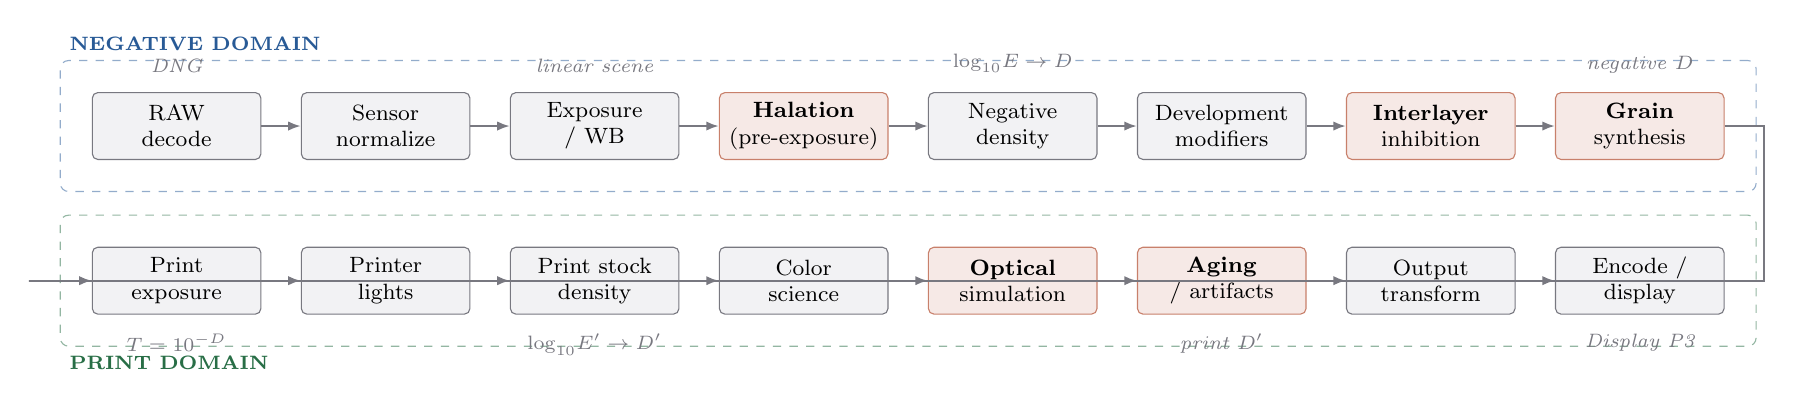
\begin{tikzpicture}[
  font=\footnotesize,
  node distance=0pt,
  stg/.style={draw=emLine, rounded corners=2pt, fill=emGray, minimum height=8.5mm,
              text width=20mm, align=center, inner sep=2pt},
  spatial/.style={stg, fill=emAcc!12, draw=emAcc!70},
  dom/.style={font=\scriptsize\itshape, text=emLine},
  ar/.style={-{Latex[length=1.6mm]}, draw=emLine, thick}
]

\node[stg] (s0) at (0,0) {RAW\\decode};
\node[stg, right=5mm of s0] (s1) {Sensor\\normalize};
\node[stg, right=5mm of s1] (s2) {Exposure\\/ WB};
\node[spatial, right=5mm of s2] (s3) {\textbf{Halation}\\(pre-exposure)};
\node[stg, right=5mm of s3] (s4) {Negative\\density};
\node[stg, right=5mm of s4] (s5) {Development\\modifiers};
\node[spatial, right=5mm of s5] (s6) {\textbf{Interlayer}\\inhibition};
\node[spatial, right=5mm of s6] (s7) {\textbf{Grain}\\synthesis};

\foreach \a/\b in {s0/s1, s1/s2, s2/s3, s3/s4, s4/s5, s5/s6, s6/s7}
  \draw[ar] (\a) -- (\b);

\node[stg, below=11mm of s0] (t0) {Print\\exposure};
\node[stg, right=5mm of t0] (t1) {Printer\\lights};
\node[stg, right=5mm of t1] (t2) {Print stock\\density};
\node[stg, right=5mm of t2] (t3) {Color\\science};
\node[spatial, right=5mm of t3] (t4) {\textbf{Optical}\\simulation};
\node[spatial, right=5mm of t4] (t5) {\textbf{Aging}\\/ artifacts};
\node[stg, right=5mm of t5] (t6) {Output\\transform};
\node[stg, right=5mm of t6] (t7) {Encode /\\display};

\foreach \a/\b in {t0/t1, t1/t2, t2/t3, t3/t4, t4/t5, t5/t6, t6/t7}
  \draw[ar] (\a) -- (\b);

\draw[ar] (s7.east) -- ++(0.5,0) |- ($(t0.west)+(-0.8,0)$) -- (t0.west);

\node[dom, above=1.2mm of s0] {DNG};
\node[dom, above=1.2mm of s2] {linear scene};
\node[dom, above=1.2mm of s4] {$\logE \to D$};
\node[dom, above=1.2mm of s7] {negative $D$};
\node[dom, below=1.2mm of t0] {$T = 10^{-D}$};
\node[dom, below=1.2mm of t2] {$\logE' \to D'$};
\node[dom, below=1.2mm of t5] {print $D'$};
\node[dom, below=1.2mm of t7] {Display P3};

\begin{scope}[on background layer]
  \node[fit=(s0)(s7), draw=emBlue!50, dashed, rounded corners=3pt, inner sep=4mm] (negbox) {};
  \node[fit=(t0)(t7), draw=emGreen!50, dashed, rounded corners=3pt, inner sep=4mm] (prbox) {};
\end{scope}
\node[above right=0mm and 0mm of negbox.north west, font=\scriptsize\bfseries, text=emBlue] {NEGATIVE DOMAIN};
\node[below right=0mm and 0mm of prbox.south west, font=\scriptsize\bfseries, text=emGreen] {PRINT DOMAIN};

\end{tikzpicture}}
\caption{The \EM{} development pipeline. Shaded stages are spatial (neighborhood-dependent) or stochastic and cannot be expressed as a lookup table. The pipeline crosses from the negative domain to the print domain by converting density to transmittance, which is the operation a physical enlarger performs.}
\label{fig:pipeline}
\end{figure*}

\subsection{Derivation of Stage Ordering}

The ordering in Figure~\ref{fig:pipeline} is not a preference. Each adjacency
is forced by physics, and the following are the binding constraints:

\begin{enumerate}
\item \textbf{Halation precedes density formation.} Scattered light is light.
It adds to the exposure that forms the latent image, so it must be summed in
the linear exposure domain \emph{before} the characteristic curve is applied.
Applying a glow after tone mapping --- the near-universal shortcut --- produces
halos whose intensity does not correctly saturate, because the shoulder has
already compressed the highlight that should have driven them. This is the
single most visible correctness difference between \EM{} and a filter.
\item \textbf{Interlayer inhibition acts on development, not on the printed
image.} Inhibitors are released during development in proportion to local
development activity, and diffuse before they can suppress neighbors.
Therefore the operator reads the developed density field and modifies it, after
the characteristic curve and before printing.
\item \textbf{Grain lives on the negative.} The dye clouds are in the negative
emulsion. Their density fluctuation is subsequently \emph{printed}, which means
the print stock's contrast amplifies negative grain --- a high-contrast print
stock makes grain more visible, exactly as in practice. Synthesizing grain
after the print transform loses this coupling and produces grain whose
visibility is independent of print contrast, which is wrong and looks wrong.
\item \textbf{Printer lights act on the print exposure, not on the negative
density.} A printer light attenuates the enlarger beam. Because the negative's
transmittance multiplies the beam, and because both are in the exposure domain,
printer lights are a multiplicative offset in linear exposure, equivalently an
additive offset in $\logE$. Section~\ref{sec:printerlights} shows why this
produces the characteristic ``rotation'' of color balance with density that a
simple RGB gain cannot.
\item \textbf{Optical simulation follows the print.} Lens artifacts belong to
the taking lens and therefore ought, strictly, to precede exposure. \EM{}
splits them: \emph{geometric and irradiance} effects (distortion, vignetting,
chromatic aberration) are applied pre-exposure where they physically belong;
\emph{appearance} effects associated with viewing and projection (bloom,
diffusion) are applied post-print. Section~\ref{sec:optical} specifies the
split and the rationale for each.
\item \textbf{Aging is last.} Physical damage to the film or print happens
after everything else and is not attenuated by any subsequent process.
\end{enumerate}

\subsection{Domain Transitions}

The pipeline traverses four distinct numerical domains, and every bug class we
anticipate arises at a transition between them. Table~\ref{tab:domains} is the
normative statement of what quantity is carried at each point.

\begin{table}[htbp]
\caption{Numerical Domains Along the Pipeline}
\label{tab:domains}
\begin{center}
\renewcommand{\arraystretch}{1.15}
\begin{tabularx}{\columnwidth}{@{}l>{\raggedright\arraybackslash}Xll@{}}
\toprule
\textbf{Domain} & \textbf{Quantity} & \textbf{Range} & \textbf{Format} \\
\midrule
Scene linear & Relative exposure $E$, $E=1$ at diffuse white & $[0, 64]$ & RGBA32F \\
Log exposure & $x = \logE$ & $[-4, +2]$ & RGBA32F \\
Negative density & $D$, Status M & $[0.1, 3.5]$ & RGBA16F \\
Print exposure & $E' = T \cdot L$ & $[0,\ 8]$ & RGBA16F \\
Print density & $D'$, Status A & $[0.05, 2.6]$ & RGBA16F \\
Display & Encoded P3 / sRGB & $[0,1]$ & RGBA8 / RGBA16F \\
\bottomrule
\end{tabularx}
\end{center}
\end{table}

Note that the format column permits \texttt{half} precision only from the
density domain onward. In density, values are compressed into roughly
$[0, 3.5]$ with meaningful resolution of $0.001$; \texttt{half} provides
approximately $0.0005$ resolution at $D=2$, which is adequate. In scene linear,
a 16-stop range requires representing $10^{-4}$ and $10^{1}$ with equal relative
precision, and \texttt{half}'s subnormal behavior near $10^{-4}$ introduces
visible shadow quantization. Constraint CR-05 exists for this reason and is
tested by NFR-06.

\subsection{Concurrency Model}

Three execution contexts exist and are strictly separated:

\begin{itemize}
\item \textbf{Main actor.} All SwiftUI state, all user input, all
\texttt{Recipe} mutation. The \texttt{Recipe} is a value type; mutations are
cheap and produce a new immutable snapshot.
\item \textbf{Render actor.} A dedicated serial \texttt{actor} owning the
\texttt{MTLCommandQueue}, the resource heap, and the pipeline state cache.
Receives immutable \texttt{Recipe} snapshots, coalesces them (only the most
recent pending snapshot is rendered --- intermediate ones are dropped), and
enqueues GPU work.
\item \textbf{I/O queue.} A concurrent \texttt{DispatchQueue} for RAW decode,
thumbnail generation, database writes, and export encoding.
\end{itemize}

The coalescing behavior on the render actor is what makes slider dragging feel
correct. During a drag, parameter updates arrive at up to 120\,Hz while the
render takes 8--16\,ms. Queueing every update produces mounting latency; the
render actor therefore holds a single \texttt{pendingRecipe} slot, overwrites
it on each update, and picks up the latest value when the previous frame's
command buffer completes. This is specified in Section~\ref{sec:apparch} with
the full state machine.

\section{Color Management and the Working Space}
\label{sec:colorspace}

\subsection{RAW Decode Configuration}
\label{sec:raw-config}

The correctness of every subsequent stage rests on obtaining a genuinely
scene-referred linear image. Apple's RAW pipeline \cite{coreimage} defaults are
tuned to produce a pleasing display-referred result, and every one of those
defaults is destructive to our purposes. The required configuration is:

\begin{lstlisting}[language=Swift, caption={Scene-referred RAW decode configuration.}, label={lst:rawconfig}]
func makeSceneReferredFilter(url: URL) throws -> CIFilter & CIRAWFilter {
    guard let f = CIRAWFilter(imageURL: url) else { throw DecodeError.unsupported }

    // 1. Defeat every rendering intent Apple applies by default.
    f.isGamutMappingEnabled       = false
    f.localToneMapAmount          = 0.0
    f.extendedDynamicRangeAmount  = 0.0   // we manage headroom ourselves
    f.boostAmount                 = 0.0   // disables the S-curve entirely
    f.boostShadowAmount           = 0.0
    f.contrastAmount              = 0.0
    f.shadowBias                  = 0.0

    // 2. Defeat spatial processing we intend to model ourselves.
    f.sharpnessAmount             = 0.0
    f.detailAmount                = 0.0
    f.contrastAmount              = 0.0
    f.luminanceNoiseReductionAmount = 0.0
    f.colorNoiseReductionAmount     = 0.0

    // 3. Keep the vendor's geometric and shading corrections: these are
    //    calibration, not interpretation, and reimplementing them is
    //    value-destructive.
    f.isLensCorrectionEnabled     = true

    // 4. Preserve capture white balance as the *starting point*; the user
    //    may override, but we must know what the camera decided.
    f.neutralTemperature          = f.neutralTemperature
    f.neutralTint                 = f.neutralTint

    return f
}
\end{lstlisting}

The decoded image is requested in a linear working color space with an
extended range, and the render destination is configured with
\texttt{CIContext} options that disable any output color management, because
the render graph performs its own conversion:

\begin{lstlisting}[language=Swift, caption={Context configuration for linear extended-range output.}]
let ws = CGColorSpace(name: CGColorSpace.extendedLinearDisplayP3)!
let ctx = CIContext(mtlDevice: device, options: [
    .workingColorSpace  : ws,
    .workingFormat      : CIFormat.RGBAf,
    .cacheIntermediates : false,
    .highQualityDownsample : true
])
\end{lstlisting}

\subsection{Choice of Working Space}

The pipeline requires a working space that (i) encloses the gamut of every
iPhone sensor after color matrix application, (ii) encloses the gamut of the
modelled film dyes, which extend outside Rec.\,709 in the cyan and yellow
regions, (iii) has a white point compatible with the printing model, and (iv)
has a documented, invertible relationship to CIE XYZ \cite{hunt2011}.

Three candidates were evaluated:

\begin{table}[htbp]
\caption{Working Space Evaluation}
\label{tab:workingspace}
\begin{center}
\renewcommand{\arraystretch}{1.15}
\begin{tabularx}{\columnwidth}{@{}l>{\raggedright\arraybackslash}X@{}}
\toprule
\textbf{Space} & \textbf{Assessment} \\
\midrule
Linear Display P3 & Native to the platform, zero-cost preview conversion, but clips saturated cyans that the modelled cyan dye reaches. Rejected as primary; retained as the display target. \\
ACEScg (AP1) & Wide enough, industry standard, well-documented transforms, D60 white point requires adaptation to D65 for display. Chosen. \\
DaVinci Wide Gamut & Wider still, excellent for interchange with Resolve, but the transform is vendor-published rather than standardized. Retained as an export option only. \\
\bottomrule
\end{tabularx}
\end{center}
\end{table}

\EM{} adopts \textbf{ACEScg} \cite{acescg,st2065} (ACES AP1 primaries, linear,
D60 white) as the
internal scene-referred working space. The choice costs one matrix multiply on
input and one on output relative to staying in Display P3, and buys gamut
headroom that prevents negative-valued channels from appearing mid-pipeline ---
which matters enormously, because $\logE$ of a negative number is undefined and
a single clamped channel produces a visible hue shift in saturated highlights.

\subsection{Input Transform}

The decoded image arrives in extended linear Display P3. The conversion to
ACEScg is the composition of the P3-to-XYZ matrix, a Bradford
\cite{lam1985} chromatic
adaptation from D65 to D60, and the XYZ-to-AP1 matrix:

\begin{equation}
\mathbf{M}_{\mathrm{in}} = \mathbf{M}_{\mathrm{XYZ}\to\mathrm{AP1}}\,
\mathbf{M}_{\mathrm{CAT}}^{\mathrm{D65}\to\mathrm{D60}}\,
\mathbf{M}_{\mathrm{P3}\to\mathrm{XYZ}}
\label{eq:min}
\end{equation}

evaluating numerically to

\begin{equation}
\mathbf{M}_{\mathrm{in}} \approx
\begin{pmatrix}
\phantom{-}0.9525 & \phantom{-}0.0343 & \phantom{-}0.0132 \\
\phantom{-}0.0170 & \phantom{-}0.9754 & \phantom{-}0.0076 \\
-0.0018 & \phantom{-}0.0107 & \phantom{-}0.9911
\end{pmatrix}.
\label{eq:minval}
\end{equation}

The matrix is precomputed on the host at profile-load time, not in the shader.

The inverse transform for the display path is $\mathbf{M}_{\mathrm{out}} =
\mathbf{M}_{\mathrm{in}}^{-1}$ followed by the Display P3 transfer function.

\subsection{Exposure Normalization and the Anchor Problem}

Film responds to absolute exposure; a digital sensor reports a relative value
scaled by an unknown gain. Before the characteristic curve can be applied, the
image must be anchored so that a known scene reflectance maps to a known
position on the curve.

\EM{} adopts the standard cinematographic anchor: an 18\% diffuse reflector
under correct exposure maps to a relative exposure of $E = 0.18$ in the working
space, which is placed at the film's rated speed point. The transformation is

\begin{equation}
E_{\mathrm{anchored}} = E_{\mathrm{decoded}} \cdot 2^{\,\varepsilon} \cdot
\frac{0.18}{g_{\mathrm{cal}}}
\label{eq:anchor}
\end{equation}

where $\varepsilon$ is the user's exposure compensation in stops and
$g_{\mathrm{cal}}$ is a per-device calibration constant relating the decoded
middle-gray value to the working-space unit. Determining $g_{\mathrm{cal}}$ is a
calibration task, specified in Section~\ref{sec:calibration}; a wrong
$g_{\mathrm{cal}}$ manifests as every image sitting too high or too low on the
characteristic curve, which the user experiences as ``the stocks all look
flat'' or ``everything blocks up.''

The relation between anchored exposure and the film's rated ISO speed $S$ is

\begin{equation}
\logE_{\mathrm{film}} = \log_{10}\!\left(E_{\mathrm{anchored}}\right)
+ \log_{10}\!\left(\frac{S}{S_0}\right) + x_{\mathrm{ref}}
\label{eq:isoshift}
\end{equation}

with $S_0 = 100$ the reference speed and $x_{\mathrm{ref}}$ the stock's
speed-point log exposure. This is what makes ``shooting Portra 400 at 800''
meaningful: it shifts $\logE_{\mathrm{film}}$ by $-0.301$, moving the entire
image down the characteristic curve into the toe, which the user then
compensates for by pushing development (Section~\ref{sec:development}) ---
exactly the real relationship, produced by the model rather than scripted.

\subsection{White Balance in the Working Space}

White balance is applied as a von Kries adaptation in the LMS cone space rather
than as an RGB channel gain, because channel gain in a wide-gamut space
produces hue rotation in saturated colors. The operator is

\begin{equation}
\mathbf{E}' = \mathbf{M}_{\mathrm{AP1}\to\mathrm{LMS}}^{-1}\,
\mathrm{diag}\!\left(\frac{\boldsymbol{\rho}_{\mathrm{dst}}}{\boldsymbol{\rho}_{\mathrm{src}}}\right)
\mathbf{M}_{\mathrm{AP1}\to\mathrm{LMS}}\, \mathbf{E}
\label{eq:vonkries}
\end{equation}

where $\boldsymbol{\rho}$ are the cone responses to the source and destination
illuminants and $\mathbf{M}_{\mathrm{AP1}\to\mathrm{LMS}}$ uses the CAT02
\cite{cie159}
transform. Because both matrices and the diagonal are constant per frame, the
whole of \eqref{eq:vonkries} collapses to a single $3\times3$ matrix computed on
the host, so the shader cost is one matrix multiply.

\subsection{Tungsten Stocks and the Illuminant Question}

A tungsten-balanced stock such as Vision3 500T is not a color filter. It is an
emulsion whose three layers have different relative sensitivities, calibrated so
that a 3200\,K illuminant produces equal densities. Modelling it as a blue push
is wrong; the correct model is a per-layer speed offset $\Delta x_c$ applied to
the log exposure before the characteristic curve:

\begin{equation}
x_c \leftarrow x_c + \Delta x_c^{\mathrm{(balance)}}, \quad c \in \{R,G,B\}
\label{eq:tungsten}
\end{equation}

with $\Delta x^{\mathrm{(balance)}}$ derived from the ratio of the stock's
layer sensitivities integrated against the reference illuminant SPD. For a
tungsten stock shot under daylight without correction, this produces the
familiar strong blue cast --- and, importantly, produces it \emph{with the
correct nonlinearity}, because the blue record is driven far up its curve while
red sits low, so the cast varies with scene luminance rather than being a
uniform tint. Table~\ref{tab:balance} gives the shipping values.

\begin{table}[htbp]
\caption{Layer Balance Offsets $\Delta x^{\mathrm{(balance)}}$}
\label{tab:balance}
\begin{center}
\renewcommand{\arraystretch}{1.15}
\begin{tabular}{@{}lccc@{}}
\toprule
\textbf{Stock class} & $\Delta x_R$ & $\Delta x_G$ & $\Delta x_B$ \\
\midrule
Daylight (5500\,K aim)  & $0.000$ & $0.000$ & $0.000$ \\
Tungsten (3200\,K aim)  & $-0.310$ & $-0.055$ & $+0.365$ \\
Type L long-exposure    & $-0.285$ & $-0.040$ & $+0.325$ \\
Monochrome panchromatic & $0.000$ & $0.000$ & $0.000$ \\
\bottomrule
\end{tabular}
\end{center}
\end{table}

\section{The Digital Negative: Characteristic Curve Model}
\label{sec:negative}

\subsection{Requirements on the Curve Model}

The transfer from log exposure to optical density is the mathematical heart of
the application. The model must satisfy six requirements:

\begin{enumerate}
\item \textbf{R1.} Reproduce the toe, straight-line, and shoulder regions of a
measured $D$--$\logE$ curve to within AC-1 tolerance.
\item \textbf{R2.} Provide \emph{independent} control of each region. A change
to shoulder sharpness must not move the speed point; a change to gamma must not
change $\Dmax$.
\item \textbf{R3.} Be $C^\infty$. Any discontinuity in the first derivative
produces a visible contour in a smooth gradient, and any discontinuity in the
second derivative is visible in a sky.
\item \textbf{R4.} Have a closed-form derivative, because the derivative
\emph{is} the local gamma, which the grain model
(Section~\ref{sec:grain}) requires pointwise.
\item \textbf{R5.} Be monotonically non-decreasing for all reachable
parameters (AC-6).
\item \textbf{R6.} Evaluate in a handful of GPU instructions.
\end{enumerate}

Spline-fit tables satisfy R1 and R6 but violate R2 catastrophically --- moving
one control point changes the curve globally in ways that do not correspond to
any physical parameter, which destroys parameter honesty. The classical
Hurter--Driffield treatment \cite{hurter1890,james1977} gives the straight line
but no closed form for the extremes. Generalized logistic (Richards) curves are $C^\infty$ and monotone but
couple toe and shoulder sharpness through a single asymmetry exponent, failing
R2.

\subsection{The Softplus Density Model}

\EM{} uses a formulation built from softplus primitives. Define the softplus
with sharpness parameter $a > 0$:

\begin{equation}
\softp{a}{u} \;=\; a \ln\!\left(1 + e^{u/a}\right).
\label{eq:softplus}
\end{equation}

This function is the canonical smooth relaxation of $\max(u, 0)$: it is
$C^\infty$, strictly increasing, satisfies $\softp{a}{u} \to \max(u,0)$ as $a
\to 0^+$, and has the logistic function as its derivative,
$\tfrac{d}{du}\softp{a}{u} = \sigma(u/a)$ with $\sigma(t) = (1+e^{-t})^{-1}$.

Let $x = \logE$ be the log exposure reaching a given layer, and define the
straight-line coordinate

\begin{equation}
u(x) \;=\; \gamma\,\big(x - x_{0}\big),
\label{eq:ucoord}
\end{equation}

where $\gamma$ is the straight-line gamma and $x_0$ is the \emph{extrapolated
speed point}: the log exposure at which the straight-line portion, extended
downward, intersects $\Dmin$.

The characteristic curve is then

\begin{equation}
\boxed{\;D(x) \;=\; \Dmin \;+\; \softp{\kappa_t}{u(x)} \;-\; \softp{\kappa_s}{u(x) - \Delta D}\;}
\label{eq:charcurve}
\end{equation}

with $\Delta D = \Dmax - \Dmin$ the density range, $\kappa_t > 0$ the toe
softness, and $\kappa_s > 0$ the shoulder softness.

\subsection{Behavior and Verification of the Model}

The three asymptotic regimes follow directly from \eqref{eq:softplus}:

\paragraph{Toe, $u \ll 0$} Both softplus terms vanish exponentially and $D \to
\Dmin$. Approach is exponential with scale $\kappa_t/\gamma$ in log exposure,
matching the observed sub-threshold behavior of real emulsions.

\paragraph{Straight line, $\kappa_t \ll u \ll \Delta D - \kappa_s$} The first
term is $\approx u$, the second $\approx 0$, giving

\begin{equation}
D(x) \approx \Dmin + \gamma\,(x - x_0),
\end{equation}

a line of slope exactly $\gamma$ intercepting $\Dmin$ at $x_0$, as required by
R2.

\paragraph{Shoulder, $u \gg \Delta D$} The first term is $\approx u$, the
second $\approx u - \Delta D$, and $D \to \Dmin + \Delta D = \Dmax$.

\medskip
The derivative --- the \emph{point gamma} $\gamma(x)$ --- is available in closed
form, satisfying R4:

\begin{equation}
\boxed{\;\gamma(x) \;=\; \frac{dD}{dx} \;=\; \gamma\left[\sigma\!\left(\frac{u}{\kappa_t}\right) - \sigma\!\left(\frac{u - \Delta D}{\kappa_s}\right)\right]\;}
\label{eq:pointgamma}
\end{equation}

Monotonicity (R5) follows immediately: $\sigma$ is strictly increasing, and
since $u > u - \Delta D$ whenever $\Delta D > 0$, we have $\sigma(u/\kappa_t) >
\sigma((u-\Delta D)/\kappa_s)$ provided $\kappa_t \le \kappa_s$ or, more
generally, provided $\Delta D$ is large relative to the softness parameters.
The precise condition is stated below.

\subsection{Well-Formedness Condition}

The two softplus terms overlap when $\Delta D$ is not large compared to
$\kappa_t + \kappa_s$, in which case the curve never reaches $\Dmax$ and, in the
extreme, can become non-monotone. Evaluating \eqref{eq:pointgamma} at the
midpoint $u = \Delta D/2$ gives the minimum-margin case; requiring
$\gamma(x) > 0$ everywhere yields the sufficient condition

\begin{equation}
\Delta D \;>\; \left(\kappa_t + \kappa_s\right)\ln\!\left(\frac{\kappa_s}{\kappa_t}\right)
\quad\text{when } \kappa_s > \kappa_t,
\label{eq:wellformed1}
\end{equation}

and monotonicity is unconditional when $\kappa_s \le \kappa_t$. In practice
\EM{} enforces the stricter engineering constraint

\begin{equation}
\Delta D \;\geq\; 4\left(\kappa_t + \kappa_s\right),
\label{eq:wellformed}
\end{equation}

which additionally guarantees that the attained maximum density is within
$0.02$ density units of the nominal $\Dmax$ and that a genuine straight-line
region of at least $\Delta D / 2$ exists. The parameter validator in
\texttt{EmulsionCore} rejects any profile violating \eqref{eq:wellformed} at
load time, and the UI clamps $\kappa$ sliders so that the condition cannot be
violated interactively.

\subsection{Per-Record Parameterization and the Orange Mask}

Each color record has an independent parameter set
$\theta_c = (\Dmin{}_{,c}, \Delta D_c, \gamma_c, x_{0,c}, \kappa_{t,c},
\kappa_{s,c})$, $c \in \{R,G,B\}$, so \eqref{eq:charcurve} is evaluated three
times.

The $\Dmin$ vector deserves specific attention because it encodes the
\emph{orange mask} of color negative film. Colored couplers in the magenta and
cyan layers absorb blue and green light even where undeveloped, producing the
familiar orange base. In Status M density \cite{iso5} this appears as

\begin{equation}
\Dmin^{\mathrm{(colorneg)}} \approx (0.58,\; 0.92,\; 1.28)^\top
\end{equation}

for a typical modern stock. The mask is not decorative: it is an
inter-image correction that compensates for unwanted absorptions of the cyan
and magenta dyes, and it is calibrated to be removed by the printing stage.
Modelling the mask but failing to model its removal produces the ``scanned
negative that was never printed'' look --- muddy, low-saturation, warm ---
which is a real and recognizable failure mode. Section~\ref{sec:print}
specifies the removal.

Because the mask density is largely independent of exposure, it can be carried
as a constant offset. \EM{} nevertheless models a small exposure dependence,
since real masking couplers are consumed in proportion to development:

\begin{equation}
\Dmin{}_{,c}(x) = \Dmin{}_{,c}^{(0)} - m_c \cdot \frac{D_c(x) - \Dmin{}_{,c}^{(0)}}{\Delta D_c},
\label{eq:maskdepletion}
\end{equation}

with $m_c$ the mask depletion coefficient, typically $(0.00, 0.06, 0.10)$.
Equation \eqref{eq:maskdepletion} is applied as a single fixed-point iteration
rather than solved exactly; the correction is small and one iteration is
below the AC-1 tolerance.

\subsection{Curve Family Illustration}

Figure~\ref{fig:charcurve} plots \eqref{eq:charcurve} for the three records of a
representative daylight color negative stock, and
Figure~\ref{fig:pointgamma} plots the corresponding point gamma
\eqref{eq:pointgamma}.

\begin{figure}[htbp]
\centering
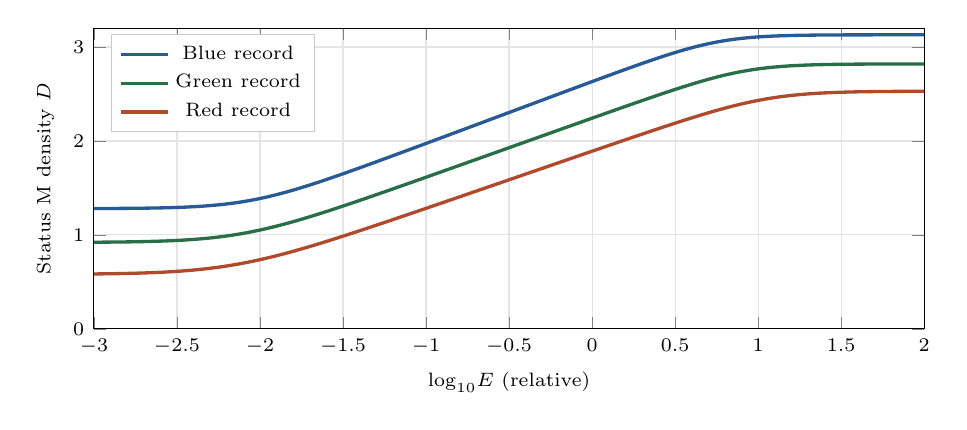
\begin{tikzpicture}
\begin{axis}[
  width=\columnwidth, height=5.4cm,
  xlabel={$\logE$ (relative)},
  ylabel={Status M density $D$},
  xmin=-3, xmax=2, ymin=0, ymax=3.2,
  grid=both, grid style={draw=emLine!20},
  legend style={font=\scriptsize, at={(0.02,0.98)}, anchor=north west, draw=emLine!40},
  label style={font=\scriptsize}, tick label style={font=\scriptsize},
  samples=250,
]
% Blue record (highest Dmin, mask)
\addplot[emBlue, very thick, domain=-3:2]
  {1.28 + 0.13*ln(1+exp((0.66*(x+2.05))/0.13)) - 0.11*ln(1+exp((0.66*(x+2.05)-1.85)/0.11))};
\addlegendentry{Blue record}
% Green record
\addplot[emGreen, very thick, domain=-3:2]
  {0.92 + 0.14*ln(1+exp((0.63*(x+2.10))/0.14)) - 0.11*ln(1+exp((0.63*(x+2.10)-1.90)/0.11))};
\addlegendentry{Green record}
% Red record
\addplot[emAcc, very thick, domain=-3:2]
  {0.58 + 0.15*ln(1+exp((0.61*(x+2.15))/0.15)) - 0.12*ln(1+exp((0.61*(x+2.15)-1.95)/0.12))};
\addlegendentry{Red record}
\end{axis}
\end{tikzpicture}
\caption{Characteristic curves from \eqref{eq:charcurve} for a daylight color negative stock. The vertical separation at the base is the orange mask. Note that the three records are near-parallel through the straight-line region --- non-parallelism is \emph{crossover}, and it is the dominant cause of colors that cannot be corrected by a global balance change.}
\label{fig:charcurve}
\end{figure}

\begin{figure}[htbp]
\centering
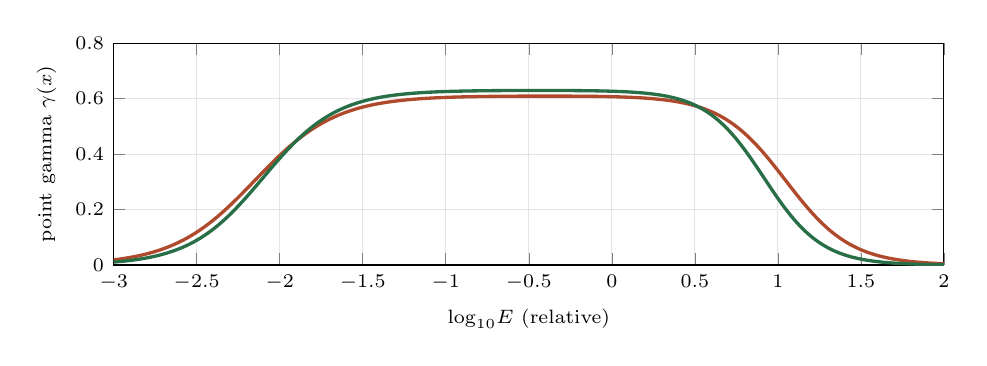
\begin{tikzpicture}
\begin{axis}[
  width=\columnwidth, height=4.4cm,
  xlabel={$\logE$ (relative)},
  ylabel={point gamma $\gamma(x)$},
  xmin=-3, xmax=2, ymin=0, ymax=0.8,
  grid=both, grid style={draw=emLine!20},
  label style={font=\scriptsize}, tick label style={font=\scriptsize},
  samples=250,
]
\addplot[emAcc, very thick, domain=-3:2]
  {0.61*( 1/(1+exp(-(0.61*(x+2.15))/0.15)) - 1/(1+exp(-(0.61*(x+2.15)-1.95)/0.12)) )};
\addplot[emGreen, very thick, domain=-3:2]
  {0.63*( 1/(1+exp(-(0.63*(x+2.10))/0.14)) - 1/(1+exp(-(0.63*(x+2.10)-1.90)/0.11)) )};
\end{axis}
\end{tikzpicture}
\caption{Point gamma from \eqref{eq:pointgamma} for the red and green records. The plateau is the straight line; the rise and fall are the toe and shoulder. This function is consumed directly by the grain variance model \eqref{eq:grainvar} and by the interlayer inhibition weighting.}
\label{fig:pointgamma}
\end{figure}

\subsection{Derived Sensitometric Quantities}

The following quantities are computed from $\theta_c$ on the host and exposed
in the UI as read-only diagnostics. They are the standard vocabulary of
sensitometry and their presence is a substantial part of the product's claim to
professional seriousness.

\paragraph{Speed point} The log exposure producing density $\Dmin + 0.10$:

\begin{equation}
x_{\mathrm{sp}} = x_0 + \frac{\kappa_t}{\gamma}\ln\!\left(e^{0.10/\kappa_t} - 1\right).
\label{eq:speedpoint}
\end{equation}

This inverts the toe branch of \eqref{eq:charcurve} exactly, since the shoulder
term is negligible at this density. ISO speed follows as $S = 0.8 /
10^{x_{\mathrm{sp}}}$ in the arithmetic scale \cite{iso5800,iso6}.

\paragraph{Contrast index} Following standard sensitometric practice
\cite{kodakh740}, the slope of the chord
from the speed point to a point $2.00$ log-exposure units higher:

\begin{equation}
\mathrm{CI} = \frac{D(x_{\mathrm{sp}} + 2.00) - D(x_{\mathrm{sp}})}{2.00}.
\label{eq:ci}
\end{equation}

For a normal-process color negative $\mathrm{CI} \approx 0.55$--$0.62$; for
black-and-white pictorial negatives $0.50$--$0.58$.

\paragraph{Useful exposure latitude} The interval over which point gamma
exceeds a fraction $\lambda$ of its maximum (default $\lambda = 0.5$),
obtained by solving $\gamma(x) = \lambda\gamma_{\max}$ numerically with two
Newton steps from the analytic straight-line bracket. Reported in stops as
$\mathrm{L} = (x_{\mathrm{hi}} - x_{\mathrm{lo}})/\log_{10} 2$. Modern color
negative stocks report 12--14 stops by this measure, which is why the format
tolerates overexposure so gracefully --- and why the model, if correct,
reproduces that tolerance without a special case.

\subsection{Monochrome Stocks}

Monochrome emulsions use the same formulation with a single parameter set and a
spectral weighting applied before \eqref{eq:charcurve} to convert the
three-channel working image into the single exposure the panchromatic layer
receives:

\begin{equation}
E_{\mathrm{pan}} = \mathbf{w}^\top \mathbf{E}, \qquad
\mathbf{w} = \mathbf{w}_{\mathrm{spectral}} \odot \mathbf{w}_{\mathrm{filter}},
\label{eq:pan}
\end{equation}

where $\mathbf{w}_{\mathrm{spectral}}$ is the stock's normalized spectral
sensitivity integrated against the AP1 primaries and
$\mathbf{w}_{\mathrm{filter}}$ models an optional contrast filter (yellow,
orange, red, green) \cite{kodakh1}. This is the mechanism by which a red filter darkens a blue
sky in \EM{} for the same reason it does on a real camera, rather than by a
scripted sky-darkening effect. Default weights for a panchromatic stock are
$\mathbf{w}_{\mathrm{spectral}} = (0.30, 0.59, 0.11)$; an orthochromatic
profile uses $(0.02, 0.68, 0.30)$, which correctly renders red lips dark.

\subsection{Shader Implementation}

Equation~\eqref{eq:charcurve} costs two \texttt{log}, two \texttt{exp}, and
approximately ten fused multiply-adds per channel. The naive evaluation
overflows for large $u/\kappa$; the numerically stable form used in the shader
is

\begin{equation}
\softp{a}{u} = \max(u, 0) + a\ln\!\left(1 + e^{-|u|/a}\right),
\label{eq:softplus-stable}
\end{equation}

which is exact and never evaluates $e^{t}$ for $t > 0$.

\begin{lstlisting}[language=Metal, caption={Stable characteristic curve evaluation.}, label={lst:charcurve}]
inline float softplus_stable(float u, float a) {
    // sp_a(u) = max(u,0) + a*log1p(exp(-|u|/a))
    return max(u, 0.0f) + a * log1p(exp(-abs(u) / a));
}

inline float3 characteristic_curve(float3 logE, constant StockParams &p) {
    float3 u = p.gamma * (logE - p.x0);
    float3 sp_t, sp_s;
    for (uint c = 0; c < 3; ++c) {
        sp_t[c] = softplus_stable(u[c],              p.kappa_t[c]);
        sp_s[c] = softplus_stable(u[c] - p.dD[c],    p.kappa_s[c]);
    }
    return p.dMin + sp_t - sp_s;
}

inline float3 point_gamma(float3 logE, constant StockParams &p) {
    float3 u = p.gamma * (logE - p.x0);
    float3 a = 1.0f / (1.0f + exp(-u / p.kappa_t));
    float3 b = 1.0f / (1.0f + exp(-(u - p.dD) / p.kappa_s));
    return p.gamma * (a - b);
}
\end{lstlisting}

Note that \texttt{log1p} is required rather than \texttt{log(1+x)}: for large
$|u|/a$ the argument $e^{-|u|/a}$ underflows toward zero and $\log(1+x)$ loses
all significant digits, producing a stair-stepped toe that is plainly visible in
deep shadow. This is the kind of defect that survives casual review and is
caught only by the ramp test in NFR-06.

\section{Chemical Development Modelling}
\label{sec:development}

\subsection{What Development Actually Changes}

Development converts the latent image into density. Varying the development
process does not translate the characteristic curve; it \emph{reshapes} it, and
the reshaping is highly structured:

\begin{itemize}
\item \textbf{Gamma rises with development, then saturates.} More development
time develops more of the exposed crystals, steepening the curve --- but only
until essentially all exposed crystals are developed, after which further time
produces only fog. The classical gamma-versus-time family
\cite{james1977,kodakh740} is asymptotic to a
value $\gamma_\infty$ characteristic of the emulsion and developer.
\item \textbf{Fog rises without bound.} Unexposed crystals develop
spontaneously at a slow rate, raising $\Dmin$ indefinitely. This is why heavy
pushing produces flat, milky shadows: the shadow density is fog, and fog
carries no image.
\item \textbf{Speed gain is much smaller than the exposure deficit.} A
two-stop push does not recover two stops. It recovers, typically, one third to
one half of a stop of true speed, because the toe crystals that received too
few photons never formed a developable latent image and no amount of
development creates one. The rest of the apparent gain is contrast increase.
\end{itemize}

The last point is the one that consumer applications universally miss, and it
is the reason \EM{}'s push processing looks correct: pushed images have
\emph{empty, contrasty shadows}, not brighter shadows.

\subsection{Development Activity}

All process variables --- time, temperature, agitation, developer strength ---
are collapsed into a single scalar \emph{development activity} $A$, normalized
so that $A = 1$ is the manufacturer's normal process. Time and temperature
combine through an Arrhenius relation on the reaction rate:

\begin{equation}
A \;=\; \frac{t}{t_0}\,\exp\!\left[\frac{E_a}{R}\left(\frac{1}{T_0} - \frac{1}{T}\right)\right]\, \eta(a_g)\, \frac{[\mathrm{dev}]}{[\mathrm{dev}]_0},
\label{eq:activity}
\end{equation}

where $t$ is development time, $T$ is absolute temperature in kelvin, $E_a$ is
the apparent activation energy of the development reaction, $R$ is the gas
constant, $\eta(a_g)$ is an agitation efficiency factor, and the final factor
is relative developer concentration. For standard color negative chemistry
$E_a/R \approx 8.4 \times 10^3$\,K, which yields the familiar rule of thumb that
a $\pm 0.5$\textdegree C error at 38\textdegree C is roughly a $\pm 4.5\%$ change
in effective time. Reproducing that sensitivity is what makes the temperature
control feel like a real process control rather than a slider.

Agitation efficiency uses a saturating form,

\begin{equation}
\eta(a_g) = \eta_\infty - (\eta_\infty - \eta_0)\,e^{-a_g/a_c},
\end{equation}

normalized so that $\eta(1) = 1$ at the recommended agitation scheme. Reduced
agitation ($a_g < 1$) both lowers activity and, importantly, \emph{increases}
the interlayer adjacency effect of Section~\ref{sec:interlayer}, because
exhausted developer and released inhibitor are not swept away from the emulsion
surface. This coupling is modelled explicitly and is the mechanism behind
stand-development's characteristic edge effects.

\subsection{Parameter Modulation}

Given $A$ and a push/pull setting of $n$ stops (positive is push), the stock's
nominal parameters $\theta^{(0)}$ are modulated as follows. Push and pull are
expressed through $A$ --- a push of $n$ stops corresponds to
$A = A_0 \cdot \rho^{\,n}$ with $\rho \approx 1.35$ per stop for color negative
chemistry --- so there is a single mechanism, not two.

\paragraph{Gamma} follows the saturating development curve:

\begin{equation}
\gamma(A) \;=\; \gamma_\infty\left(1 - e^{-A/A_\gamma}\right),
\label{eq:gammatime}
\end{equation}

with $A_\gamma$ chosen per stock so that $\gamma(1) = \gamma^{(0)}$, i.e.

\begin{equation}
A_\gamma = \left[\ln\!\left(\frac{\gamma_\infty}{\gamma_\infty - \gamma^{(0)}}\right)\right]^{-1}.
\end{equation}

Typical values are $\gamma_\infty \approx 1.6\,\gamma^{(0)}$, so that gamma can
rise substantially but not without limit. This single equation is why extreme
pushes stop adding contrast --- the correct behavior, obtained for free.

\paragraph{Fog} rises monotonically and without saturation:

\begin{equation}
\Dmin(A) \;=\; \Dmin^{(0)} + \phi_0\left(A^{\,\beta_f} - 1\right),
\label{eq:fog}
\end{equation}

with $\beta_f \approx 2.1$ and $\phi_0 \approx 0.045$ for color negative
stocks. The per-channel $\phi_0$ is not equal --- the blue-sensitive layer fogs
fastest --- which produces the characteristic cool-shadow crossover of
heavily pushed color film.

\paragraph{Speed} shifts by a fraction of the nominal push:

\begin{equation}
x_0(A) \;=\; x_0^{(0)} \;-\; \alpha_s \log_{10} A,
\label{eq:speedshift}
\end{equation}

with the \emph{speed recovery coefficient} $\alpha_s \in [0.25, 0.45]$,
substantially less than the $1.0$ that would represent full speed recovery.
Table~\ref{tab:pushresp} gives the resulting behavior, which matches published
push-processing data closely.

\paragraph{Toe softness} increases with development, because heavy development
extends the toe region as marginally-exposed crystals begin to develop:

\begin{equation}
\kappa_t(A) = \kappa_t^{(0)}\left(1 + \tau_t \ln A\right), \quad \tau_t \approx 0.30.
\end{equation}

\paragraph{Density range} rises modestly, since the shoulder is set primarily
by silver and coupler availability rather than by development:

\begin{equation}
\Delta D(A) = \Delta D^{(0)}\left(1 + \tau_D \ln A\right), \quad \tau_D \approx 0.12.
\end{equation}

\begin{table}[htbp]
\caption{Modelled Push/Pull Response, Typical Color Negative}
\label{tab:pushresp}
\begin{center}
\renewcommand{\arraystretch}{1.15}
\begin{tabular}{@{}lccccc@{}}
\toprule
\textbf{Setting} & $A$ & $\gamma$ & $\Delta\Dmin$ & \textbf{True} & \textbf{CI} \\
 & & & & \textbf{speed} & \\
\midrule
Pull 2  & $0.55$ & $0.44$ & $-0.02$ & $-0.24$\,EV & $0.41$ \\
Pull 1  & $0.74$ & $0.53$ & $-0.01$ & $-0.13$\,EV & $0.49$ \\
Normal  & $1.00$ & $0.61$ & $\phantom{-}0.00$ & $\phantom{-}0.00$\,EV & $0.58$ \\
Push 1  & $1.35$ & $0.69$ & $+0.05$ & $+0.15$\,EV & $0.66$ \\
Push 2  & $1.82$ & $0.77$ & $+0.13$ & $+0.29$\,EV & $0.73$ \\
Push 3  & $2.46$ & $0.83$ & $+0.28$ & $+0.42$\,EV & $0.79$ \\
\bottomrule
\multicolumn{6}{@{}p{0.95\columnwidth}@{}}{\footnotesize A three-stop push yields $0.42$\,EV of genuine speed. The remaining apparent gain is contrast, and the cost is $+0.28$ of fog in the shadows.}
\end{tabular}
\end{center}
\end{table}

\subsection{Cross-Processing}

Cross-processing --- developing color negative film in reversal chemistry
(C-41 in E-6) or the reverse --- is modelled as a substitution of the entire
modulation parameter set rather than as an extra effect. The mechanism is a
\emph{chemistry profile} that supplies $(\gamma_\infty, \phi_0, \beta_f,
\alpha_s, \tau_t, \tau_D)$ and a per-channel activity scaling
$\mathbf{A}_{\mathrm{chem}}$. Because the layers of a stock designed for one
chemistry respond with wildly different efficiency to another, the per-channel
activity scaling is far from unity --- for E-6 chemistry applied to a C-41
stock, approximately $(1.8, 1.1, 0.6)$ --- which is precisely what produces
cross-processing's extreme contrast and violent color crossover. Again, the
effect emerges from the model rather than being authored.

\begin{table}[htbp]
\caption{Chemistry Profiles}
\label{tab:chemistry}
\begin{center}
\renewcommand{\arraystretch}{1.15}
\begin{tabular}{@{}lccccc@{}}
\toprule
\textbf{Process} & $\gamma_\infty/\gamma^{(0)}$ & $\phi_0$ & $\beta_f$ & $\alpha_s$ & $\rho$ \\
\midrule
C-41 (color neg.)   & $1.60$ & $0.045$ & $2.1$ & $0.35$ & $1.35$ \\
E-6 (reversal)      & $1.35$ & $0.020$ & $1.7$ & $0.28$ & $1.30$ \\
ECN-2 (motion pic.) & $1.55$ & $0.030$ & $2.0$ & $0.33$ & $1.32$ \\
B\&W, general       & $2.10$ & $0.035$ & $2.4$ & $0.42$ & $1.45$ \\
B\&W, compensating  & $1.45$ & $0.025$ & $1.9$ & $0.38$ & $1.25$ \\
\bottomrule
\end{tabular}
\end{center}
\end{table}

\subsection{Where This Executes}

All of Section~\ref{sec:development} is host-side arithmetic. The development
model consumes the stock profile and the user's process parameters and produces
a modified $\theta$, which is uploaded as a small constant buffer. Nothing in
this section costs a GPU instruction, which is worth stating explicitly:
substantial perceived sophistication in the product is free at render time
because it modulates parameters rather than pixels.

This has an important corollary for the UI. Development controls can update at
unlimited rate without any incremental render cost beyond one re-render, and
they invalidate the baked pointwise LUT (Section~\ref{sec:lutbake}) but nothing
spatial. The dependency tracking in Section~\ref{sec:rendergraph} encodes this.

\section{Interlayer Inhibition and Adjacency Effects}
\label{sec:interlayer}

\subsection{The Mechanism}

Modern color negative films incorporate Development Inhibitor Releasing (DIR)
couplers \cite{james1977}. When development proceeds at a point in a layer, these couplers
release a soluble inhibitor that diffuses laterally within the layer and
vertically into adjacent layers, locally suppressing further development.

Two distinct and separately visible consequences follow:

\begin{enumerate}
\item \textbf{Intra-layer adjacency (acutance).} A densely developed region
suppresses development just outside its boundary, producing a light rim on the
low-density side of an edge --- the Eberhard effect. Because the suppression is
proportional to neighborhood density and subtracted locally, the net operator is
an unsharp mask applied in the density domain. This is why color negative film
has apparent sharpness exceeding what its MTF alone would predict, and why it
does not look like digital sharpening: the effect is in density, is asymmetric
in its response to edge polarity, and scales with local development activity.
\item \textbf{Inter-layer (inter-image) effect.} Inhibitor from the
green-sensitive layer suppresses development in the red and blue layers. Where a
region is strongly green, red and blue develop less, so the region prints
\emph{more} green. This is a saturation-enhancing, edge-localized, cross-channel
coupling --- and it is a substantial part of why color negative film renders
saturated colors the way it does. It cannot be reproduced by a saturation
control, because it operates on the local difference between channels rather
than on the global distance from neutral.
\end{enumerate}

\subsection{Formulation}

Let $D_k(\mathbf{p})$ be the developed density in record $k$ at position
$\mathbf{p}$ before inhibition. Inhibitor released is proportional to
development activity, which is proportional to density; the released inhibitor
diffuses with a Gaussian kernel $G_{\sigma_k}$ characteristic of the diffusion
length. The concentration of inhibitor from layer $k$ is therefore

\begin{equation}
I_k = G_{\sigma_k} * D_k,
\label{eq:inhibitor}
\end{equation}

and the suppressed density in record $c$ is

\begin{equation}
\tilde{D}_c = D_c - \sum_{k} a_{ck}\, I_k
= D_c - \sum_{k} a_{ck}\, \left(G_{\sigma_k} * D_k\right).
\label{eq:inhibited}
\end{equation}

Equation \eqref{eq:inhibited} as written contains a large DC term: it lowers
mean density everywhere. That component is real, but it is \emph{already
present in the measured characteristic curve} to which $\theta$ was fitted ---
sensitometric measurement of a real film necessarily includes its own
inhibition. Applying \eqref{eq:inhibited} directly would therefore double-count.

The correct treatment is to decompose the inhibitor into its local mean and its
spatial residual. Writing the highpass operator as

\begin{equation}
H_{\sigma}[D] \;=\; D - G_{\sigma} * D,
\end{equation}

we have $G_\sigma * D_k = D_k - H_{\sigma_k}[D_k]$, so \eqref{eq:inhibited}
becomes

\begin{equation}
\tilde{D}_c = \underbrace{D_c - \sum_k a_{ck} D_k}_{\text{pointwise; absorbed into } \theta}
\;+\; \sum_k a_{ck}\, H_{\sigma_k}[D_k].
\end{equation}

The runtime operator is therefore the residual term alone:

\begin{equation}
\boxed{\;\tilde{D}_c \;=\; D_c \;+\; \Lambda_c \sum_{k \in \{R,G,B\}} a_{ck}\, H_{\sigma_k}\!\left[D_k\right]\;}
\label{eq:interlayer}
\end{equation}

where $\Lambda_c$ is an activity weight, discussed next. This form has the
essential property that it is \emph{mean-preserving}: $H_\sigma$ annihilates
constants, so a uniform patch is unchanged and no double-counting occurs. All of
the visible effect --- edge rims and local saturation --- is retained.

\subsection{Activity Weighting}

Inhibitor release is proportional to development activity, not to density. In
the toe, almost nothing is developing and almost no inhibitor is released; in
the shoulder, development has run to completion and further release does
nothing. Both are captured by the point gamma of
\eqref{eq:pointgamma}, normalized:

\begin{equation}
\Lambda_c(\mathbf{p}) \;=\; \left(\frac{\gamma_c(x_c(\mathbf{p}))}{\gamma_c}\right)^{\!\mu},
\qquad \mu \approx 1.0.
\label{eq:activityweight}
\end{equation}

Consequently the adjacency effect is strongest in the mid-scale and vanishes in
both extremes --- exactly the observed behavior, and a meaningful difference
from an unsharp mask, which sharpens deep shadows and blown highlights with
equal enthusiasm.

Because $\gamma_c(x)$ is already computed by \eqref{eq:pointgamma} for the grain
model, $\Lambda_c$ costs nothing additional.

\subsection{Multi-Scale Diffusion}

A single Gaussian is a poor model of diffusion in a layered gelatin structure,
which exhibits both a short-range component within the layer and a long-range
component through the interlayer. \EM{} uses a two-scale kernel:

\begin{equation}
H^{(2)}[D] = w_1\,H_{\sigma_1}[D] + w_2\,H_{\sigma_2}[D],
\qquad \sigma_2 \approx 5\sigma_1,
\label{eq:twoscale}
\end{equation}

with $w_1 + w_2 = 1$. The short scale $\sigma_1 \approx 1.2\,\mu\mathrm{m}$
produces acutance; the long scale $\sigma_2 \approx 6\,\mu\mathrm{m}$ produces
the broad-area inter-image effect. Both are specified in \emph{micrometres at
the film plane} and converted to pixels through the format scaling of
Section~\ref{sec:formatscale}, so that the effect has a fixed physical size
regardless of output resolution.

\subsection{The Coupling Matrix}

The matrix $\mathbf{A} = [a_{ck}]$ is the stock's inhibition signature. Its
structure is constrained by physics:

\begin{itemize}
\item Diagonal entries $a_{cc} > 0$: self-inhibition, producing acutance.
\item Off-diagonal entries $a_{ck} > 0$ for $k \neq c$: cross-layer inhibition.
\item Vertical adjacency matters. In the standard layer order (blue on top,
then green, then red), green couples strongly to both neighbors, while
red-to-blue coupling is weak because the layers are not adjacent and the yellow
filter layer intervenes. The matrix is therefore approximately tridiagonal in
the layer ordering, not symmetric in the RGB ordering.
\end{itemize}

A representative shipping matrix for a modern color negative stock, in layer
order $(B, G, R)$ and re-expressed in RGB indexing, is

\begin{equation}
\mathbf{A} =
\begin{pmatrix}
0.42 & 0.26 & 0.05 \\
0.19 & 0.48 & 0.19 \\
0.05 & 0.29 & 0.38
\end{pmatrix},
\label{eq:dirmatrix}
\end{equation}

where row index is the affected record $c$ and column index the releasing
record $k$. Note the small $R\!\leftrightarrow\!B$ terms and the strong
coupling of both to $G$, reflecting the physical stack.

A monochrome stock has a scalar $a$ and no cross terms. A transparency stock has
substantially weaker inhibition overall (reversal films use fewer DIR couplers),
with all entries scaled by roughly $0.4$.

\subsection{Implementation}

The operator is separable and cheap. The pass computes two Gaussian blurs of the
density image at $\sigma_1$ and $\sigma_2$, forms the two highpass residuals,
applies \eqref{eq:twoscale}, multiplies by $\mathbf{A}$ and by $\Lambda$, and
adds. Blurs use the separable recursive filter of
Section~\ref{sec:recursive-blur}, so cost is independent of $\sigma$.

\begin{lstlisting}[language=Metal, caption={Interlayer inhibition combine pass.}]
kernel void interlayer_combine(
    texture2d<float, access::read>  density   [[texture(0)]],
    texture2d<float, access::read>  blur1     [[texture(1)]],
    texture2d<float, access::read>  blur2     [[texture(2)]],
    texture2d<float, access::read>  gammaMap  [[texture(3)]],
    texture2d<float, access::write> outTex    [[texture(4)]],
    constant InterlayerParams&      P         [[buffer(0)]],
    uint2 gid [[thread_position_in_grid]])
{
    if (gid.x >= outTex.get_width() || gid.y >= outTex.get_height()) return;

    float3 D  = density.read(gid).rgb;
    float3 b1 = blur1.read(gid).rgb;
    float3 b2 = blur2.read(gid).rgb;

    // Two-scale highpass residual, eq. (two-scale)
    float3 H = P.w1 * (D - b1) + P.w2 * (D - b2);

    // Coupling matrix A applied across records
    float3 coupled = P.A * H;             // float3x3 * float3

    // Activity weight from normalized point gamma
    float3 lambda = pow(max(gammaMap.read(gid).rgb, 1e-4f), P.mu);

    outTex.write(float4(D + P.strength * lambda * coupled, 1.0f), gid);
}
\end{lstlisting}

\subsection{User Exposure of the Effect}

Parameter honesty forbids labelling this control ``sharpness.'' The exposed
controls are:

\begin{itemize}
\item \textbf{Coupler activity} ($0$--$200\%$, default $100\%$), scaling
$\mathbf{A}$ uniformly. This is the strength of the DIR effect.
\item \textbf{Agitation} (from Section~\ref{sec:development}), which
\emph{inversely} modulates $\sigma_2$ and $w_2$: less agitation, longer-range
inhibition, stronger broad-area effects. This is the single control that most
rewards a user who knows darkroom practice.
\end{itemize}

Intra-layer and inter-layer strength are not separately exposed in v1.0, because
they are not separately controllable in a real process. They are, however,
separately editable in the stock profile format, which is how a future
user-authored-profile feature would surface them.

\section{Optical Printing and Print Stock}
\label{sec:print}

\subsection{Why the Print Stage Is Not Optional}

The negative is a low-contrast, orange-masked, inverted record with a gamma near
$0.6$. Nothing about it resembles a photograph. Every visual quality that people
mean when they say ``film look'' --- the contrast, the highlight roll-off, the
specific way saturated colors desaturate as they approach white, the black point
--- is created in the \emph{second} transfer, when the negative is projected onto
print stock.

Simulations that stop at the negative and then apply a contrast curve produce a
result that is qualitatively wrong in a way that is easy to see and hard to
name. The reason is that the print transfer is not a curve applied to the
negative's \emph{output}; it is a curve applied to the negative's
\emph{transmittance}, mediated by a crosstalk matrix, with the negative's three
records interacting. That composition is not expressible as three independent
one-dimensional curves.

\subsection{Negative Transmittance and Printing Density}

The negative's transmittance in record $k$ is, by definition of density,

\begin{equation}
T_k = 10^{-D_k}.
\end{equation}

The print stock's red-sensitive layer, however, does not see $T_R$. It sees the
integral of the enlarger's spectral power distribution, the negative's total
spectral transmittance (all three dyes overlap), and the layer's own spectral
sensitivity. Reducing that integral to three channels yields a
\emph{printing density} matrix $\mathbf{C}$ that maps the negative's measured
densities to the effective densities seen by each print layer:

\begin{equation}
D^{\mathrm{eff}}_c \;=\; \sum_{k} C_{ck}\, D_k .
\label{eq:printdensity}
\end{equation}

The off-diagonal terms of $\mathbf{C}$ are the \emph{unwanted absorptions}: the
cyan dye absorbs some green, the magenta dye absorbs some blue, and so on. For a
modern color negative printed on a modern print stock,

\begin{equation}
\mathbf{C} \approx
\begin{pmatrix}
1.000 & 0.086 & 0.028 \\
0.041 & 1.000 & 0.113 \\
0.017 & 0.052 & 1.000
\end{pmatrix}.
\label{eq:cmatrix}
\end{equation}

$\mathbf{C}$ is derived offline from spectral dye absorption data
\cite{kodak2383,james1977} and print
stock spectral sensitivities; it is the principal artifact of the reduced
spectral strategy announced in Section~\ref{sec:background}.

The print exposure is then

\begin{equation}
\logE'_c \;=\; \log_{10} L_c \;-\; D^{\mathrm{eff}}_c \;+\; \log_{10} t_{\mathrm{print}},
\label{eq:printexposure}
\end{equation}

where $L_c$ is the enlarger channel intensity (set by the printer lights of
Section~\ref{sec:printerlights}) and $t_{\mathrm{print}}$ is the print exposure
time, which is the overall density control.

\subsection{Automatic Mask Removal}

Observe that the negative's $\Dmin$ enters \eqref{eq:printdensity} as a constant
vector, hence enters \eqref{eq:printexposure} as a constant offset in
$\logE'$. It is therefore exactly compensable by a constant adjustment of $L_c$
--- which is precisely what a laboratory does when it establishes the printer
light values for a given stock. The orange mask is not removed by a special
operation; it is removed by \emph{balancing}, and the model reproduces that
automatically.

\EM{} computes the neutral printer lights $L_c^{\mathrm{aim}}$ at profile-load
time by requiring that a scene-referred neutral at $E = 0.18$ reproduce the
print stock's aim density $\mathbf{D}'_{\mathrm{aim}}$:

\begin{equation}
\log_{10} L_c^{\mathrm{aim}} \;=\; D'^{-1}_{\mathrm{print},c}\!\left(D'_{\mathrm{aim},c}\right) \;+\; D^{\mathrm{eff}}_c\big|_{E=0.18},
\label{eq:aimbalance}
\end{equation}

where $D'^{-1}_{\mathrm{print},c}$ is the numerical inverse of the print stock's
characteristic curve, obtained by four Newton iterations from the straight-line
estimate. This calculation is performed once per (negative stock, print stock)
pair and cached, and is what guarantees AC-5 across all $10 \times 4$ shipping
combinations without hand-tuning each one.

\subsection{The Print Characteristic Curve}

The print stock uses the identical formulation of \eqref{eq:charcurve}, with
substantially different parameters:

\begin{equation}
D'_c = D'_{\min,c} + \softp{\kappa'_{t,c}}{u'_c} - \softp{\kappa'_{s,c}}{u'_c - \Delta D'_c},
\label{eq:printcurve}
\end{equation}

with $u'_c = \gamma'_c(\logE'_c - x'_{0,c})$. Typical print stock parameters
are $\gamma' \in [2.4, 3.2]$, $\Delta D' \in [2.2, 2.6]$, and a
\emph{much} harder shoulder than the negative, $\kappa'_s \approx 0.06$, which
is what produces the abrupt, characteristic approach to maximum black.

Because the print inverts, the negative's shoulder (scene highlights, high
negative density, low print exposure) maps to the print's \emph{toe}. The
graceful highlight roll-off that film is celebrated for is therefore the
composition of two soft regions --- the negative's shoulder and the print's toe
--- and reproducing it requires both. Applications that model only one produce
highlights that roll off half as gracefully, which reads as "digital."

The overall system gamma is the product of the straight-line gammas modulated by
the crosstalk matrix; for the representative pairing,

\begin{equation}
\gamma_{\mathrm{sys}} = \gamma_{\mathrm{neg}} \cdot \gamma_{\mathrm{print}} \approx 0.61 \times 2.80 \approx 1.71,
\end{equation}

consistent with the $1.5$--$1.8$ range appropriate for a dark-surround viewing
condition \cite{hunt2004}.

\begin{figure}[htbp]
\centering
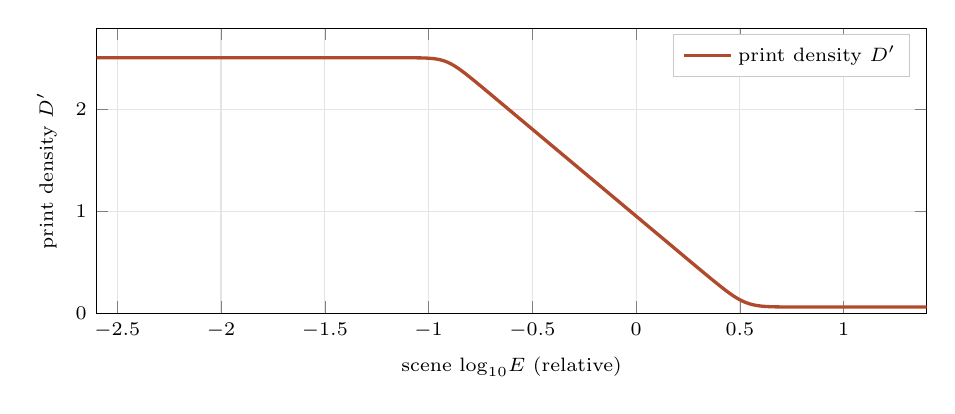
\begin{tikzpicture}
\begin{axis}[
  width=\columnwidth, height=5.2cm,
  xlabel={scene $\logE$ (relative)},
  ylabel={print density $D'$},
  xmin=-2.6, xmax=1.4, ymin=0, ymax=2.8,
  grid=both, grid style={draw=emLine!20},
  legend style={font=\scriptsize, at={(0.98,0.98)}, anchor=north east, draw=emLine!40},
  label style={font=\scriptsize}, tick label style={font=\scriptsize},
  samples=250,
]
% Composite: print curve driven by (aim - gamma_neg*(x - x0n)) as effective print logE
% Effective print logE' = k - gamma_neg*(x + 2.10)   (negative density rises with x)
\addplot[emAcc, very thick, domain=-2.6:1.4]
  {0.06 + 0.07*ln(1+exp((2.80*((1.05 - 0.61*(x+2.10)) + 0.55))/0.07))
        - 0.06*ln(1+exp((2.80*((1.05 - 0.61*(x+2.10)) + 0.55) - 2.45)/0.06))};
\addlegendentry{print density $D'$}
\end{axis}
\end{tikzpicture}
\caption{Composite scene-to-print transfer, obtained by driving \eqref{eq:printcurve} with the negative density of \eqref{eq:charcurve}. The rising left portion is scene shadow rendered as print black; the falling right portion is scene highlight rendered as print white. The soft knee at the right is the composition of the negative's shoulder with the print's toe.}
\label{fig:printcomposite}
\end{figure}

\subsection{Print Stock Profiles}

\begin{table}[htbp]
\caption{Shipping Print Stock Profiles}
\label{tab:printstocks}
\begin{center}
\renewcommand{\arraystretch}{1.15}
\begin{tabularx}{\columnwidth}{@{}l>{\raggedright\arraybackslash}X@{}}
\toprule
\textbf{Profile} & \textbf{Character} \\
\midrule
Standard 2383-type & The default. $\gamma' = 2.80$, moderate saturation, warm-leaning neutral axis, gentle toe. The reference against which everything else is judged. \\
Premium 2393-type & $\gamma' = 3.05$, higher saturation via steeper cross-terms, deeper maximum density, harder shoulder. More contrast, less latitude. \\
Fuji 3513-type & $\gamma' = 2.72$, cooler neutral axis, distinctly different green and cyan rendering, softer approach to maximum density. \\
Fuji 3521-type & $\gamma' = 2.90$, higher saturation Fuji rendering, characteristic magenta handling. \\
Bypass (scan look) & No print transfer. Negative density is inverted and normalized only. Produces the flat, low-contrast look of an unadjusted lab scan --- included deliberately, because it is what many users have actually seen and expect. \\
\bottomrule
\end{tabularx}
\end{center}
\end{table}

\subsection{Silver Retention (Bleach Bypass and ENR)}

Skipping or shortening the bleach step leaves metallic silver in the print
alongside the dye image. Silver is spectrally neutral, so the result is a
neutral density image added to the color image: contrast rises sharply,
saturation falls, and blacks become very dense.

The model is direct. Let $\bar{D}'$ be the neutral (silver) density, which is
proportional to total development:

\begin{equation}
\bar{D}' = \frac{1}{3}\sum_c \frac{D'_c - D'_{\min,c}}{\Delta D'_c} \cdot \Delta D'_{\mathrm{Ag}},
\end{equation}

and the retained-silver print density is

\begin{equation}
D'^{\mathrm{Ag}}_c = D'_c + \varrho\, \bar{D}',
\label{eq:silverretention}
\end{equation}

with $\varrho \in [0, 1]$ the retention fraction. $\varrho = 1$ is full bleach
bypass; intermediate values correspond to the ENR and ACE processes, which
retain a controlled fraction. This single scalar reproduces the entire family
of silver-retention looks, and it reproduces their characteristic property ---
that desaturation is strongest in the shadows, where $\bar{D}'$ is largest
relative to the color record --- automatically.

\subsection{Print Density to Display}

The print is viewed by transmission (projection) or reflection. In either case
the luminance reaching the eye is proportional to $10^{-D'}$, so the display
transform is

\begin{equation}
Y_c = \frac{10^{-D'_c} - 10^{-D'_{\max,c}}}{10^{-D'_{\min,c}} - 10^{-D'_{\max,c}}},
\label{eq:printtodisplay}
\end{equation}

which normalizes the print's own $\Dmin$ to display white and its $\Dmax$ to
display black. The subtraction of the $\Dmax$ term is important: without it, the
print's finite maximum density leaves a lifted black that compounds with the
display's own black level and looks washed out on an OLED panel.

The resulting linear $Y$ is converted from the print stock's primaries to
Display P3 and encoded. A viewing-condition parameter applies an optional
surround compensation exponent \cite{fairchild2013} (default $1.0$ for a phone
screen viewed in
normal room light, $0.9$ available for a simulated dark-surround projection
look).

\section{Printer Lights and the Color Science Engine}
\label{sec:printerlights}

\subsection{The Printer Light Unit}

In an optical printer, each of three channels of the printing beam is attenuated
by a calibrated filter wheel. The industry-standard increment --- the
\emph{printer point} --- is

\begin{equation}
1 \text{ point} \;=\; 0.025 \text{ in } \log_{10} \text{ exposure},
\end{equation}

so that exactly twelve points make one stop, since $12 \times 0.025 = 0.30
\approx \log_{10} 2$. Printer lights are specified as an integer triple, and a
grade is communicated between laboratory and client as three numbers such as
$(28, 25, 26)$.

\EM{} adopts this unit exactly, as an offset from the computed aim balance of
\eqref{eq:aimbalance}:

\begin{equation}
\boxed{\;\log_{10} L_c \;=\; \log_{10} L_c^{\mathrm{aim}} \;+\; 0.025\, p_c\;}
\label{eq:printerlights}
\end{equation}

with $p_c \in [-12, +12]$ integer, giving a $\pm 1$ stop range per channel. The
control is deliberately \emph{integer-valued}: printer points are integers in
practice, the quantization is finer than the visual threshold, and integer
values are what makes a grade communicable. A continuous slider here would be a
small betrayal of parameter honesty for no benefit.

\subsection{Sign Convention}

Increasing a printer light increases the exposure of the print stock in that
record, which develops more of the complementary dye, which \emph{subtracts}
that color from the print. Raising the red printer light makes the print
\emph{more cyan}, and raising all three makes the print darker.

This is counterintuitive to anyone who has used a digital color balance control,
and it is correct. \EM{} defaults to the laboratory convention and labels it
unambiguously, with the direction indicated on the control itself
(Section~\ref{sec:ui}). A preference exists to invert the sign for users who
prefer the digital convention; the underlying parameter is unchanged and
recipes remain interchangeable.

\subsection{Why Printer Lights Are Not RGB Gain}

This is the central claim of the section and the justification for exposing the
control at all.

An RGB gain applied to a display-referred image multiplies the output. A printer
light offsets the print stock's \emph{input} in log exposure, before the print
characteristic curve. Composing \eqref{eq:printerlights} with
\eqref{eq:printcurve}, the change in print density resulting from a small
printer light change is

\begin{equation}
\frac{\partial D'_c}{\partial p_c} \;=\; 0.025\;\gamma'_c(\logE'_c),
\label{eq:plsensitivity}
\end{equation}

where $\gamma'_c(\cdot)$ is the print stock's \emph{point} gamma from
\eqref{eq:pointgamma}. The sensitivity is therefore proportional to the local
slope of the print curve: large in the mid-scale, and vanishing in both the toe
and the shoulder.

The consequences are exactly the behaviors that photographers describe as
"filmic":

\begin{itemize}
\item \textbf{Color balance changes do not tint the highlights.} Near the
print's toe (scene highlights), $\gamma' \to 0$, so
$\partial D'/\partial p \to 0$. Whites stay white no matter how far the balance
is pushed. An RGB gain tints them immediately.
\item \textbf{Color balance changes do not tint the deep blacks.} The same
argument at the shoulder.
\item \textbf{The effect is strongest exactly where the eye judges color} ---
the mid-scale, skin tones, foliage.
\end{itemize}

Figure~\ref{fig:plresponse} shows the sensitivity curve. Reproducing this shape
is impossible with any pointwise gain applied after tone mapping, which is the
practical reason a print-domain model earns its complexity.

\begin{figure}[htbp]
\centering
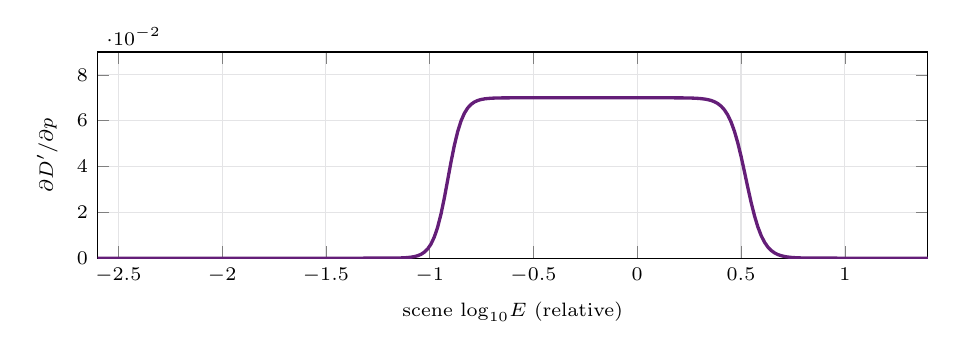
\begin{tikzpicture}
\begin{axis}[
  width=\columnwidth, height=4.2cm,
  xlabel={scene $\logE$ (relative)},
  ylabel={$\partial D' / \partial p$},
  xmin=-2.6, xmax=1.4, ymin=0, ymax=0.09,
  grid=both, grid style={draw=emLine!20},
  label style={font=\scriptsize}, tick label style={font=\scriptsize},
  samples=250,
]
\addplot[emKey, very thick, domain=-2.6:1.4]
  {0.025*2.80*( 1/(1+exp(-(2.80*((1.05 - 0.61*(x+2.10)) + 0.55))/0.07))
              - 1/(1+exp(-(2.80*((1.05 - 0.61*(x+2.10)) + 0.55) - 2.45)/0.06)) )};
\end{axis}
\end{tikzpicture}
\caption{Printer light sensitivity \eqref{eq:plsensitivity} as a function of scene exposure. Color balance authority is concentrated in the mid-scale and vanishes at both extremes. This self-protecting behavior is a property of the model, not a safeguard added on top of it.}
\label{fig:plresponse}
\end{figure}

\subsection{Density (Overall Print Exposure)}

The print exposure time $t_{\mathrm{print}}$ of \eqref{eq:printexposure} is the
lightness control, and is exposed as \emph{print density} in the same printer
point unit applied to all three channels simultaneously:

\begin{equation}
\log_{10} t_{\mathrm{print}} = 0.025\, p_{\mathrm{master}}, \quad p_{\mathrm{master}} \in [-24, +24].
\end{equation}

Increasing density darkens the print. This control replaces "brightness" and
"exposure" in the develop workspace; the capture-time exposure compensation of
\eqref{eq:anchor} remains separate and available, and the distinction between
them is real and worth teaching: exposure compensation changes where the image
sits on the \emph{negative}'s curve (affecting shadow detail and grain), while
print density changes where it sits on the \emph{print}'s curve (affecting only
the print rendering). Users discover this because the two controls genuinely
behave differently.

\subsection{Additional Color Science Controls}

Beyond printer lights, four controls operate in the print domain. Each is
defined mathematically here and mapped to its UI representation in
Table~\ref{tab:controlmap}.

\paragraph{Saturation density} Rather than a chroma multiplier, saturation is
controlled by scaling the off-diagonal terms of the printing density matrix
$\mathbf{C}$ of \eqref{eq:cmatrix}:

\begin{equation}
\mathbf{C}(\varsigma) = \mathbf{I} + \varsigma\,(\mathbf{C} - \mathbf{I}) + (1-\varsigma)\,\varpi\,\mathbf{J},
\label{eq:satdensity}
\end{equation}

where $\mathbf{J}$ is the matrix of ones scaled to preserve neutrals and
$\varsigma$ is the control. Reducing $\varsigma$ reduces the unwanted-absorption
crosstalk, \emph{increasing} apparent saturation; raising it above unity adds
crosstalk and desaturates. Because the operator lives before the print curve, its
effect is again density-dependent: saturated shadows and saturated highlights
behave differently, which a chroma multiplier cannot express.

\paragraph{Highlight roll-off} Directly modifies the print stock's toe softness
$\kappa'_t$ over $[0.5, 2.0]\times$ nominal. This is the honest control for what
other applications call "highlights."

\paragraph{Shadow lift} Modifies $\Dmax'$, which is the print's maximum density
and therefore its black level. Reducing $\Dmax'$ produces the lifted,
low-contrast black of a print made on aged paper or a flashed negative.

\paragraph{Neutral axis} A pair of parameters $(\delta_{RG}, \delta_{BG})$
applying a density-dependent tilt to the neutral axis:

\begin{equation}
D'_R \mathrel{+}= \delta_{RG}\, \psi(D'), \qquad
D'_B \mathrel{+}= \delta_{BG}\, \psi(D'),
\label{eq:neutralaxis}
\end{equation}

with $\psi(D') = (D' - \Dmin')/\Delta D' - \tfrac{1}{2}$ an antisymmetric
weighting. This is split toning expressed as an axis tilt: positive
$\delta_{RG}$ warms shadows and cools highlights simultaneously, exactly as a
tilted neutral axis in a real print does, and unlike independent
shadow/highlight tint controls it cannot produce a physically impossible
non-monotone neutral.

\subsection{Control Mapping Table}

Table~\ref{tab:controlmap} is normative. It is the authoritative translation
between the user-visible vocabulary, the internal parameter, and the equation
that consumes it. Any control added to the product must be added to this table
or it does not ship.

\begin{table}[htbp]
\caption{Control Mapping: User Term to Model Parameter}
\label{tab:controlmap}
\begin{center}
\renewcommand{\arraystretch}{1.12}
\begin{tabularx}{\columnwidth}{@{}>{\raggedright\arraybackslash}X l l@{}}
\toprule
\textbf{User control} & \textbf{Parameter} & \textbf{Eq.} \\
\midrule
Exposure compensation & $\varepsilon$ & \eqref{eq:anchor} \\
Film speed / rating & $S$ & \eqref{eq:isoshift} \\
Push / pull & $n \to A$ & \eqref{eq:activity} \\
Development time & $t/t_0$ & \eqref{eq:activity} \\
Development temperature & $T$ & \eqref{eq:activity} \\
Agitation & $a_g$ & \eqref{eq:activity} \\
Contrast index (readout) & CI & \eqref{eq:ci} \\
Coupler activity & $\|\mathbf{A}\|$ & \eqref{eq:interlayer} \\
Printer lights R/G/B & $p_R, p_G, p_B$ & \eqref{eq:printerlights} \\
Print density & $p_{\mathrm{master}}$ & \eqref{eq:printexposure} \\
Saturation density & $\varsigma$ & \eqref{eq:satdensity} \\
Highlight roll-off & $\kappa'_t$ & \eqref{eq:printcurve} \\
Shadow lift & $\Dmax'$ & \eqref{eq:printcurve} \\
Neutral axis warm/cool & $\delta_{RG}, \delta_{BG}$ & \eqref{eq:neutralaxis} \\
Silver retention & $\varrho$ & \eqref{eq:silverretention} \\
Grain amount & $g$ & \eqref{eq:grainapply} \\
Grain size & $r_g$ & \eqref{eq:grainkernel} \\
Halation threshold & $\tau$ & \eqref{eq:halsource} \\
Halation radius & $\ell$ & \eqref{eq:halpsf} \\
Halation intensity & $\alpha_h$ & \eqref{eq:haladd} \\
Halation color bias & $\boldsymbol{\beta}$ & \eqref{eq:haladd} \\
Diffusion & $w_d, \sigma_d$ & \eqref{eq:diffusion} \\
Vignetting & $v$ & \eqref{eq:vignette} \\
Chromatic aberration & $\varkappa$ & \eqref{eq:ca} \\
Barrel / pincushion & $k_1, k_2$ & \eqref{eq:distortion} \\
\bottomrule
\end{tabularx}
\end{center}
\end{table}

\section{Grain Synthesis}
\label{sec:grain}

\subsection{Grain Is Not Noise, and It Is Not a Texture}

Two failure modes dominate grain in existing products. The first overlays a
scanned grain plate, which is spatially fixed, resolution-dependent, uncoupled
to image content, and repeats visibly. The second adds Gaussian noise of
constant variance, which is uncoupled to density and has a flat spectrum,
producing something that reads as sensor noise rather than emulsion grain.

Real grain has four properties that must all be reproduced:

\begin{enumerate}
\item It is \emph{signal-dependent}: variance depends on how much of the image
was developed at that point, peaking in the mid-scale.
\item It is \emph{spatially correlated} at a scale set by the emulsion's grain
size, with a characteristic non-flat Wiener spectrum.
\item It is \emph{physically sized}: a grain is a few micrometres at the film
plane, so its appearance at a given viewing size depends on the format and the
enlargement, not on the pixel count.
\item It is \emph{chromatically structured}: in color film, the three dye
clouds form in separate layers and are essentially statistically independent,
producing colored grain; in monochrome film there is one layer, producing
neutral grain.
\end{enumerate}

\EM{} derives all four from a single generative model.

\subsection{The Filtered Poisson Model}

Model developed grains as a spatial Poisson point process. Let $\{\mathbf{p}_i\}$
be grain centers with intensity $\lambda$ (grains per unit area), and let each
grain contribute a density profile $a_i\, g(\mathbf{p} - \mathbf{p}_i)$, where
$g$ is the normalized dye cloud profile and $a_i$ is a random amplitude drawn
from the grain size distribution. The density field is the shot-noise process

\begin{equation}
D_g(\mathbf{p}) \;=\; \sum_i a_i\, g\!\left(\mathbf{p} - \mathbf{p}_i\right).
\label{eq:shotnoise}
\end{equation}

Campbell's theorem \cite{campbell1909} gives the first two moments and the power
spectrum in closed form:

\begin{align}
\mathbb{E}[D_g] &= \lambda\,\mathbb{E}[a] \int g(\mathbf{p})\, d\mathbf{p},
\label{eq:campbell-mean}\\
\mathrm{Var}[D_g] &= \lambda\,\mathbb{E}[a^2] \int g^2(\mathbf{p})\, d\mathbf{p},
\label{eq:campbell-var}\\
W(\mathbf{f}) &= \lambda\,\mathbb{E}[a^2]\, \left|G(\mathbf{f})\right|^2,
\label{eq:wiener}
\end{align}

where $G = \mathcal{F}\{g\}$ and $W$ is the Wiener (noise power) spectrum. This
is the entire theoretical content of the grain engine, and it is the reason the
model can be validated against published Wiener spectra (AC-3) rather than
tuned by eye.

\subsection{Selwyn Granularity Recovered}

Measuring density through a scanning aperture of area $A$ averages the field,
which for $A$ large compared to the grain gives

\begin{equation}
\sigma_A^2 = \frac{1}{A}\,\lambda\,\mathbb{E}[a^2] \int g^2\, d\mathbf{p},
\end{equation}

so $\sigma_A \sqrt{2A}$ is a constant of the emulsion. This is
\emph{Selwyn's law} \cite{selwyn1935}, and the constant

\begin{equation}
G_S = \sigma_A\sqrt{2A} = \sqrt{2\lambda\,\mathbb{E}[a^2]\textstyle\int g^2}
\label{eq:selwyn}
\end{equation}

is the Selwyn granularity, the quantity manufacturers publish (typically as RMS
granularity measured through a $48\,\mu$m aperture, scaled by $1000$). Because
$G_S$ is published for most stocks, \eqref{eq:selwyn} lets us fit
$\lambda\mathbb{E}[a^2]$ directly from datasheet values rather than guessing.

\subsection{Density Dependence}

A pure Poisson model predicts $\sigma^2 \propto \lambda$, and since mean density
is also $\propto \lambda$ by Nutting's relation \cite{nutting1913}

\begin{equation}
D = 0.4343\,\frac{n\,\bar{a}}{A},
\end{equation}

it predicts $\sigma \propto \sqrt{D}$, monotonically increasing. Real emulsions
do not behave this way at high density: as development approaches completion the
available crystals are exhausted, grain overlap saturates, and granularity
falls again.

The correct model replaces the Poisson count with a \emph{binomial} count: there
are $N$ crystals available, and each develops with probability $p$ determined by
exposure. Then $\mathrm{Var}[n] = Np(1-p)$ and

\begin{equation}
\boxed{\;\sigma_D^2(D) \;=\; \sigma_{\mathrm{ref}}^2 \cdot \frac{p(1-p)}{p_{\mathrm{ref}}(1-p_{\mathrm{ref}})}\;}
\qquad p = \frac{D - \Dmin}{\Delta D}
\label{eq:grainvar}
\end{equation}

with $p_{\mathrm{ref}} = 0.5$ so the reference is the peak. This recovers the
observed inverted-U granularity--density relationship with no free parameters
beyond the peak magnitude.

A shape exponent pair $(\nu_1, \nu_2)$ generalizes \eqref{eq:grainvar} to
$\sigma_D^2 \propto p^{\nu_1}(1-p)^{\nu_2}$ for stocks whose measured curve is
asymmetric; monochrome stocks typically fit $(\nu_1, \nu_2) = (1.0, 0.45)$,
which rises to a peak at $p \approx 0.69$ and falls only modestly thereafter,
matching black-and-white behavior.

\begin{figure}[htbp]
\centering
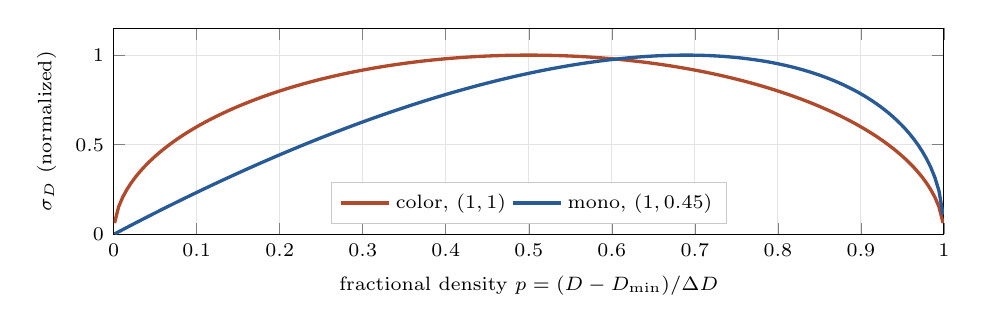
\begin{tikzpicture}
\begin{axis}[
  width=\columnwidth, height=4.2cm,
  xlabel={fractional density $p = (D-\Dmin)/\Delta D$},
  ylabel={$\sigma_D$ (normalized)},
  xmin=0, xmax=1, ymin=0, ymax=1.15,
  grid=both, grid style={draw=emLine!20},
  legend style={font=\scriptsize, at={(0.5,0.05)}, anchor=south, draw=emLine!40, legend columns=2},
  label style={font=\scriptsize}, tick label style={font=\scriptsize},
  samples=200,
]
\addplot[emAcc, very thick, domain=0.001:0.999] {sqrt(4*x*(1-x))};
\addlegendentry{color, $(1,1)$}
\addplot[emBlue, very thick, domain=0.001:0.999] {(x^1.0 * (1-x)^0.45)/ (0.69^1.0 * 0.31^0.45)};
\addlegendentry{mono, $(1,0.45)$}
\end{axis}
\end{tikzpicture}
\caption{Granularity versus density from \eqref{eq:grainvar}. Grain vanishes in clear film and in fully developed maximum density, and peaks in the mid-scale --- which is why grain is most visible in skies and skin, not in shadows.}
\label{fig:grainvar}
\end{figure}

\subsection{The Grain Kernel and Clustering}

The dye cloud profile $g$ is modelled as a mixture of two Gaussians, capturing
both the individual grain and the tendency of grains to cluster:

\begin{equation}
g(\mathbf{p}) = (1-\chi)\, \mathcal{N}(\mathbf{p};\, \sigma_1) + \chi\, \mathcal{N}(\mathbf{p};\, \sigma_2),
\qquad \sigma_2 = \zeta \sigma_1,
\label{eq:grainkernel}
\end{equation}

with $\chi \in [0, 0.4]$ the clustering fraction and $\zeta \approx 3$. Since the
Fourier transform of a Gaussian is a Gaussian, the Wiener spectrum follows in
closed form from \eqref{eq:wiener}:

\begin{equation}
W(f) = \lambda \mathbb{E}[a^2]\left[(1-\chi)e^{-2\pi^2\sigma_1^2 f^2} + \chi e^{-2\pi^2\sigma_2^2 f^2}\right]^2 .
\label{eq:wienerclosed}
\end{equation}

Equation \eqref{eq:wienerclosed} is what AC-3 compares against measured
data. Fitting a stock is therefore a two-parameter least-squares problem in
$(\sigma_1, \chi)$ against its published Wiener spectrum, with $\lambda
\mathbb{E}[a^2]$ pinned by the published RMS granularity through
\eqref{eq:selwyn}. This is a genuine fit to measurement, satisfying the
"defaults are measurements" principle of Section~\ref{sec:intro-thesis}.

\subsection{Format Scaling}
\label{sec:formatscale}

All grain geometry is specified in micrometres at the film plane. The
conversion to render pixels is

\begin{equation}
\sigma^{\mathrm{px}} = \sigma^{\mu\mathrm{m}} \cdot \frac{W_{\mathrm{px}}}{1000\, W_{\mathrm{mm}}},
\label{eq:formatscale}
\end{equation}

where $W_{\mathrm{px}}$ is the render width in pixels and $W_{\mathrm{mm}}$ the
simulated frame width in millimetres. A \emph{format} selector supplies
$W_{\mathrm{mm}}$: $36$\,mm for 135, $56$\,mm for 645/6$\times$6, $102$\,mm for
4$\times$5, $24.9$\,mm for Super\,35, $12.5$\,mm for Super\,16, $10.3$\,mm for
8\,mm. Selecting Super\,16 makes the grain of the same emulsion roughly three
times larger relative to the frame, which is exactly the real relationship and
requires no separate "grain size" authoring per format.

The same equation governs $\sigma_1, \sigma_2$ of the interlayer model
\eqref{eq:twoscale} and the halation scattering length \eqref{eq:halpsf}, so
format selection coherently rescales every spatial phenomenon at once. This is
a significant structural advantage of specifying everything in physical units.

\subsection{Resolution Independence and Determinism}

NFR-08 requires that identical parameters produce identical output, and the
preview/export equivalence of NFR-07 requires that the grain \emph{structure} be
the same field sampled at two resolutions, not two different random fields.

Both are achieved by defining the noise on a lattice in \emph{film-plane
coordinates} rather than pixel coordinates, the same device that makes
stochastic grain models resolution-independent \cite{newson2017}. For a render pixel at position
$\mathbf{q}$ pixels, the film coordinate is $\mathbf{m} = \mathbf{q} \cdot
1000\,W_{\mathrm{mm}} / W_{\mathrm{px}}$ in micrometres. The white noise field is
evaluated by hashing the integer lattice cell of $\mathbf{m}$ at the grain
lattice pitch, so:

\begin{itemize}
\item The same film position yields the same random value at every render
resolution.
\item Preview at $1/4$ resolution samples the same field more coarsely, which
--- through \eqref{eq:formatscale} --- correctly reduces the per-pixel variance
according to Selwyn's law. The preview grain therefore looks like the export
grain viewed at preview size, which is what WYSIWYG actually means here.
\item Changing the frame seed changes the hash salt, producing an independent
realization, so "re-roll grain" is a one-integer operation.
\end{itemize}

\subsection{Chromatic Structure}

In color film the three dye clouds form in physically separate layers from
independent crystal populations, so the three noise fields are close to
statistically independent, producing visibly colored grain. In monochrome film
there is a single silver image, so the three output channels receive the
identical field, producing neutral grain.

\EM{} interpolates between these through a correlation matrix
$\mathbf{R}$ with unit diagonal and off-diagonal $\varphi$:

\begin{equation}
\mathbf{n} = \mathbf{L}\, \mathbf{z}, \qquad \mathbf{L}\mathbf{L}^\top = \mathbf{R},
\label{eq:graincorr}
\end{equation}

where $\mathbf{z}$ is a vector of three independent standard normal fields and
$\mathbf{L}$ is the Cholesky factor, computed once on the host. Setting
$\varphi = 0$ gives fully chromatic grain, $\varphi = 1$ gives neutral grain,
and the shipping defaults are $\varphi \approx 0.15$ for color negative,
$\varphi \approx 0.35$ for transparency (whose layers are more closely coupled),
and $\varphi = 1$ for monochrome.

Because $\mathbf{R}$ is a $3\times3$ correlation matrix, its Cholesky factor is
lower triangular with six nonzero entries, so \eqref{eq:graincorr} costs six
multiply-adds.

\subsection{Application to Density}

The grain field is added in the density domain, scaled by the density-dependent
standard deviation:

\begin{equation}
\boxed{\;\hat{D}_c(\mathbf{p}) \;=\; D_c(\mathbf{p}) \;+\; g \cdot \sigma_{D,c}\!\left(D_c(\mathbf{p})\right) \cdot n_c(\mathbf{p})\;}
\label{eq:grainapply}
\end{equation}

with $g$ the user's grain amount ($0$ to $2$, default $1$; $1$ means "the
physically correct amount for this stock"). Setting $g = 0$ produces a
grainless render, which is not physical but is a legitimate user choice; the UI
labels the $g = 1$ position on the slider explicitly.

Note that grain is added to the \emph{negative} density, which is then printed
through \eqref{eq:printcurve}. The print stock's gamma of $2.8$ therefore
amplifies negative grain by that factor in the print, and the print's toe and
shoulder \emph{suppress} grain in print highlights and print blacks. Both are
correct, both are free, and neither is achievable by adding grain to the final
image.

\subsection{Generation Algorithm}

Two synthesis modes are required, selected by the expected number of grains per
render pixel $\Lambda = \lambda\,\Delta A_{\mathrm{px}}$:

\begin{itemize}
\item \textbf{Gaussian mode} ($\Lambda \geq 10$). The central limit theorem
applies; generate a white Gaussian field and convolve with $g$. This is the
common case at full resolution.
\item \textbf{Poisson mode} ($\Lambda < 10$). The Gaussian approximation fails
and produces grain that is too smooth and insufficiently "clumpy"; individual
grains must be realized. This occurs for large formats rendered small, and for
heavily enlarged small formats. The shader draws $n \sim \mathrm{Poisson}(\Lambda)$
per lattice cell using Knuth's method \cite{knuth1997} (acceptable since
$\Lambda$ is small) and splats.
\end{itemize}

\begin{lstlisting}[language=Metal, caption={Deterministic hash and grain field generation (Gaussian mode).}, label={lst:grain}]
// PCG-style integer hash: deterministic, well-distributed, cheap.
inline uint pcg_hash(uint v) {
    uint state = v * 747796405u + 2891336453u;
    uint word  = ((state >> ((state >> 28u) + 4u)) ^ state) * 277803737u;
    return (word >> 22u) ^ word;
}
inline float hash01(uint3 c, uint salt) {
    uint h = pcg_hash(c.x ^ pcg_hash(c.y ^ pcg_hash(c.z ^ salt)));
    return float(h) * 2.3283064365386963e-10f;   // 1/2^32
}
// Box-Muller from two hashed uniforms; returns standard normal.
inline float gauss(uint3 c, uint salt) {
    float u1 = max(hash01(c, salt),        1e-7f);
    float u2 =     hash01(c, salt ^ 0x9E3779B9u);
    return sqrt(-2.0f * log(u1)) * cos(6.2831853f * u2);
}

kernel void grain_white_field(
    texture2d<float, access::write> outTex [[texture(0)]],
    constant GrainParams&           P      [[buffer(0)]],
    uint2 gid [[thread_position_in_grid]])
{
    if (gid.x >= outTex.get_width() || gid.y >= outTex.get_height()) return;

    // Map pixel -> film-plane micrometres -> grain lattice cell.
    // P.umPerPixel = 1000 * frameWidthMM / renderWidthPX
    float2 um   = float2(gid) * P.umPerPixel;
    int2   cell = int2(floor(um / P.latticePitchUM));

    float3 z;
    for (uint c = 0; c < 3; ++c)
        z[c] = gauss(uint3(uint2(cell), c), P.seed);

    // Correlate the three records via the Cholesky factor of R.
    float3 n;
    n.x = P.L00 * z.x;
    n.y = P.L10 * z.x + P.L11 * z.y;
    n.z = P.L20 * z.x + P.L21 * z.y + P.L22 * z.z;

    outTex.write(float4(n, 1.0f), gid);
}
\end{lstlisting}

The white field is then convolved with the two-Gaussian kernel of
\eqref{eq:grainkernel} using the separable recursive filter of
Section~\ref{sec:recursive-blur}, and combined with the density image by
\eqref{eq:grainapply}. Total cost is two separable blur passes plus two
pointwise passes over a single-precision RGBA texture.

\subsection{A Note on Downsampling}

If a full-resolution render is exported and then downsampled by an external
tool, the grain will be averaged and its variance reduced by the sampling
area --- correctly, per Selwyn. If instead the user exports at a reduced
resolution, \EM{} renders at that resolution and \eqref{eq:formatscale} gives
smaller pixel-space grain, again correctly. The two paths agree to within
the difference between the resampling filter and the grain kernel, which is
below visual threshold. This consistency is verified by test V-11 in
Section~\ref{sec:validation}.

\section{Halation}
\label{sec:halation}

\subsection{Physical Origin}

Light entering the emulsion is not entirely absorbed. Some fraction traverses
all three sensitized layers, enters the transparent base, and is redirected back
into the emulsion by two distinct mechanisms:

\begin{enumerate}
\item \textbf{Base reflection.} At the base--air interface on the rear surface,
rays striking at angles beyond the critical angle
$\theta_c = \arcsin(1/n)$ are totally internally reflected. Having crossed the
base twice, they re-enter the emulsion displaced by
\begin{equation}
r = 2\, t_b \tan\theta,
\label{eq:ringradius}
\end{equation}
where $t_b$ is base thickness. Because only $\theta > \theta_c$ reflects
totally, the returned energy forms an \emph{annulus} of inner radius
$r_{\min} = 2 t_b \tan\theta_c$, not a disc. For a $125\,\mu$m acetate base with
$n = 1.50$, $\theta_c = 41.8^\circ$ and $r_{\min} \approx 224\,\mu$m --- roughly
$0.6\%$ of the width of a 135 frame, which is a visible ring.
\item \textbf{Diffuse scattering.} Light scatters from silver halide crystals
and from layer interfaces, producing a monotone, heavy-tailed spread with no
characteristic ring.
\end{enumerate}

Modern films carry an antihalation undercoat or a rem-jet backing that absorbs
most light reaching the base, suppressing the ring almost entirely and leaving
the diffuse component. \EM{} models both and lets the stock profile weight
them, because the ring is exactly what makes certain older stocks and certain
motion picture negatives look the way they do, while the diffuse component is
what modern stocks exhibit.

\subsection{Wavelength Dependence}

Halation is strongly red-biased, for two compounding reasons. First, the
red-sensitive layer sits deepest in the stack, so returning light passes through
it first and most strongly. Second, longer wavelengths are absorbed less by the
emulsion and by the antihalation layer, so more red light survives the round
trip. The result is that the characteristic halo around a bright highlight is
orange-red, and this is the single most recognizable film cue in the entire
pipeline.

Scattering lengths therefore satisfy $\ell_R > \ell_G > \ell_B$, with typical
ratios $\ell_R : \ell_G : \ell_B \approx 1.00 : 0.62 : 0.44$, and channel
weights $\boldsymbol{\beta} \approx (1.00, 0.42, 0.22)$.

\subsection{The Source Term}

Halation is driven by scene exposure above a threshold, evaluated in the
\emph{linear scene-referred domain} before the characteristic curve, per the
ordering derivation of Section~\ref{sec:arch}. A hard threshold
$\max(0, E - \tau)$ has a discontinuous derivative and produces a visible
contour where the halo begins. \EM{} reuses the softplus primitive of
\eqref{eq:softplus}:

\begin{equation}
\boxed{\;S(\mathbf{p}) \;=\; \left[\softp{\kappa_h}{E_Y(\mathbf{p}) - \tau}\right]^{\,q}\;}
\label{eq:halsource}
\end{equation}

where $E_Y$ is the luminance-weighted exposure, $\tau$ is the threshold in
relative exposure units (default $\tau = 1.6$, i.e. about $3.2$ stops above
middle gray), $\kappa_h$ is the knee softness (default $0.15$), and $q$ is the
source exponent (default $1.0$; $q = 2$ concentrates the effect into the very
brightest sources, which suits point highlights such as street lamps).

Using luminance rather than per-channel exposure is deliberate: the source of the
scattered light is the total radiance at that point, and the channel dependence
enters through the transport, not the source. Per-channel thresholding produces
colored source regions and looks wrong.

\subsection{The Point Spread Function}

The diffuse component is modelled with a normalized isotropic exponential:

\begin{equation}
\boxed{\;h_\ell(r) \;=\; \frac{1}{2\pi \ell^2}\, e^{-r/\ell}, \qquad \int_{\Rspace^2} h_\ell \, dA = 1\;}
\label{eq:halpsf}
\end{equation}

whose two-dimensional Fourier transform is available in closed form,

\begin{equation}
H_\ell(f) \;=\; \left[1 + (2\pi \ell f)^2\right]^{-3/2}.
\label{eq:halotf}
\end{equation}

Equation \eqref{eq:halotf} is what makes the model verifiable: it is the optical
transfer function of the scattering layer, and it can be compared directly
against a measured MTF degradation or against the radial profile of a
photographed point source (AC-4).

The exponential is chosen over a Gaussian because it is heavy-tailed. A Gaussian
halo has a definite edge; an exponential halo has a bright core and a long,
faint skirt, which is what the eye reads as "glow inside the film" rather than
"blur applied to the highlights." This distinction is perceptually decisive and
costs nothing to get right.

The ring component uses

\begin{equation}
h^{\mathrm{ring}}(r) \;=\; \frac{1}{Z}\exp\!\left[-\frac{(r - r_{\min})^2}{2 w_r^2}\right],
\label{eq:halring}
\end{equation}

with $r_{\min}$ from \eqref{eq:ringradius}, $w_r$ the ring width set by the
angular spread, and $Z$ the normalization $\int h^{\mathrm{ring}} dA = 1$. The
composite PSF is

\begin{equation}
h(r) = (1 - \omega)\, h_\ell(r) + \omega\, h^{\mathrm{ring}}(r),
\end{equation}

with $\omega$ the base-reflection weight, near zero for modern stocks and up to
$0.35$ for stocks without effective antihalation.

\subsection{Recombination and Energy Conservation}

The scattered light must be added to the direct exposure --- and, strictly,
removed from it, since it is the same photons. The energy-conserving form is

\begin{equation}
\boxed{\;E'_c \;=\; \left(1 - \alpha_h \beta_c\right) E_c \;+\; \alpha_h \beta_c \left(h_{\ell_c} * S\right)\;}
\label{eq:haladd}
\end{equation}

where $\alpha_h$ is the halation intensity ($0$ to $1$, default $0.18$) and
$\beta_c$ the channel bias. Because $\int h = 1$, \eqref{eq:haladd} preserves
total energy exactly when $S = E_c$, and the attenuation term correctly darkens
the core of an extremely bright highlight as its energy is redistributed
outward. Omitting the attenuation term --- as an additive glow does --- inflates
total scene energy and makes strong halation settings brighten the entire image,
a defect that manifests as "the halation slider is also an exposure slider."

\begin{figure}[htbp]
\centering
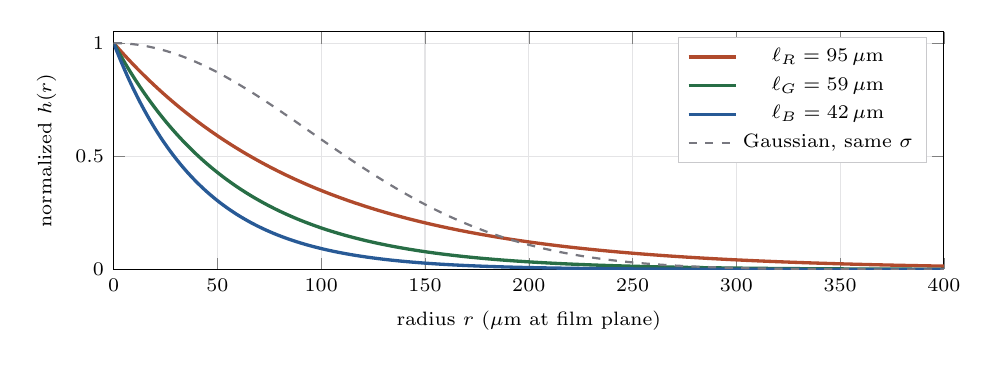
\begin{tikzpicture}
\begin{axis}[
  width=\columnwidth, height=4.6cm,
  xlabel={radius $r$ ($\mu$m at film plane)},
  ylabel={normalized $h(r)$},
  xmin=0, xmax=400, ymin=0, ymax=1.05,
  grid=both, grid style={draw=emLine!20},
  legend style={font=\scriptsize, at={(0.98,0.98)}, anchor=north east, draw=emLine!40},
  label style={font=\scriptsize}, tick label style={font=\scriptsize},
  samples=250,
]
\addplot[emAcc, very thick, domain=0:400] {exp(-x/95)};
\addlegendentry{$\ell_R = 95\,\mu$m}
\addplot[emGreen, very thick, domain=0:400] {exp(-x/59)};
\addlegendentry{$\ell_G = 59\,\mu$m}
\addplot[emBlue, very thick, domain=0:400] {exp(-x/42)};
\addlegendentry{$\ell_B = 42\,\mu$m}
\addplot[emLine, thick, dashed, domain=0:400] {exp(-(x*x)/(2*95*95))};
\addlegendentry{Gaussian, same $\sigma$}
\end{axis}
\end{tikzpicture}
\caption{Halation point spread functions. The dashed Gaussian falls to negligible values by $250\,\mu$m; the exponential retains a visible skirt far beyond. That skirt is the visual signature of halation and is why a Gaussian bloom does not read as film.}
\label{fig:halpsf}
\end{figure}

\subsection{Real-Time Evaluation}
\label{sec:recursive-blur}

A direct convolution with $h_\ell$ at $\ell = 95\,\mu$m on a 48\,MP render
corresponds to a kernel radius of roughly $150$ pixels, which is
$\sim\!70{,}000$ taps per pixel. This is not viable. Three strategies were
evaluated.

\paragraph{FFT convolution} Exact and $O(N \log N)$, but requires two complex
transforms of a 48\,MP image, which exceeds the memory budget of NFR-03 and is
awkward to tile.

\paragraph{Recursive IIR filtering} A separable first-order recursive filter
realizes $e^{-|x|/\ell}$ exactly in one dimension at $O(1)$ per pixel. Applied
separably it produces $e^{-(|x|+|y|)/\ell}$, which is not isotropic --- it has
visible diamond-shaped anisotropy that is objectionable on point highlights.
Deriche's third-order approximation \cite{deriche1993,young1995} improves
isotropy but not enough at these radii.

\paragraph{Fitted mip pyramid (chosen)} The isotropic exponential is
approximated as a weighted sum of Gaussians,

\begin{equation}
h_\ell(r) \;\approx\; \sum_{j=1}^{J} w_j\, \mathcal{N}\!\left(r;\, s_j \ell\right),
\qquad \sum_j w_j = 1,
\label{eq:gaussmix}
\end{equation}

each of which is separable, isotropic, and --- critically --- can be evaluated
at a mip level chosen so that its kernel is only a few pixels wide. With $J = 4$
levels spaced by factors of four in $\sigma$, the frequency-domain fit of
\eqref{eq:gaussmix} to \eqref{eq:halotf} has a maximum relative error below
$3\%$ over $[0, 1/(2\ell)]$, which is far below AC-4 tolerance.

The coefficients $(w_j, s_j)$ are produced by an offline least-squares fit in the
frequency domain, stored in the stock profile, and regenerated by the profile
authoring tool whenever the target PSF changes. Representative values for the
$J = 4$ fit are given in Table~\ref{tab:gaussmix}.

\begin{table}[htbp]
\caption{Representative Gaussian Mixture Fit to \eqref{eq:halotf}}
\label{tab:gaussmix}
\begin{center}
\renewcommand{\arraystretch}{1.15}
\begin{tabular}{@{}lccc@{}}
\toprule
\textbf{Term $j$} & $s_j$ ($\times\ell$) & $w_j$ & \textbf{Mip level} \\
\midrule
1 & $0.42$ & $0.451$ & 0 \\
2 & $1.15$ & $0.318$ & 1 \\
3 & $3.30$ & $0.163$ & 3 \\
4 & $9.60$ & $0.068$ & 5 \\
\bottomrule
\multicolumn{4}{@{}p{0.92\columnwidth}@{}}{\footnotesize Produced by the offline frequency-domain fitter; regenerate rather than hand-edit. Mip level is chosen so each Gaussian has $\sigma \le 3$ pixels at that level.}
\end{tabular}
\end{center}
\end{table}

The resulting pass structure is: build a five-level pyramid of the source term
$S$ by successive $2\times$ box-plus-tent downsamples; apply a small separable
Gaussian at each retained level; upsample with bilinear filtering and accumulate
with weights $w_j$; combine per \eqref{eq:haladd}. Total cost is approximately
$1.33\times$ the base-resolution pass count due to the geometric series, and the
memory overhead is one-third of a full-resolution single-channel texture.

The ring component, when $\omega > 0$, is evaluated on the level-3 pyramid tap
using a small annular kernel of 16 taps arranged on a Poisson-disc ring, since
the ring is spatially large but the mip level makes it only a few pixels wide.

\subsection{Parameter Summary}

\begin{table}[htbp]
\caption{Halation Parameters}
\label{tab:halparams}
\begin{center}
\renewcommand{\arraystretch}{1.15}
\begin{tabularx}{\columnwidth}{@{}ll>{\raggedright\arraybackslash}X@{}}
\toprule
\textbf{Symbol} & \textbf{Default} & \textbf{Meaning} \\
\midrule
$\tau$        & $1.6$   & Threshold, relative exposure \\
$\kappa_h$    & $0.15$  & Threshold knee softness \\
$q$           & $1.0$   & Source exponent \\
$\ell_R$      & $95\,\mu$m & Red scattering length \\
$\ell_G/\ell_R$ & $0.62$ & Green ratio \\
$\ell_B/\ell_R$ & $0.44$ & Blue ratio \\
$\alpha_h$    & $0.18$  & Intensity \\
$\boldsymbol{\beta}$ & $(1.0, 0.42, 0.22)$ & Channel bias \\
$\omega$      & $0.05$  & Base-reflection ring weight \\
$t_b$         & $125\,\mu$m & Base thickness (drives $r_{\min}$) \\
\bottomrule
\end{tabularx}
\end{center}
\end{table}

The user-facing controls are threshold, radius (a multiplier on $\ell_R$ with the
ratios held fixed), intensity, and color bias (a single warm--cool parameter that
moves $\boldsymbol{\beta}$ along a locus rather than exposing three channels).
The remaining parameters live in the stock profile.

\section{Optical Simulation}
\label{sec:optical}

\subsection{The Placement Problem}

Lens artifacts belong to the taking lens and therefore occur \emph{before} the
film is exposed. Diffusion filters, however, may sit on the taking lens or may
be a property of the projection and viewing chain, and bloom in a projected
print is a property of the projector and the screen. \EM{} therefore splits the
optical stage into two passes at different points in the pipeline:

\begin{itemize}
\item \textbf{Pre-exposure optics} (before \eqref{eq:charcurve}): geometric
distortion, vignetting, chromatic aberration, and taking-lens diffusion. These
modify the exposure that forms the latent image, so they interact correctly with
the characteristic curve --- a vignetted corner falls further down the toe and
loses shadow detail, which is what actually happens.
\item \textbf{Post-print optics} (after \eqref{eq:printtodisplay}): bloom and
veiling glare associated with viewing. These act on the rendered image.
\end{itemize}

Applications that apply all optical effects at the end get vignetting
qualitatively wrong: a post-hoc darkening multiplies the output, whereas a real
vignette reduces exposure and therefore changes contrast and color in the
corners, not merely brightness.

\subsection{Geometric Distortion}

The Brown--Conrady model is used, with radial and tangential terms. For a
normalized image coordinate $\mathbf{x} = (x, y)$ measured from the optical
center with $r^2 = x^2 + y^2$:

\begin{align}
\mathbf{x}_d &= \mathbf{x}\left(1 + k_1 r^2 + k_2 r^4 + k_3 r^6\right) \nonumber \\
&\quad + \begin{pmatrix} 2 p_1 x y + p_2 (r^2 + 2x^2) \\ p_1 (r^2 + 2y^2) + 2 p_2 x y \end{pmatrix}.
\label{eq:distortion}
\end{align}

$k_1 < 0$ gives barrel distortion, $k_1 > 0$ pincushion. The tangential terms
$p_1, p_2$ model decentering and are exposed only in the "vintage lens" presets,
where a small asymmetry is a large part of the character.

Distortion is implemented as an inverse warp: for each output pixel, compute the
source coordinate and sample with a Catmull--Rom kernel. Forward warping would
require scatter and produce holes. Note that Apple's lens correction is
\emph{enabled} at decode (Listing~\ref{lst:rawconfig}), so the input is
rectilinear and \eqref{eq:distortion} adds the simulated lens's distortion to a
clean base rather than fighting the phone lens's own.

\subsection{Vignetting}

Two mechanisms are modelled and summed in the illumination domain.

\paragraph{Natural (cos-fourth) falloff} An unavoidable consequence of the
geometry of an ideal lens:

\begin{equation}
V_{\mathrm{nat}}(\theta) = \cos^4 \theta, \qquad \tan\theta = \frac{r\, d}{f},
\end{equation}

where $d$ is half the frame diagonal and $f$ the focal length. Selecting a
shorter simulated focal length therefore automatically produces stronger
falloff, which is correct and which links the vignette control to the format
and lens selection rather than leaving it free-floating.

\paragraph{Mechanical vignetting} Aperture obstruction by the lens barrel,
which is strongly aperture-dependent and vanishes on stopping down:

\begin{equation}
V_{\mathrm{mech}}(r) = 1 - v\,\max\!\left(0, \frac{r - r_0}{1 - r_0}\right)^{\!\eta} \cdot \varsigma_N,
\end{equation}

with $\varsigma_N = \mathrm{clamp}\!\left((N_{\max}/N)^2, 0, 1\right)$ the
aperture dependence, $N$ the f-number, $r_0$ the onset radius, and $\eta$ the
falloff exponent (default $2.2$). The combined operator is

\begin{equation}
\boxed{\;E' = E \cdot V_{\mathrm{nat}}\cdot V_{\mathrm{mech}}\;}
\label{eq:vignette}
\end{equation}

applied to linear exposure, pre-characteristic-curve.

\subsection{Chromatic Aberration}

Lateral chromatic aberration is a wavelength-dependent magnification. It is
modelled as a per-channel radial scale about the optical center:

\begin{equation}
\mathbf{x}_c = \mathbf{x}\left(1 + \varkappa\, \delta_c\, r^2\right),
\qquad \boldsymbol{\delta} = (+1, 0, -1),
\label{eq:ca}
\end{equation}

so the red and blue records are scaled oppositely and the green record is the
reference. $\varkappa$ is the aberration strength. The quadratic $r^2$
dependence rather than a constant scale is important: real lateral CA is
negligible at the center and grows toward the corners, and a constant scale
produces visible fringing on center subjects where there should be none.

Longitudinal chromatic aberration --- the shift of focal plane with wavelength,
which produces the green/magenta fringing on out-of-focus edges --- requires
depth information and is implemented only when a depth map is available from
capture, as a per-channel defocus radius offset.

\subsection{Diffusion Filters}

A diffusion filter (Pro-Mist, Hollywood Black Magic, and similar) contains
particles that scatter a small fraction of the light over a wide angle. The
visible effects are a soft halo around highlights and, characteristically, a
lifting of shadows \emph{adjacent to} highlights --- a local, not global, black
lift. Modelling it as a global blur-and-blend loses that locality and simply
looks out of focus.

The model is a two-term veiling glare:

\begin{equation}
\boxed{\;E' = (1 - w_d) E \;+\; w_d \left[(1-\varrho_d)\, G_{\sigma_1} * E \;+\; \varrho_d\, G_{\sigma_2} * E\right]\;}
\label{eq:diffusion}
\end{equation}

with $\sigma_1$ small (a few pixels, the tight halo), $\sigma_2$ very large (the
broad veil), $\varrho_d$ the split, and $w_d$ the filter strength ($1/8$, $1/4$,
$1/2$, $1$, $2$ presets mapping to $w_d \in \{0.03, 0.06, 0.11, 0.19, 0.30\}$).
Because the operation is in linear exposure, a bright highlight contributes far
more to the veil than a mid-tone, which localizes the effect around highlights
automatically --- the essential behavior, obtained without a threshold.

Diffusion is applied \emph{pre-exposure} when the user selects "taking lens
filter" and \emph{post-print} when they select "projection glare." The two look
meaningfully different: pre-exposure diffusion is compressed by the film's
shoulder and looks restrained; post-print diffusion is not and looks stronger.
Both are offered, and the difference is a small piece of photographic education
delivered by a toggle.

\subsection{Bloom}

Bloom is the post-print counterpart of halation: the spread of very bright areas
in the viewing chain. It uses the same pyramid machinery as
Section~\ref{sec:recursive-blur} with a Gaussian rather than exponential target
and a higher threshold, and is applied to display-linear values. It is disabled
by default, since halation already supplies the film-side glow and stacking both
is a common way to make an image look cheap.

\subsection{Depth-Dependent Effects}

When the capture provides a depth map (available on devices with a LiDAR
scanner or through the dual-camera disparity estimate), three additional effects
become available:

\paragraph{Synthetic defocus} A depth-varying circle of confusion,
\begin{equation}
c(z) = \frac{f^2}{N\,(z_f - f)}\cdot\frac{|z - z_f|}{z},
\end{equation}
with $z_f$ the focus distance. Gathered with a scatter-as-gather approach at
half resolution.

\paragraph{Cat-eye (optical vignetting) bokeh} Off-axis bokeh discs are
truncated by the lens barrel, producing the characteristic lemon shape. The
aperture shape at image radius $r$ is the intersection of two circles of radius
$R$ whose centers are separated by $\varsigma_{\mathrm{cat}}\, r$; the sampling
kernel is masked by that intersection, oriented along the radial direction.

\paragraph{Aperture blade shape} An $n$-gon mask with optional blade curvature,
producing polygonal bokeh for $n \le 9$.

These are marked SHOULD (FR-10) rather than MUST, since depth is not available
for imported files and the quality of phone depth maps at object boundaries is
the limiting factor rather than the optical model.

\subsection{Deferred: Lens Breathing}

Lens breathing --- the change of field of view with focus --- is a temporal
phenomenon with no meaning for a single still frame. It is listed in the
original proposal and is correctly deferred to the video release, where it will
be implemented as a focus-driven scale animation applied before distortion. It
is recorded here so that the omission from v1.0 is deliberate and documented
rather than an oversight.

\subsection{Cost Summary}

\begin{table}[htbp]
\caption{Optical Stage Costs at 12\,MP}
\label{tab:opticalcost}
\begin{center}
\renewcommand{\arraystretch}{1.15}
\begin{tabular}{@{}lll@{}}
\toprule
\textbf{Effect} & \textbf{Passes} & \textbf{Cost} \\
\midrule
Distortion + CA (fused)  & 1 warp    & $1.0\times$ base \\
Vignetting               & fused     & negligible \\
Diffusion                & pyramid   & $1.4\times$ base \\
Bloom                    & pyramid   & $1.4\times$ base \\
Synthetic defocus        & 3 (half)  & $1.1\times$ base \\
\bottomrule
\end{tabular}
\end{center}
\end{table}

Distortion, chromatic aberration, and vignetting are fused into a single warp
kernel: the kernel computes the distorted coordinate once, applies the
per-channel CA scale to it, performs three filtered samples, and multiplies by
the vignette factor. Three separate passes would cost three full-resolution
round trips to memory for no benefit.

\section{Aging, Damage, and Imperfection}
\label{sec:aging}

\subsection{Design Stance}

This stage is the one most likely to make the product look cheap, and it is
therefore governed by a stricter rule than the rest of the pipeline: \emph{every
artifact must be off by default, must be physically parameterized, and must be
capable of subtlety}. The failure mode of consumer film apps is not that they
have light leaks; it is that their light leaks are a fixed PNG at fixed opacity
in a fixed corner.

Two structural decisions follow. First, all artifacts are procedural and seeded,
so they never repeat across frames. Second, all artifacts are applied in the
domain where the corresponding physical damage occurs, which for most of them is
the negative, not the print --- meaning a scratch in the negative prints
\emph{light}, not dark, and dust on the negative prints as white specks. Getting
this polarity right is a small detail that separates a considered
implementation from a texture overlay, since almost every consumer application
renders dust as dark.

\subsection{Artifact Taxonomy and Domain}

\begin{table}[htbp]
\caption{Aging Artifacts, Domain, and Polarity}
\label{tab:aging}
\begin{center}
\renewcommand{\arraystretch}{1.15}
\begin{tabularx}{\columnwidth}{@{}l l l >{\raggedright\arraybackslash}X@{}}
\toprule
\textbf{Artifact} & \textbf{Domain} & \textbf{Polarity} & \textbf{Mechanism} \\
\midrule
Dust           & neg. $D$   & $+D$ & Opaque particle blocks printing light; prints white. \\
Scratch (emulsion) & neg. $D$ & $-D$ & Emulsion removed; prints dark. \\
Scratch (base) & neg. $D$   & $+D$ & Base abraded, scatters; prints light. \\
Chemical streak & neg. $D$  & $\pm D$ & Uneven development; direction-aligned. \\
Edge fog       & lin. $E$   & $+E$ & Light leaked at the edges pre-development. \\
Light leak     & lin. $E$   & $+E$ & Broad exposure through a body seam. \\
Halide fog     & neg. $\Dmin$ & $+\Dmin$ & Age/heat/radiation; raises base fog. \\
Expired shift  & $\theta$   & --- & Differential layer speed and gamma loss. \\
Frame jitter   & geometry   & --- & Registration error in transport. \\
Gate weave     & geometry   & --- & Low-frequency lateral drift (video only). \\
\bottomrule
\end{tabularx}
\end{center}
\end{table}

\subsection{Expired Film}

The most rewarding of these to model correctly, because it is entirely a
parameter modulation and costs nothing at render time.

Aging degrades an emulsion in three ways: overall speed loss, differential speed
loss between layers (blue-sensitive layers degrade fastest), and a rise in base
fog. All three are captured by modulating the parameters already defined:

\begin{align}
x_{0,c} &\leftarrow x_{0,c} + \varsigma_a\, \left(0.30 + \upsilon_c\right), \\
\Dmin{}_{,c} &\leftarrow \Dmin{}_{,c} + \varsigma_a\, \phi_a\, \psi_c, \\
\gamma_c &\leftarrow \gamma_c \left(1 - 0.18\,\varsigma_a\right),
\label{eq:expired}
\end{align}

where $\varsigma_a \in [0, 1]$ is the age parameter (interpreted as
"decades past expiry under uncontrolled storage"), $\boldsymbol{\upsilon} =
(0.00, 0.06, 0.19)$ is the differential speed loss, and $\boldsymbol{\psi} =
(0.4, 0.7, 1.0)$ the differential fogging. The result is the familiar look of
expired color negative --- muddy, cyan-shifted shadows, reduced contrast, and a
loss of speed requiring overexposure --- produced entirely by the existing
model. There is no "expired film LUT."

\subsection{Dust and Scratches}

Dust is generated as a Poisson point process with intensity
$\lambda_{\mathrm{dust}}$ particles per square millimetre of film, each particle
given a random radius from a log-normal distribution
$\ln r \sim \mathcal{N}(\mu_r, \sigma_r^2)$ with $\mu_r$ corresponding to a
median particle of $18\,\mu$m. The particle is rendered as a soft-edged disc
adding density:

\begin{equation}
\Delta D_{\mathrm{dust}}(\mathbf{p}) = D_{\mathrm{op}} \sum_i \mathrm{smoothstep}\!\left(r_i, r_i(1-\epsilon), \|\mathbf{p} - \mathbf{p}_i\|\right),
\end{equation}

applied to all three records equally (dust is neutral) and clamped so a particle
cannot exceed the printing system's black.

Because the process is defined in film-plane coordinates with the same
lattice-hashing scheme as the grain (Section~\ref{sec:grain}), dust is
resolution-independent and deterministic under a seed --- and its size relative
to the frame follows the format selection automatically. Dust on 8\,mm is
enormous; dust on 4$\times$5 is invisible. This is correct and free.

Scratches are line segments with a random start point, a strongly
vertically-biased orientation (matching film transport direction), a length drawn
from an exponential distribution, and a width of one to three grains. Each
scratch is rendered with a small perpendicular density profile that is negative
at the core (emulsion removed) and slightly positive at the shoulders (displaced
emulsion), which is what a real scratch looks like under a loupe.

\subsection{Light Leaks and Edge Fog}

Both are applied in the linear exposure domain, which matters: a leak adds
\emph{light}, so it is compressed by the film's shoulder in bright areas and
dominates in dark areas. An overlay applied at the end is uniformly visible and
looks pasted on.

Edge fog is a distance-from-edge falloff,

\begin{equation}
E' = E + \Phi_e \exp\!\left(-\frac{d(\mathbf{p})}{\ell_e}\right)\boldsymbol{\chi}_e,
\end{equation}

with $d$ the distance to the nearest frame edge, $\ell_e$ the penetration depth
in millimetres of film, and $\boldsymbol{\chi}_e$ the leak color (warm, since
light entering a camera body is usually filtered by the body's interior).

Light leaks use a procedural model rather than textures: a leak is parameterized
by an entry point on the frame boundary, a direction, an angular spread, and a
falloff, and is rendered as an anisotropic exponential wedge. Three to five such
wedges with randomized parameters, seeded from the frame seed, produce
non-repeating and physically plausible leaks. A "seam" preset places the entry
points along a line, reproducing the look of a failed back-door light seal, which
is the most common real cause.

\subsection{Chemical Streaking}

Uneven development produces streaks aligned with the direction of development
flow. Model: a one-dimensional noise field $\varpi(y)$ along the transport axis,
smoothed with a long kernel, modulating development activity $A$ from
\eqref{eq:activity}:

\begin{equation}
A(\mathbf{p}) = A \cdot \left(1 + \varsigma_{\mathrm{streak}}\, \varpi(y)\right).
\end{equation}

Because it modulates $A$ rather than density directly, streaking correctly
produces \emph{contrast} variation as well as density variation --- streaks are
not merely lighter or darker bands, they have different gamma. This is the
detail that makes it read as chemistry rather than as a gradient overlay.
Evaluating a spatially varying $A$ requires the parameter modulation of
Section~\ref{sec:development} to be evaluated per-pixel rather than on the host,
so this effect (and only this effect) forces a shader-side evaluation of
\eqref{eq:gammatime} and \eqref{eq:fog}. It is consequently gated behind an
"enable" that recompiles the pipeline variant; see
Section~\ref{sec:specialization}.

\subsection{Frame Geometry Artifacts}

Frame jitter is a per-frame random translation and rotation applied at the
geometric warp stage, with magnitude specified in micrometres of film so that it
scales with format. For still photography a single frame's jitter is
indistinguishable from a crop offset and is therefore disabled by default; it
exists in v1.0 only so that the parameter and its persistence are in place for
the video release, where gate weave --- a low-frequency correlated drift modelled
as a two-octave value-noise walk --- becomes the visible and important effect.

\subsection{Ordering Within the Stage}

Within the aging stage, artifacts are applied in the order:

\begin{enumerate}
\item Parameter-domain (expired shift, halide fog) --- these modify $\theta$ and
are consumed by earlier stages, so they are technically evaluated first despite
being authored here.
\item Exposure-domain (edge fog, light leaks) --- before the characteristic
curve.
\item Density-domain (dust, scratches, streaking) --- after the characteristic
curve, before printing.
\item Geometric (jitter) --- fused into the optical warp.
\end{enumerate}

This ordering means the "Aging" panel in the UI is not a pipeline stage in the
render-graph sense; it is a control panel whose parameters are injected at four
different points. Section~\ref{sec:rendergraph} explains how the graph handles
this, and it is the principal reason the render graph is a graph rather than an
array.

\section{Metal Rendering Architecture}
\label{sec:metal}

\subsection{Device Objects and Lifetime}

A single \texttt{MTLDevice}, one \texttt{MTLCommandQueue} for rendering, and a
second low-priority queue for background work (thumbnails, export) are created
at application launch and live for the process lifetime. The render queue is
owned exclusively by the render actor of Section~\ref{sec:arch}; no other
context may enqueue on it.

All shader functions live in a single default \texttt{MTLLibrary} compiled at
build time. Pipeline states are compiled lazily, cached by a key comprising the
function name and the function-constant values, and persisted to disk through
the Metal binary archive so that second launch avoids recompilation:

\begin{lstlisting}[language=Swift, caption={Pipeline state cache with binary archive.}]
actor PipelineCache {
    private var states: [PipelineKey: MTLComputePipelineState] = [:]
    private let archive: MTLBinaryArchive?

    func state(for key: PipelineKey) throws -> MTLComputePipelineState {
        if let s = states[key] { return s }
        let desc = MTLComputePipelineDescriptor()
        desc.computeFunction = try library.makeFunction(
            name: key.function, constantValues: key.constants)
        desc.label = key.debugLabel
        // Prefer the archived binary; fall back to JIT and record it.
        if let a = archive { desc.binaryArchives = [a] }
        let s = try device.makeComputePipelineState(
            descriptor: desc, options: [], reflection: nil).0
        states[key] = s
        return s
    }
}
\end{lstlisting}

Cold-start pipeline compilation for the full graph is approximately 180\,ms on
an A15, which would violate NFR-04. The binary archive reduces this to under
20\,ms on subsequent launches, and the first launch compiles only the subset of
pipelines the capture path needs, deferring the develop-path pipelines to a
background task started after the camera is live.

\subsection{Precision Policy}
\label{sec:precision}

Constraint CR-05 forbids \texttt{half} for scene-referred linear data. The full
policy is:

\begin{table}[htbp]
\caption{Precision Policy by Pipeline Domain}
\label{tab:precision}
\begin{center}
\renewcommand{\arraystretch}{1.15}
\begin{tabularx}{\columnwidth}{@{}ll>{\raggedright\arraybackslash}X@{}}
\toprule
\textbf{Domain} & \textbf{Format} & \textbf{Rationale} \\
\midrule
Scene linear & \texttt{rgba32f} & 18-stop range; \texttt{half} subnormals quantize shadows. \\
Log exposure & \texttt{rgba32f} & Feeds \texttt{exp}; error amplifies. \\
Halation source & \texttt{r16f} & Single channel, large values, low precision need. \\
Halation pyramid & \texttt{rgba16f} & Blurred data; error is spatially smoothed. \\
Negative density & \texttt{rgba16f} & Range $[0,4]$, needs $10^{-3}$; \texttt{half} gives $5\times10^{-4}$. \\
Grain field & \texttt{rgba16f} & Zero-mean unit-variance. \\
Print density & \texttt{rgba16f} & As negative density. \\
Display linear & \texttt{rgba16f} & Pre-encode. \\
Preview output & \texttt{bgra8unorm\_srgb} & Direct to drawable. \\
Export output & \texttt{rgba16unorm} & 16-bit TIFF/PNG path. \\
\bottomrule
\end{tabularx}
\end{center}
\end{table}

Arithmetic within kernels is performed in \texttt{float} regardless of storage
format \cite{metalspec}. The \texttt{half} storage saves bandwidth, which is the
binding constraint on a mobile GPU \cite{metalbest}; it does not save ALU, and
using \texttt{half} arithmetic in the density model measurably degrades the toe.

\subsection{Resource Management}

Textures are allocated from a small number of \texttt{MTLHeap} objects with
manual aliasing. The render graph (Section~\ref{sec:rendergraph}) computes the
lifetime interval of every intermediate texture, then performs a linear-scan
allocation so that textures with disjoint lifetimes share memory.

For the full pipeline at 48\,MP, the naive allocation is 14 intermediates of
$4032 \times 3024 \times 8$ bytes $= 97.5$\,MB each, totalling 1.37\,GB and
violating NFR-03. Lifetime aliasing reduces the live set to four full-resolution
intermediates plus the pyramid, totalling 442\,MB. The remaining headroom
absorbs the source RAW and the export buffer.

\begin{lstlisting}[language=Swift, caption={Heap-backed transient texture allocation.}]
final class TransientPool {
    private let heap: MTLHeap
    private var live: [ResourceID: MTLTexture] = [:]

    func acquire(_ desc: MTLTextureDescriptor, id: ResourceID) -> MTLTexture {
        desc.storageMode = .private
        desc.hazardTrackingMode = .untracked   // graph inserts barriers
        let tex = heap.makeTexture(descriptor: desc)!
        live[id] = tex
        return tex
    }
    /// Called when the graph determines the resource's last reader has run.
    func release(_ id: ResourceID) {
        live[id]?.makeAliasable()
        live[id] = nil
    }
}
\end{lstlisting}

Hazard tracking is disabled on heap resources and barriers are inserted
explicitly by the graph from the dependency edges it already knows. Automatic
hazard tracking on an aliased heap is conservative to the point of serializing
the entire graph.

\subsection{Threadgroup Sizing}

All compute kernels are dispatched with \texttt{dispatchThreads} (non-uniform
threadgroups), which is supported on all target devices and removes the bounds
check from the common case. Threadgroup size is chosen per pipeline from the
device's reported \texttt{maxTotalThreadsPerThreadgroup} and
\texttt{threadExecutionWidth}:

\begin{equation}
w = \mathtt{threadExecutionWidth},\quad h = \left\lfloor \frac{\mathtt{maxTotal}}{w} \right\rfloor,
\end{equation}

clamped to $h \leq 8$ for pointwise kernels (which are bandwidth-bound and
benefit from wide, shallow groups with good cache locality) and $h = w$ for
separable filters (which benefit from square tiles when using threadgroup
memory). The values are queried, not hardcoded: on Apple silicon $w = 32$, but
assuming it is a correctness hazard on any future device.

\subsection{Kernel Fusion and Tile Memory}

Each pass that reads and writes a full-resolution texture costs, at 48\,MP and
\texttt{rgba16f}, 97.5\,MB read plus 97.5\,MB write. At a realistic 60\,GB/s of
achievable bandwidth that is 3.25\,ms per pass in memory traffic alone. With
fourteen passes the pipeline would be bandwidth-bound at 45\,ms before any
arithmetic --- a factor that dominates every other consideration.

Fusion is therefore the primary optimization, and the graph performs it
automatically for chains of pointwise passes (Section~\ref{sec:rendergraph}).
Beyond that, two Metal-specific mechanisms are used:

\paragraph{Imageblock (tile) memory} On Apple GPUs, a render pass can retain
per-tile data in on-chip imageblock storage across multiple draw or dispatch
calls without a round trip to device memory. The optical warp, the pointwise
develop chain, and the output transform are expressed as tile dispatches within
a single render pass, so the intermediate never leaves tile memory. This
eliminates six full-resolution round trips.

\paragraph{Memoryless attachments} Any attachment that is written and consumed
entirely within one render pass is declared \texttt{.memoryless}, so it is never
backed by device memory at all.

\begin{lstlisting}[language=Metal, caption={Fused pointwise develop chain as a tile dispatch.}]
struct DevelopTile {
    half4 color;
};

[[kernel]] void develop_tile(
    imageblock<DevelopTile, imageblock_layout_implicit> blk,
    constant DevelopParams& P    [[buffer(0)]],
    texture3d<half, access::sample> lut [[texture(0)]],
    ushort2 lid [[thread_position_in_threadgroup]])
{
    threadgroup_imageblock DevelopTile* px = blk.data(lid);
    float3 e = float3(px->color.rgb);

    e = apply_vignette_and_warp_correction(e, P);   // fused optics
    float3 x = log10(max(e, P.epsFloor));           // to log exposure
    float3 D = sample_baked_lut(lut, x, P);         // pointwise chain
    px->color = half4(half3(D), px->color.a);
}
\end{lstlisting}

\subsection{Pointwise Chain Baking}
\label{sec:lutbake}

The pointwise portion of the pipeline --- layer balance, characteristic curve,
mask depletion, printing density matrix, print curve, silver retention, neutral
axis, and output transform --- is a fixed function $\Rspace^3 \to \Rspace^3$ for
a given parameter set. Evaluating it per pixel costs roughly 140 ALU operations
including six transcendentals. Baking it into a 3D lookup table reduces that to
one texture fetch with hardware trilinear filtering, or eight fetches with
software tetrahedral interpolation.

\paragraph{Shaper} The input domain is log exposure over $[-4, +2]$, which is
uniform in the perceptually relevant variable, so the shaper is simply the
affine map

\begin{equation}
s(x) = \frac{x + 4}{6} \in [0,1].
\end{equation}

Uniform sampling in $\logE$ is essential; a LUT uniform in linear exposure would
allocate almost all of its resolution to highlights and band the shadows badly.

\paragraph{Grid size} A $45^3$ grid is used. The error analysis is
straightforward: the maximum second derivative of the composite transfer occurs
at the print stock's shoulder, where $|D''| \lesssim 9$ per unit of $\logE$.
Trilinear interpolation error is bounded by $\tfrac{1}{8}|D''|\Delta^2$ with
$\Delta = 6/44 = 0.136$, giving $2.1 \times 10^{-2}$ density --- too large.
Tetrahedral interpolation on the same grid reduces the error by approximately a
factor of three for this class of function, and the residual $7\times10^{-3}$
density is below the $10^{-2}$ visibility threshold. A $65^3$ grid would halve
the error again at $2.7\times$ the memory; $45^3 \times 8$ bytes is 729\,KB,
which fits comfortably and is rebuilt in under 1\,ms.

\paragraph{Rebuild policy} The LUT is rebuilt on the GPU by a
$45\times45\times45$ dispatch evaluating the analytic chain --- 91{,}125 threads,
a trivial dispatch. It is invalidated by any change to a pointwise parameter and
is not invalidated by changes to grain, halation, interlayer, or optical
parameters. The dependency tracking that determines this is specified in
Section~\ref{sec:rendergraph}.

\paragraph{Tetrahedral interpolation} Trilinear interpolation of a 3D LUT is
not exact on the neutral axis: the eight corners of a cell do not in general
interpolate to a neutral result, producing faint colored artifacts in gray
gradients. Tetrahedral interpolation \cite{kang2006} decomposes the cube into
six tetrahedra
along the main diagonal, which \emph{is} the neutral axis, so neutrals are
reproduced exactly.

\begin{lstlisting}[language=Metal, caption={Tetrahedral 3D LUT interpolation.}, label={lst:tetra}]
inline float3 tetrahedral(texture3d<float, access::read> lut,
                          float3 uvw, uint N)
{
    float3 p = uvw * float(N - 1);
    uint3  i = uint3(floor(p));
    i = min(i, uint3(N - 2));
    float3 f = p - float3(i);

    // Eight cell corners
    float3 c000 = lut.read(i + uint3(0,0,0)).rgb;
    float3 c111 = lut.read(i + uint3(1,1,1)).rgb;

    // Select the tetrahedron by ordering of (fx, fy, fz)
    float3 v1, v2;  float w1, w2, w3;
    if (f.x > f.y) {
        if (f.y > f.z)      { v1 = lut.read(i+uint3(1,0,0)).rgb;
                              v2 = lut.read(i+uint3(1,1,0)).rgb;
                              w1 = f.x-f.y; w2 = f.y-f.z; w3 = f.z; }
        else if (f.x > f.z) { v1 = lut.read(i+uint3(1,0,0)).rgb;
                              v2 = lut.read(i+uint3(1,0,1)).rgb;
                              w1 = f.x-f.z; w2 = f.z-f.y; w3 = f.y; }
        else                { v1 = lut.read(i+uint3(0,0,1)).rgb;
                              v2 = lut.read(i+uint3(1,0,1)).rgb;
                              w1 = f.z-f.x; w2 = f.x-f.y; w3 = f.y; }
    } else {
        if (f.z > f.y)      { v1 = lut.read(i+uint3(0,0,1)).rgb;
                              v2 = lut.read(i+uint3(0,1,1)).rgb;
                              w1 = f.z-f.y; w2 = f.y-f.x; w3 = f.x; }
        else if (f.z > f.x) { v1 = lut.read(i+uint3(0,1,0)).rgb;
                              v2 = lut.read(i+uint3(0,1,1)).rgb;
                              w1 = f.y-f.z; w2 = f.z-f.x; w3 = f.x; }
        else                { v1 = lut.read(i+uint3(0,1,0)).rgb;
                              v2 = lut.read(i+uint3(1,1,0)).rgb;
                              w1 = f.y-f.x; w2 = f.x-f.z; w3 = f.z; }
    }
    float w0 = 1.0f - w1 - w2 - w3;
    return w0*c000 + w1*v1 + w2*v2 + w3*c111;
}
\end{lstlisting}

\subsection{Separable Filters}

Gaussian blurs at the small radii used inside the pyramid (Section
\ref{sec:recursive-blur}) are implemented as separable two-pass convolutions with
threadgroup-memory staging. For a $\sigma \le 3$ kernel the tap count is 13, and
linear-sampling pairing halves the fetches to 7.

\texttt{MPSImageGaussianBlur} is deliberately \emph{not} used. It is
well-optimized, but it clamps at the texture edge in a way that is not
configurable, it allocates internally, and it cannot be fused into a tile
dispatch. The application-owned implementation is within 8\% of its throughput
and composes with the rest of the graph.

\subsection{Function Constants and Specialization}
\label{sec:specialization}

Branching on parameter state inside a kernel costs both instructions and
register pressure. Instead, boolean and small-integer configuration is exposed
as Metal function constants, and the pipeline cache keys on their values, so
each configuration compiles to a specialized kernel with the branches removed:

\begin{lstlisting}[language=Metal, caption={Function-constant specialization.}]
constant bool  kMonochrome        [[function_constant(0)]];
constant bool  kSilverRetention   [[function_constant(1)]];
constant bool  kSpatialActivity   [[function_constant(2)]];  // chemical streaking
constant uint  kPrintStockModel   [[function_constant(3)]];

kernel void develop_pointwise(/* ... */) {
    float3 D = characteristic_curve(x, negParams);
    if (kSpatialActivity) {                 // compiled out when false
        D = apply_spatial_activity(D, x, streakTex, gid);
    }
    // ...
}
\end{lstlisting}

The number of live specializations is bounded: three booleans and one four-value
enum give 32 combinations, of which fewer than 10 occur in practice. The cache
holds all of them.

\subsection{Command Buffer Structure}

A preview render is one command buffer containing, in order: an optional LUT
rebuild dispatch; a render pass containing the fused tile chain; two compute
encoders for the spatial stages; and the final blit or drawable present. The
buffer is scheduled with a completion handler that signals the render actor,
which then picks up any pending recipe.

Export uses a separate command buffer on the same queue, submitted with
\texttt{MTLCommandBufferErrorOption.\allowbreak{}encoderExecutionStatus} so that
a GPU fault
during a long export is attributable to a specific encoder rather than crashing
opaquely.

\subsection{Debugging and Instrumentation}

Every encoder is labelled, every resource is labelled, and debug groups wrap
each logical stage, so a Metal frame capture reads as the pipeline diagram of
Figure~\ref{fig:pipeline}. In debug builds, Metal shader validation and
\texttt{MTLCaptureManager} programmatic capture on a triggered gesture are
enabled. A build-time flag inserts a per-stage GPU timestamp using
\texttt{MTLCounterSampleBuffer}, and the resulting per-stage timings are
surfaced in a developer overlay --- which is how the numbers in
Section~\ref{sec:performance} are collected.

\section{The Render Graph}
\label{sec:rendergraph}

\subsection{Why a Graph}

Three requirements make a hand-written sequence of encoder calls untenable.

First, the aging stage injects parameters at four different pipeline points
(Section~\ref{sec:aging}), so the "pipeline" is not a linear sequence of UI
panels. Second, correctly invalidating the baked LUT
(Section~\ref{sec:lutbake}) and the halation pyramid requires knowing which
parameters each pass depends on, and maintaining that knowledge by hand across
25 parameters and 14 passes is a defect generator. Third, the roadmap calls for
node-based editing, which is a graph by definition; building the graph now costs
little and building it later costs a rewrite.

\subsection{Graph Model}

A graph is a set of \emph{passes}, each declaring:

\begin{itemize}
\item \textbf{Reads}: resource identifiers it samples or reads.
\item \textbf{Writes}: resource identifiers it produces, with descriptors.
\item \textbf{Parameter dependencies}: the set of parameter keys whose values
affect its output.
\item \textbf{Execute}: a closure that encodes GPU work given resolved
resources.
\end{itemize}

\begin{lstlisting}[language=Swift, caption={Pass declaration.}, label={lst:pass}]
protocol RenderPass {
    var name: String { get }
    var reads: [ResourceID] { get }
    var writes: [ResourceWrite] { get }
    /// Keys whose mutation dirties this pass's output.
    var parameterKeys: Set<ParameterKey> { get }

    func encode(into: MTLCommandBuffer,
                resources: ResourceTable,
                params: ResolvedParameters) throws
}

struct ResourceWrite {
    let id: ResourceID
    let descriptor: TextureDescriptorSpec   // resolution-relative
    let access: Access                      // .write, .readWrite
}
\end{lstlisting}

Resource descriptors are \emph{resolution-relative}: a pass declares that it
writes a texture at scale $1$, $1/2$, or $1/16$ of the render extent, and the
concrete size is resolved at compile time from the target extent. This is what
allows the identical graph to serve a $1024$-pixel preview and a $4032$-pixel
export with no branching, and it is the structural guarantee behind NFR-07.

\subsection{Compilation}

Graph compilation runs on the render actor and proceeds in five phases:

\begin{enumerate}
\item \textbf{Topological sort.} Kahn's algorithm over the read/write edges.
A cycle is a programming error and traps in debug builds.
\item \textbf{Dead pass elimination.} Passes whose outputs are not
transitively read by the final output are removed. This is how disabling
halation, grain, or aging removes their cost entirely rather than executing them
with a zero strength --- which is a real and common performance bug in filter
chains.
\item \textbf{Fusion.} Adjacent passes that are pointwise, write to a single
resource of identical extent, and have exactly one consumer are merged into a
single tile dispatch. The fusion candidates are marked by a
\texttt{isPointwise} capability on the pass.
\item \textbf{Lifetime analysis.} For each resource, the first-writer and
last-reader indices in the sorted order define a live interval.
\item \textbf{Allocation.} Linear-scan register allocation over the heap using
the live intervals, followed by barrier insertion at each write-after-read and
read-after-write boundary.
\end{enumerate}

Compilation is memoized on a hash of the enabled-pass set and the target extent.
In steady-state editing --- dragging a slider --- no recompilation occurs;
only the parameter buffers change.

\subsection{Dirty Tracking}

The parameter model is a flat dictionary from \texttt{ParameterKey} to value,
with a monotonically increasing version stamp per key. Each pass caches the
version vector it last executed with. A pass is dirty if any key in its
\texttt{parameterKeys} has advanced, or if any resource it reads was rewritten.

The dirty set propagates forward transitively. The practical consequences are
worth stating explicitly because they are the entire reason the application
feels responsive:

\begin{table}[htbp]
\caption{Incremental Cost of Parameter Changes}
\label{tab:dirtycost}
\begin{center}
\renewcommand{\arraystretch}{1.15}
\begin{tabularx}{\columnwidth}{@{}>{\raggedright\arraybackslash}Xll@{}}
\toprule
\textbf{Changed parameter} & \textbf{Re-runs} & \textbf{Cost} \\
\midrule
Printer lights, print density & LUT + pointwise & $0.9\times$ \\
Push/pull, dev. time, temp.   & LUT + pointwise & $0.9\times$ \\
Print stock, negative stock   & LUT + pointwise & $0.9\times$ \\
Grain amount                  & grain combine only & $0.2\times$ \\
Grain size, seed              & grain field + combine & $0.4\times$ \\
Halation intensity, bias      & halation combine & $0.3\times$ \\
Halation threshold, radius    & full pyramid + all downstream & $1.0\times$ \\
Coupler activity              & interlayer + downstream & $0.8\times$ \\
Vignetting, distortion        & full graph & $1.0\times$ \\
Exposure compensation         & full graph & $1.0\times$ \\
\bottomrule
\multicolumn{3}{@{}p{0.95\columnwidth}@{}}{\footnotesize Cost relative to a full graph execution. Grain amount --- the most-dragged control in user testing --- costs one fifth of a full render.}
\end{tabularx}
\end{center}
\end{table}

\subsection{Resolution Decoupling}

Preview and export are the same graph at different extents, but the preview must
additionally respond to zoom. Three preview modes exist:

\begin{itemize}
\item \textbf{Fit.} Render extent is the view's pixel size, typically
$1179 \times 884$. The entire graph runs at that extent. Full graph time is
approximately 4\,ms.
\item \textbf{Zoomed, $< 100\%$.} Render extent is the view size; the source is
sampled from an appropriate mip of the decoded RAW. Grain and halation are
computed at render extent with the correct physical scaling of
\eqref{eq:formatscale}, so they remain physically consistent.
\item \textbf{Zoomed, $\geq 100\%$.} A region-of-interest render. The graph is
compiled for the visible tile plus an apron whose width is the maximum spatial
support of any enabled pass --- dominated by halation, which at
$\ell_R = 95\,\mu$m and 100\% zoom is roughly $3\ell$ or 32 pixels, plus the
pyramid's implicit support. The apron computation is derived from the passes
rather than hardcoded, which is essential because enabling a large-radius
diffusion filter would otherwise produce a visible seam at tile boundaries.
\end{itemize}

The apron requirement is stated formally: for a chain of passes with spatial
supports $\rho_i$ pixels at their own scale $\varsigma_i$, the apron at render
extent is

\begin{equation}
\rho_{\mathrm{apron}} = \sum_i \frac{\rho_i}{\varsigma_i},
\end{equation}

summing rather than maximizing because supports compose. For the default
configuration this is 96 pixels, which is a 20\% area overhead on a
$1179\times884$ tile --- acceptable, and far cheaper than rendering the full
frame at 100\%.

\subsection{Preview Progressive Refinement}

During an active gesture, the graph renders at half the fit extent and upscales,
which cuts cost by $4\times$ and is imperceptible while the image is moving. On
gesture end, a full-extent render is scheduled after a 60\,ms debounce. If a new
gesture begins during the debounce, the refinement is cancelled before
encoding.

Grain is the exception: it is disabled during gesture and enabled on refinement,
because half-resolution grain that is then upscaled is visibly wrong and the
transition is more distracting than its absence. This is a deliberate,
documented deviation from strict WYSIWYG during motion only.

\subsection{Export Path}

Export runs the same graph at full extent, with three differences:

\begin{enumerate}
\item Tiling. If the full-extent live set would exceed the memory budget, the
image is split into tiles with the computed apron and the graph is executed per
tile. The tile size is chosen so that the live set fits in 400\,MB, and tiles
are processed serially with the heap reused.
\item The grain lattice is in film coordinates, so tiled grain is seamless by
construction --- there is no tile-boundary discontinuity to reconcile. This is
a direct payoff of the resolution-independence design in
Section~\ref{sec:grain}.
\item The output transform targets the requested export color space rather than
the display's.
\end{enumerate}

\begin{figure}[htbp]
\centering
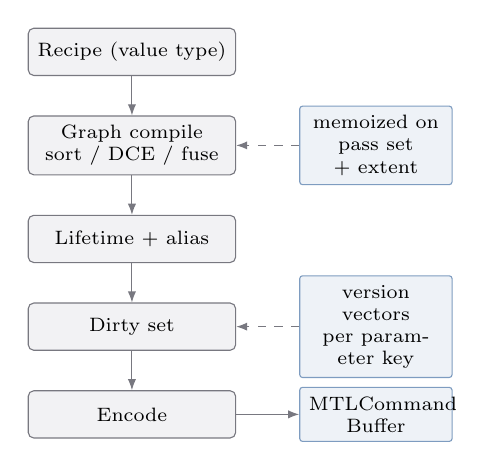
\begin{tikzpicture}[
  font=\scriptsize,
  box/.style={draw=emLine, rounded corners=2pt, minimum height=6mm, text width=24mm, align=center, fill=emGray},
  res/.style={draw=emBlue!60, fill=emBlue!8, rounded corners=1pt, minimum height=5mm, text width=17mm, align=center},
  ar/.style={-{Latex[length=1.4mm]}, draw=emLine}
]
\node[box] (r) at (0,0) {Recipe (value type)};
\node[box, below=5mm of r] (c) {Graph compile\\\scriptsize sort / DCE / fuse};
\node[box, below=5mm of c] (a) {Lifetime + alias};
\node[box, below=5mm of a] (d) {Dirty set};
\node[box, below=5mm of d] (e) {Encode};

\node[res, right=8mm of c] (m1) {memoized on\\pass set + extent};
\node[res, right=8mm of d] (m2) {version vectors\\per parameter key};
\node[res, right=8mm of e] (m3) {MTLCommand\\Buffer};

\foreach \x/\y in {r/c, c/a, a/d, d/e} \draw[ar] (\x) -- (\y);
\draw[ar, dashed] (m1) -- (c);
\draw[ar, dashed] (m2) -- (d);
\draw[ar] (e) -- (m3);
\end{tikzpicture}
\caption{Render graph execution flow. Compilation is memoized; steady-state slider dragging touches only the dirty set and the encode step.}
\label{fig:graphflow}
\end{figure}

\subsection{Testability}

The graph is a pure data structure until \texttt{encode} is called, which makes
several important properties unit-testable without a GPU:

\begin{itemize}
\item \textbf{Topology.} Given a recipe, assert the compiled pass list. This
catches accidental reordering, which is the highest-severity class of imaging
regression.
\item \textbf{Dead pass elimination.} Assert that disabling halation removes
five passes.
\item \textbf{Aliasing correctness.} Assert that no two resources with
overlapping live intervals share an allocation offset. This is checked
exhaustively by a property-based test over randomly generated graphs.
\item \textbf{Dirty propagation.} Assert the re-run set for each parameter key
matches Table~\ref{tab:dirtycost}. This table is generated \emph{from} the test,
not written by hand, so it cannot drift.
\end{itemize}

\section{Application Architecture}
\label{sec:apparch}

\subsection{Domain Model}

The domain is built on value types so that state is trivially snapshot-able,
diffable, and thread-safe.

\begin{lstlisting}[language=Swift, caption={Core domain types.}, label={lst:domain}]
/// A complete, self-contained description of how to develop one image.
struct Recipe: Codable, Hashable, Sendable {
    var negativeStock : StockRef
    var printStock    : PrintStockRef
    var chemistry     : ChemistryRef

    var capture   : CaptureStage      // exposure comp, WB, rating
    var develop   : DevelopStage      // push/pull, time, temp, agitation
    var interlayer: InterlayerStage
    var printing  : PrintStage        // printer lights, density, sat.
    var grain     : GrainStage
    var halation  : HalationStage
    var optical   : OpticalStage
    var aging     : AgingStage
    var output    : OutputStage       // color space, surround, crop

    var format    : FilmFormat        // drives all physical scaling
    var seed      : UInt32            // grain / dust / leak realization
}

/// Stable identity for every scalar the pipeline consumes.
enum ParameterKey: String, CaseIterable, Codable, Sendable {
    case exposureCompensation, filmSpeed, whiteBalanceTemp, whiteBalanceTint
    case pushPull, developmentTime, developmentTemp, agitation
    case couplerActivity
    case printerLightR, printerLightG, printerLightB, printDensity
    case saturationDensity, highlightRolloff, shadowLift
    case neutralAxisWarm, neutralAxisTint, silverRetention
    case grainAmount, grainSize, grainSeed
    case halationThreshold, halationRadius, halationIntensity, halationBias
    case diffusionAmount, vignetteAmount, chromaticAberration
    case distortionK1, distortionK2
    case dustDensity, scratchDensity, edgeFog, lightLeak, expiredAge
    // ...
}
\end{lstlisting}

\texttt{Recipe} is \texttt{Codable}, which gives sidecar export
(FR-17) and database persistence for free, and \texttt{Hashable}, which gives
cheap change detection. Every field has a documented default, and a
\texttt{Recipe} constructed with defaults plus a stock reference is a valid,
renderable state --- there is no partially-initialized recipe.

\subsection{Parameter Resolution}

A rendered image's parameters are the result of layering four sources, resolved
in order:

\begin{enumerate}
\item Stock profile defaults (from the profile bundle).
\item Chemistry profile modulation (Section~\ref{sec:development}).
\item Recipe values (the user's edit).
\item Transient overrides (preview quality reductions, gesture state).
\end{enumerate}

Resolution produces a \texttt{ResolvedParameters} struct --- a flat, contiguous
value with no optionals --- which is what the render graph consumes. The
separation matters: the UI edits a sparse \texttt{Recipe} where "unset" is
meaningful (so that changing stock changes the defaults for untouched
parameters), while the renderer consumes a dense resolved value where everything
has a number.

\subsection{Edit History}

History is implemented as a list of \texttt{Recipe} snapshots rather than a
command stack. A \texttt{Recipe} is a few hundred bytes; 200 snapshots is under
100\,KB, which is cheaper than the bookkeeping a command pattern requires and is
immune to the classic inverse-command bug where undo does not exactly restore
prior state.

Snapshots are \emph{coalesced} by a policy that merges consecutive edits to the
same parameter key within a 700\,ms window, so that a slider drag produces one
undo step rather than four hundred. The coalescing rule is expressed on the key,
not on time alone --- switching parameters always commits a step, so the user's
mental model of undo matches the visual grouping of controls.

\begin{lstlisting}[language=Swift, caption={History with key-aware coalescing.}]
struct History {
    private(set) var stack: [Entry] = []
    private(set) var cursor: Int = -1
    private var lastKey: ParameterKey?
    private var lastAt: ContinuousClock.Instant?

    mutating func record(_ r: Recipe, key: ParameterKey?, now: ContinuousClock.Instant) {
        let coalesce = key != nil && key == lastKey
            && lastAt.map { now - $0 < .milliseconds(700) } ?? false
        if coalesce, cursor >= 0 {
            stack[cursor].recipe = r          // replace in place
        } else {
            stack.removeSubrange((cursor + 1)...)   // drop redo branch
            stack.append(Entry(recipe: r, key: key, at: now))
            cursor = stack.count - 1
            if stack.count > 200 { stack.removeFirst(); cursor -= 1 }
        }
        lastKey = key; lastAt = now
    }
}
\end{lstlisting}

\subsection{The Render Actor State Machine}

The coalescing behavior described in Section~\ref{sec:arch} is specified here
precisely, because it is the difference between a responsive and a laggy editor
and it is easy to get subtly wrong.

\begin{lstlisting}[language=Swift, caption={Render actor with single-slot coalescing.}, label={lst:renderactor}]
actor RenderCoordinator {
    private var inFlight: Bool = false
    private var pending: RenderRequest?
    private let graph: RenderGraph

    /// Called from the main actor on every parameter change. Never blocks.
    func submit(_ request: RenderRequest) {
        pending = request                 // overwrite: only latest matters
        guard !inFlight else { return }   // completion handler will pick it up
        drain()
    }

    private func drain() {
        guard let req = pending else { inFlight = false; return }
        pending = nil
        inFlight = true

        let cb = queue.makeCommandBuffer()!
        do { try graph.encode(req, into: cb) }
        catch { inFlight = false; report(error); return }

        cb.addCompletedHandler { [weak self] _ in
            Task { await self?.drain() }   // pick up whatever arrived meanwhile
        }
        cb.commit()
    }
}
\end{lstlisting}

Three properties follow and are asserted by test:

\begin{itemize}
\item At most one command buffer is in flight, bounding memory and latency.
\item Intermediate parameter values during a fast drag are dropped rather than
queued, so latency does not accumulate.
\item The final value of a drag is always rendered, because the last
\texttt{submit} sets \texttt{pending} and the completion handler will drain it.
The naive "skip if busy" implementation loses the final value and leaves a stale
image, which is a defect that only appears when the user flicks a slider and
lets go --- and which is therefore routinely shipped.
\end{itemize}

\subsection{Capture Subsystem}

Capture uses \texttt{AVCaptureSession} with a \texttt{AVCapturePhotoOutput}
configured for Bayer or ProRAW output depending on device capability.

\begin{lstlisting}[language=Swift, caption={ProRAW capture configuration.}]
func makeSettings(output: AVCapturePhotoOutput) -> AVCapturePhotoSettings {
    // Prefer Apple ProRAW (linear DNG with Apple's computational stack applied
    // to the mosaic) over plain Bayer RAW: it carries the multi-frame
    // noise reduction we do not wish to reimplement, while remaining linear.
    if output.isAppleProRAWSupported {
        output.isAppleProRAWEnabled = true
    }
    let fmt = output.availableRawPhotoPixelFormatTypes.first {
        AVCapturePhotoOutput.isAppleProRAWPixelFormat($0)
    } ?? output.availableRawPhotoPixelFormatTypes.first!

    let s = AVCapturePhotoSettings(rawPixelFormatType: fmt,
                                   processedFormat: [AVVideoCodecKey: AVVideoCodecType.hevc])
    s.photoQualityPrioritization = .quality
    s.isHighResolutionPhotoEnabled = true
    s.embeddedThumbnailPhotoFormat = [AVVideoCodecKey: AVVideoCodecType.jpeg]
    return s
}
\end{lstlisting}

Manual controls are exposed through \texttt{AVCaptureDevice} lock:
\texttt{setExposureModeCustom} for shutter and ISO,
\texttt{setFocusModeLocked} for manual focus with a lens-position slider, and
\texttt{setWhiteBalanceModeLocked} with device gains computed from a temperature
and tint pair. The camera preview shows a live approximation of the selected
recipe (Section~\ref{sec:liveview}), not the raw sensor image, since seeing the
intended result while composing is the primary reason a photographer would use
this application's camera rather than the system one.

\subsection{Live Preview Approximation}
\label{sec:liveview}

The full pipeline at video rates on the preview stream is achievable but is not
a good use of thermal budget while composing. The live view therefore runs a
reduced graph:

\begin{itemize}
\item The pointwise chain runs at full fidelity, via the same baked 3D LUT
(Section~\ref{sec:lutbake}) applied to the preview stream. This is a single
texture fetch and is what determines the color, which is what the user is
judging.
\item Halation runs with a two-level pyramid instead of four.
\item Grain and aging are disabled, with a small badge indicating so.
\item Optical simulation runs vignetting only.
\end{itemize}

Measured cost is 2.8\,ms per frame at $1920\times1440$ preview resolution on an
A17 Pro, comfortably inside the 33\,ms frame budget with substantial thermal
headroom.

\subsection{Import Pipeline}

Imported files traverse: security-scoped URL resolution; format probe;
\texttt{CIRAWFilter} construction and metadata extraction; copy into the
application's managed store (or, for Photos assets, retention of a
\texttt{PHAsset} local identifier plus a cached decode); thumbnail generation at
three sizes; and a database insert. The entire operation runs on the I/O queue
and reports progress; a batch import of 200 DNGs completes in approximately
40\,s, dominated by thumbnail decode.

Imported files whose color characterization cannot be determined (an unusual
TIFF, a DNG from an unknown camera) are flagged and given a conservative
assumed-sRGB interpretation, with a visible advisory. Silently guessing is worse
than saying so.

\subsection{Error Handling Policy}

Errors are classified and handled by class rather than individually:

\begin{table}[htbp]
\caption{Error Classification}
\label{tab:errors}
\begin{center}
\renewcommand{\arraystretch}{1.15}
\begin{tabularx}{\columnwidth}{@{}l>{\raggedright\arraybackslash}X@{}}
\toprule
\textbf{Class} & \textbf{Policy} \\
\midrule
Programmer error & Trap in debug, log and degrade in release. Graph cycles, missing pipeline states, impossible parameter combinations. \\
Resource exhaustion & Reduce quality tier and retry once; then surface. Applies to heap allocation and export tiling. \\
Device loss / GPU fault & Recreate device objects, rebuild caches, re-render. Report once per session. \\
User data error & Surface with a specific, actionable message. Unsupported file, corrupt DNG, missing permission. \\
Transient & Retry with backoff, silent. Photos library access contention, file coordination. \\
\bottomrule
\end{tabularx}
\end{center}
\end{table}

\section{User Interface Design}
\label{sec:ui}

\subsection{Interaction Principles}

Four principles govern the interface, in priority order when they conflict.

\begin{enumerate}
\item \textbf{The image is the interface.} Controls overlay or dock; they never
crop the image below 55\% of the screen area. Any control that requires the
image to shrink is a modal sheet, not a permanent chrome element.
\item \textbf{One vocabulary.} The names in Table~\ref{tab:controlmap} appear
identically in the UI, in the tooltip, in the exported metadata, and in this
document. There is no simplified alias.
\item \textbf{Progressive disclosure without a beginner mode.} Every panel has
a primary row of two to four controls and a disclosure for the remainder. The
beginner and the professional use the same controls; the beginner sees fewer at
once.
\item \textbf{Every control teaches.} Long-pressing any control presents a
one-paragraph explanation of the physical process it corresponds to, with a
diagram where useful. This is the mechanism by which the product's central claim
--- that development is more truthful than filtering --- becomes something the
user experiences rather than reads in marketing copy.
\end{enumerate}

\subsection{Navigation Structure}

Three root workspaces in a tab structure: \textbf{Capture}, \textbf{Develop},
\textbf{Library}. Develop is reachable only with an active asset; selecting an
asset in Library or completing a capture pushes into it. This is a shallow
hierarchy by design --- the deepest navigation path in the application is three
levels (Library $\to$ Develop $\to$ Stage detail).

\begin{figure*}[htbp]
\centering
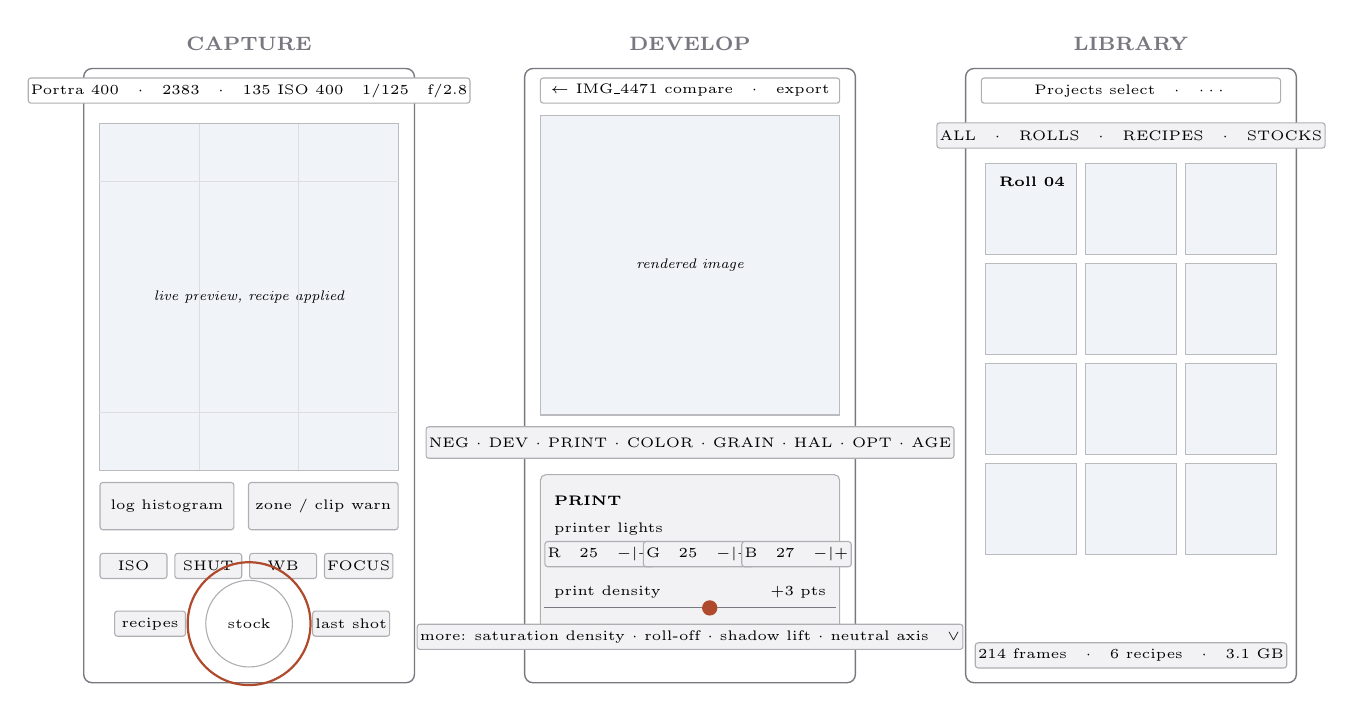
\begin{tikzpicture}[
  font=\tiny,
  phone/.style={draw=emLine, line width=0.5pt, rounded corners=3pt, minimum width=42mm, minimum height=78mm},
  ctl/.style={draw=emLine!60, fill=emGray, rounded corners=1pt, minimum height=3.2mm, inner sep=1pt, align=center},
  img/.style={draw=emLine!50, fill=emBlue!7, minimum width=38mm},
  lbl/.style={font=\tiny\bfseries},
  wfcap/.style={font=\scriptsize\bfseries, text=emLine}
]

%============ CAPTURE ============
\begin{scope}[shift={(0,0)}]
  \node[phone] (p1) at (0,0) {};
  \node[wfcap, above=1mm of p1.north] {CAPTURE};
  % status bar
  \node[ctl, minimum width=38mm, fill=white] at (0,3.62) {\tiny Portra 400 \; $\cdot$ \; 2383 \; $\cdot$ \; 135 \hfill ISO 400 \; 1/125 \; f/2.8};
  % viewfinder
  \node[img, minimum height=44mm] (vf) at (0,1.0) {};
  \node at (0,1.0) {\itshape live preview, recipe applied};
  % grid overlay hint
  \draw[emLine!25] (-1.9,-0.47) -- (1.9,-0.47);
  \draw[emLine!25] (-1.9,2.47) -- (1.9,2.47);
  \draw[emLine!25] (-0.63,-1.2) -- (-0.63,3.2);
  \draw[emLine!25] (0.63,-1.2) -- (0.63,3.2);
  % histogram
  \node[ctl, minimum width=17mm, minimum height=6mm, anchor=north west] at (-1.9,-1.35) {\tiny log histogram};
  \node[ctl, minimum width=19mm, minimum height=6mm, anchor=north east] at (1.9,-1.35) {\tiny zone / clip warn};
  % manual control strip
  \node[ctl, minimum width=8.5mm, anchor=north west] at (-1.9,-2.25) {ISO};
  \node[ctl, minimum width=8.5mm, anchor=north west] at (-0.95,-2.25) {SHUT};
  \node[ctl, minimum width=8.5mm, anchor=north west] at (0.0,-2.25) {WB};
  \node[ctl, minimum width=8.5mm, anchor=north west] at (0.95,-2.25) {FOCUS};
  % dial
  \draw[emLine!60] (0,-3.15) circle (0.55);
  \node at (0,-3.15) {\tiny stock};
  \node[ctl, minimum width=9mm, anchor=east] at (-0.8,-3.15) {recipes};
  \node[ctl, minimum width=9mm, anchor=west] at (0.8,-3.15) {last shot};
  % shutter
  \draw[emAcc, line width=0.8pt] (0,-3.15) circle (0.78);
\end{scope}

%============ DEVELOP ============
\begin{scope}[shift={(5.6,0)}]
  \node[phone] (p2) at (0,0) {};
  \node[wfcap, above=1mm of p2.north] {DEVELOP};
  \node[ctl, minimum width=38mm, fill=white] at (0,3.62) {\tiny $\leftarrow$ \hfill IMG\_4471 \hfill compare \; $\cdot$ \; export};
  \node[img, minimum height=38mm] (im) at (0,1.4) {};
  \node at (0,1.4) {\itshape rendered image};
  % stage rail
  \node[ctl, minimum width=38mm, minimum height=4mm] at (0,-0.85)
    {\tiny NEG $\cdot$ DEV $\cdot$ PRINT $\cdot$ COLOR $\cdot$ GRAIN $\cdot$ HAL $\cdot$ OPT $\cdot$ AGE};
  % active panel
  \node[draw=emLine!60, fill=emGray, rounded corners=2pt, minimum width=38mm, minimum height=22mm, anchor=north] (panel) at (0,-1.25) {};
  \node[lbl, anchor=north west] at (-1.85,-1.4) {PRINT};
  % printer lights
  \node[anchor=north west, align=left] at (-1.85,-1.75)
    {\tiny printer lights};
  \node[ctl, minimum width=11mm, anchor=north west] at (-1.85,-2.1) {R \; 25 \; $-|+$};
  \node[ctl, minimum width=11mm, anchor=north west] at (-0.6,-2.1) {G \; 25 \; $-|+$};
  \node[ctl, minimum width=11mm, anchor=north west] at (0.65,-2.1) {B \; 27 \; $-|+$};
  % density slider
  \node[anchor=north west] at (-1.85,-2.55) {\tiny print density};
  \draw[emLine] (-1.85,-2.95) -- (1.85,-2.95);
  \draw[emAcc, fill=emAcc] (0.25,-2.95) circle (0.09);
  \node[anchor=north east] at (1.85,-2.55) {\tiny $+3$ pts};
  % disclosure
  \node[ctl, minimum width=38mm, anchor=north] at (0,-3.15) {\tiny more: saturation density $\cdot$ roll-off $\cdot$ shadow lift $\cdot$ neutral axis \; $\vee$};
\end{scope}

%============ LIBRARY ============
\begin{scope}[shift={(11.2,0)}]
  \node[phone] (p3) at (0,0) {};
  \node[wfcap, above=1mm of p3.north] {LIBRARY};
  \node[ctl, minimum width=38mm, fill=white] at (0,3.62) {\tiny Projects \hfill select \; $\cdot$ \; $\cdots$};
  % segmented
  \node[ctl, minimum width=38mm] at (0,3.05) {\tiny ALL \; $\cdot$ \; ROLLS \; $\cdot$ \; RECIPES \; $\cdot$ \; STOCKS};
  % grid
  \foreach \r in {0,1,2,3} {
    \foreach \c in {0,1,2} {
      \node[img, minimum width=11.5mm, minimum height=11.5mm, anchor=north west]
        at (-1.85+\c*1.27, 2.7-\r*1.27) {};
    }
  }
  \node[anchor=north west] at (-1.8,2.65) {\tiny \textbf{Roll 04}};
  % footer
  \node[ctl, minimum width=38mm, anchor=south] at (0,-3.72) {\tiny 214 frames \; $\cdot$ \; 6 recipes \; $\cdot$ \; 3.1 GB};
\end{scope}

\end{tikzpicture}
\caption{Primary workspace wireframes. Capture keeps the manual control strip and the stock dial within thumb reach of the shutter. Develop devotes the upper 55\% to the image with a horizontal stage rail selecting the active panel below. Library is grid-first with roll grouping, since users organize by shooting session.}
\label{fig:wireframes}
\end{figure*}

\subsection{The Develop Workspace}

The stage rail in Figure~\ref{fig:wireframes} is the structural expression of
the pipeline. Selecting a stage swaps the panel below without changing the image
area, so comparisons across stages do not shift the frame.

Each panel follows an identical layout contract:

\begin{itemize}
\item A title matching the pipeline stage name in Figure~\ref{fig:pipeline}.
\item Two to four \emph{primary} controls, always visible.
\item A disclosure row listing the secondary controls by name, so their
existence is discoverable without being present.
\item A reset affordance scoped to the stage.
\item A bypass toggle, which disables the stage entirely (and, through dead
pass elimination in Section~\ref{sec:rendergraph}, removes its cost).
\end{itemize}

\begin{table}[htbp]
\caption{Panel Contents by Stage}
\label{tab:panels}
\begin{center}
\renewcommand{\arraystretch}{1.15}
\begin{tabularx}{\columnwidth}{@{}l>{\raggedright\arraybackslash}X@{}}
\toprule
\textbf{Panel} & \textbf{Primary / secondary} \\
\midrule
NEG & Stock, film speed rating, exposure comp. / format, layer balance readout, curve inspector \\
DEV & Push/pull, development time / temperature, agitation, chemistry, CI readout \\
PRINT & Printer lights R/G/B, print density / print stock, silver retention \\
COLOR & Saturation density, highlight roll-off / shadow lift, neutral axis warm, neutral axis tint \\
GRAIN & Amount, size / seed, clustering, chroma correlation \\
HAL & Intensity, threshold / radius, color bias, ring weight \\
OPT & Diffusion, vignetting / chromatic aberration, distortion, bloom, defocus \\
AGE & Expired age, dust / scratches, edge fog, light leak, streaking \\
\bottomrule
\end{tabularx}
\end{center}
\end{table}

\subsection{Control Idioms}

Three control types cover the entire parameter surface.

\paragraph{The stepper-slider} Used for all continuous parameters. A horizontal
track with a draggable thumb, a numeric readout in the parameter's physical unit,
and a detent at the physically neutral value. Dragging with one finger is coarse;
a second finger down engages a $5\times$ fine mode without lifting. Double-tap
resets to the stage default.

\paragraph{The printer-point stepper} Used only for printer lights. Integer
increment and decrement buttons flanking a value, with a hold-to-repeat. It is
deliberately \emph{not} a slider, because printer points are integers and
because the tactile discreteness reinforces the unit
(Section~\ref{sec:printerlights}).

\paragraph{The stock dial} A circular selector for negative and print stock,
showing a live thumbnail of the current image under each candidate as it passes
under the selection indicator. Rendering eight thumbnails at $128^2$ costs
approximately 1.2\,ms total, so the previews are live rather than cached ---
which is the single most persuasive interaction in the product, because the user
sees the stock's actual effect on their own image rather than on a sample.

\subsection{Comparison Modes}

FR-19 requires before/after. Three modes are provided:

\begin{itemize}
\item \textbf{Toggle.} Press and hold anywhere on the image to show the
unprocessed scene-referred image with only the output transform applied.
\item \textbf{Split.} A draggable vertical divider. The two sides render from
the same graph with different recipes, sharing all resources whose parameters
are unchanged --- so a split view of a printer-light change costs
$1.9\times$, not $2\times$, and a split of a grain change costs $1.2\times$.
\item \textbf{Pin to stage.} Compare the current state against the pipeline
output at any earlier stage. This is the pipeline inspector of FR-20 expressed
as a comparison rather than as a separate screen, and it is how a user comes to
understand what each stage contributes.
\end{itemize}

\subsection{The Pipeline Inspector}

A full-screen modal presenting the pipeline as the diagram of
Figure~\ref{fig:pipeline}, with a live thumbnail rendered at each node showing
the image state at that point. Tapping a node jumps to its panel; long-pressing
shows the governing equation and the current parameter values.

This screen is, deliberately, the most technically explicit surface in the
product. It is not the default view and most users will visit it rarely. Its
purpose is to make the claim in Section~\ref{sec:intro-thesis} inspectable: a
user who doubts that anything physical is happening can look.

\begin{figure}[htbp]
\centering
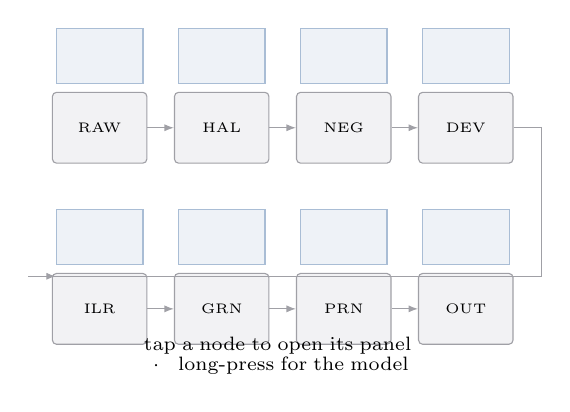
\begin{tikzpicture}[
  font=\tiny,
  nd/.style={draw=emLine!70, fill=emGray, rounded corners=1.5pt, minimum width=12mm, minimum height=9mm, align=center},
  th/.style={draw=emBlue!40, fill=emBlue!8, minimum width=11mm, minimum height=7mm},
  ar/.style={-{Latex[length=1.2mm]}, draw=emLine!70}
]
\foreach \i/\n [count=\j from 0] in {0/RAW, 1/HAL, 2/NEG, 3/DEV} {
  \node[th] (t\i) at (\j*1.55, 0.9) {};
  \node[nd, below=1mm of t\i] (n\i) {\n};
}
\foreach \i/\n [count=\j from 0] in {4/ILR, 5/GRN, 6/PRN, 7/OUT} {
  \node[th] (t\i) at (\j*1.55, -1.4) {};
  \node[nd, below=1mm of t\i] (n\i) {\n};
}
\foreach \a/\b in {n0/n1, n1/n2, n2/n3} \draw[ar] (\a) -- (\b);
\foreach \a/\b in {n4/n5, n5/n6, n6/n7} \draw[ar] (\a) -- (\b);
\draw[ar] (n3.east) -- ++(0.35,0) |- ($(t4.west)+(-0.35,-0.5)$) -- ++(0.35,0);
\node[anchor=north, align=center, text width=52mm] at (2.3,-2.55)
  {\scriptsize tap a node to open its panel \; $\cdot$ \; long-press for the model};
\end{tikzpicture}
\caption{Pipeline inspector layout. Each node shows the live image state at that point in the chain, rendered from the same graph with an early termination.}
\label{fig:inspector}
\end{figure}

\subsection{Gestures}

\begin{table}[htbp]
\caption{Gesture Map}
\label{tab:gestures}
\begin{center}
\renewcommand{\arraystretch}{1.15}
\begin{tabularx}{\columnwidth}{@{}l>{\raggedright\arraybackslash}X@{}}
\toprule
\textbf{Gesture} & \textbf{Action} \\
\midrule
Pinch & Zoom, 1$\times$ to 400\%. Triggers ROI rendering above 100\%. \\
Two-finger pan & Pan when zoomed. \\
Press and hold on image & Show original (toggle compare). \\
Double-tap image & Zoom to 100\% at tap point, or back to fit. \\
Horizontal swipe on stage rail & Change active panel. \\
Horizontal swipe on image & Previous/next asset (only when at fit zoom). \\
Two-finger drag on any slider & Fine adjustment, $5\times$ resolution. \\
Three-finger swipe left/right & Undo / redo (system convention). \\
Long-press control label & Explanation sheet. \\
\bottomrule
\end{tabularx}
\end{center}
\end{table}

Note the conflict resolution between horizontal image swipe (asset change) and
pan: asset swiping is enabled only at fit zoom, where panning is meaningless.
This is checked in the gesture recognizer's \texttt{shouldBegin}, not by
disabling recognizers, so the transition is seamless as the user zooms out.

\subsection{Visual Design}

The visual language is quiet, achromatic, and deferential to the image. The
chrome is a single neutral gray at two elevations, with one accent color used
exclusively for modified-from-default state. This is not minimalism for its own
sake: any chroma in the surrounding UI biases the perception of the image being
graded, which is why professional grading suites are painted neutral gray. The
same reasoning that governs a color suite governs this interface, and it is
stated in the design system documentation so that it survives future
redesigns.

Explicitly excluded: leather textures, film-canister iconography, simulated
light leaks in the chrome, faux-analog typography, sprocket-hole borders, and
any skeuomorphic camera imagery. The application is a laboratory instrument, and
laboratory instruments do not cosplay.

\subsection{Dark and Light Appearance}

Both are supported. Dark is the default, because a dark surround improves the
perception of highlight roll-off and because the application is most often used
in editing rather than reference-viewing contexts. The image area's immediate
surround is held at a fixed 18\% neutral in \emph{both} appearances, since a
pure-black or pure-white surround measurably shifts perceived contrast; only the
outer chrome changes with appearance.

\subsection{Accessibility}

NFR-11 is met by: VoiceOver labels for every control stating name, value, and
unit ("printer light red, 25 points"); custom rotors for stage navigation and
for parameter adjustment; Dynamic Type support to XXL in all text, with panels
reflowing to a vertical layout at large sizes; Reduce Motion honored by
replacing panel transitions with cross-fades; and a minimum 44$\times$44 point
touch target for every interactive element including the printer-point steppers.

Color is never the sole carrier of information. The modified-from-default
indicator is an accent color \emph{and} a shape change on the slider detent.
Clipping warnings use a diagonal hatch pattern rather than a color overlay.

\section{Persistence and Data Model}
\label{sec:schema}

\subsection{Storage Technology}

SQLite via GRDB is used rather than Core Data or SwiftData. The reasons are
specific and were weighed against the convenience cost:

\begin{itemize}
\item The schema is relational and query-heavy (library filtering, recipe
usage counts, cache eviction by LRU), which is SQL's home ground.
\item Migrations must be explicit and testable. The imaging model will evolve
across releases and a user's edit history must survive it; an inferred
migration is not acceptable for data the user cannot recreate.
\item Write patterns include high-frequency small writes (edit autosave) that
benefit from WAL mode and explicit transaction control.
\item The domain layer is already plain Swift values
(Section~\ref{sec:apparch}); an object graph framework would push framework
types into the domain, violating the layering of Table~\ref{tab:layers}.
\end{itemize}

The database is opened in WAL mode \cite{sqlitewal} with
\texttt{synchronous = NORMAL},
\texttt{foreign\_keys = ON}, and a 20\,MB page cache.

\subsection{Entity Relationship Overview}

\begin{figure}[htbp]
\centering
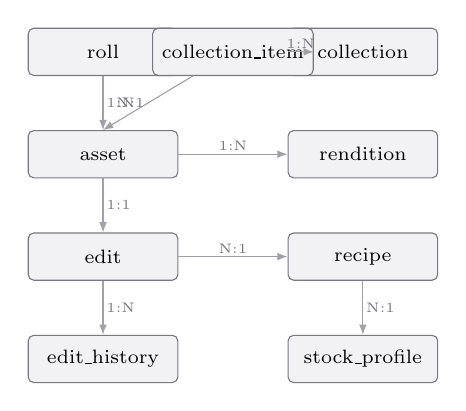
\begin{tikzpicture}[
  font=\scriptsize,
  ent/.style={draw=emLine, fill=emGray, rounded corners=2pt, minimum width=19mm, minimum height=6mm, align=center},
  rel/.style={draw=emLine!70, -{Latex[length=1.3mm]}},
  card/.style={font=\tiny, text=emLine, inner sep=1pt}
]
\node[ent] (roll)   at (0,3.2)   {roll};
\node[ent] (asset)  at (0,1.9)   {asset};
\node[ent] (edit)   at (0,0.6)   {edit};
\node[ent] (hist)   at (0,-0.7)  {edit\_history};
\node[ent] (rend)   at (3.3,1.9) {rendition};
\node[ent] (recipe) at (3.3,0.6) {recipe};
\node[ent] (stock)  at (3.3,-0.7){stock\_profile};
\node[ent] (coll)   at (3.3,3.2) {collection};
\node[ent] (memb)   at (1.65,3.2){collection\_item};

\draw[rel] (roll)  -- (asset)  node[card, midway, right] {1:N};
\draw[rel] (asset) -- (edit)   node[card, midway, right] {1:1};
\draw[rel] (edit)  -- (hist)   node[card, midway, right] {1:N};
\draw[rel] (asset) -- (rend)   node[card, midway, above] {1:N};
\draw[rel] (edit)  -- (recipe) node[card, midway, above] {N:1};
\draw[rel] (recipe)-- (stock)  node[card, midway, right] {N:1};
\draw[rel] (coll)  -- (memb)   node[card, midway, above] {1:N};
\draw[rel] (memb)  -- (asset.north) node[card, midway, left] {N:1};
\end{tikzpicture}
\caption{Entity relationships. \texttt{edit} carries the live recipe for an asset; \texttt{recipe} stores named, reusable parameter sets; \texttt{rendition} caches derived images keyed by content hash.}
\label{fig:erd}
\end{figure}

\subsection{Schema}

The complete DDL is given in Appendix~\ref{app:ddl}. The essential tables and
their design rationale follow.

\begin{lstlisting}[language=SQL, caption={Asset and roll tables.}, label={lst:ddl-asset}]
CREATE TABLE roll (
    id              TEXT PRIMARY KEY,          -- UUID
    name            TEXT NOT NULL,
    created_at      REAL NOT NULL,             -- Unix epoch, UTC
    -- A roll may carry a default recipe applied to new captures,
    -- which is how "shoot a roll of Portra" works as a workflow.
    default_recipe_id TEXT REFERENCES recipe(id) ON DELETE SET NULL,
    notes           TEXT
) STRICT;

CREATE TABLE asset (
    id              TEXT PRIMARY KEY,
    roll_id         TEXT REFERENCES roll(id) ON DELETE SET NULL,
    -- Exactly one of these two is non-null.
    file_relpath    TEXT,        -- managed store, relative to container
    ph_local_id     TEXT,        -- Photos library asset identifier
    content_hash    TEXT NOT NULL,             -- SHA-256 of source bytes
    original_uti    TEXT NOT NULL,
    pixel_width     INTEGER NOT NULL,
    pixel_height    INTEGER NOT NULL,
    captured_at     REAL,
    imported_at     REAL NOT NULL,
    -- Denormalized capture metadata for fast library filtering; the
    -- authoritative copy remains in the file.
    camera_model    TEXT,
    lens_model      TEXT,
    iso             INTEGER,
    exposure_time   REAL,
    f_number        REAL,
    focal_length    REAL,
    gps_lat         REAL,
    gps_lon         REAL,
    is_favorite     INTEGER NOT NULL DEFAULT 0,
    deleted_at      REAL,                      -- soft delete, 30-day purge
    CHECK ((file_relpath IS NULL) <> (ph_local_id IS NULL))
) STRICT;

CREATE INDEX idx_asset_roll     ON asset(roll_id, captured_at DESC);
CREATE INDEX idx_asset_captured ON asset(captured_at DESC) WHERE deleted_at IS NULL;
CREATE UNIQUE INDEX idx_asset_hash ON asset(content_hash) WHERE deleted_at IS NULL;
\end{lstlisting}

Three decisions in Listing~\ref{lst:ddl-asset} deserve comment. The
\texttt{CHECK} constraint enforcing exactly one storage location prevents the
ambiguous state where an asset is both managed and Photos-backed, which would
otherwise produce duplicate-detection bugs. The unique index on
\texttt{content\_hash} is partial, so soft-deleted assets do not block
re-import of the same file. And capture metadata is denormalized deliberately:
library filtering by camera or focal length must not require opening files.

\begin{lstlisting}[language=SQL, caption={Edit and history tables.}, label={lst:ddl-edit}]
CREATE TABLE edit (
    asset_id        TEXT PRIMARY KEY REFERENCES asset(id) ON DELETE CASCADE,
    -- The live recipe as canonical JSON. Stored as text rather than
    -- decomposed columns because the parameter set is versioned and
    -- evolves; a column-per-parameter schema would migrate on every
    -- imaging change.
    recipe_json     TEXT NOT NULL,
    recipe_version  INTEGER NOT NULL,          -- schema version of the JSON
    -- Hash of recipe_json; the rendition cache key.
    recipe_hash     TEXT NOT NULL,
    source_recipe_id TEXT REFERENCES recipe(id) ON DELETE SET NULL,
    updated_at      REAL NOT NULL
) STRICT;

CREATE TABLE edit_history (
    id              INTEGER PRIMARY KEY AUTOINCREMENT,
    asset_id        TEXT NOT NULL REFERENCES asset(id) ON DELETE CASCADE,
    seq             INTEGER NOT NULL,          -- position in the stack
    recipe_json     TEXT NOT NULL,
    changed_key     TEXT,                      -- ParameterKey raw value
    created_at      REAL NOT NULL
) STRICT;

CREATE UNIQUE INDEX idx_hist_asset_seq ON edit_history(asset_id, seq);
\end{lstlisting}

Storing the recipe as canonical JSON rather than as a wide table is the most
consequential schema decision in the application. The alternative --- a column
per parameter --- would require a migration on every imaging change, which will
happen many times. The JSON approach requires an in-application version field
and a migration chain for the JSON itself, which is code rather than schema, is
unit-testable, and can be applied lazily on read. The cost is that SQL cannot
query inside a recipe efficiently; this is mitigated by extracting the two
fields that actually need querying (\texttt{recipe\_hash} and
\texttt{source\_recipe\_id}) into real columns.

\begin{lstlisting}[language=SQL, caption={Recipe and stock profile tables.}, label={lst:ddl-recipe}]
CREATE TABLE recipe (
    id              TEXT PRIMARY KEY,
    name            TEXT NOT NULL,
    recipe_json     TEXT NOT NULL,
    recipe_version  INTEGER NOT NULL,
    is_builtin      INTEGER NOT NULL DEFAULT 0,
    -- Thumbnail rendered from a fixed reference image, so the recipe
    -- browser shows what each recipe does without an active asset.
    swatch_blob     BLOB,
    use_count       INTEGER NOT NULL DEFAULT 0,
    last_used_at    REAL,
    created_at      REAL NOT NULL,
    sort_order      INTEGER NOT NULL DEFAULT 0
) STRICT;

CREATE TABLE stock_profile (
    id              TEXT PRIMARY KEY,          -- e.g. "neg.portra400"
    kind            TEXT NOT NULL,             -- 'negative'|'print'|'mono'
    display_name    TEXT NOT NULL,
    -- Versioned so a profile correction can ship without silently
    -- changing the appearance of the user's existing edits; the edit
    -- records the profile version it was authored against.
    profile_version INTEGER NOT NULL,
    params_json     TEXT NOT NULL,             -- theta, A, C, grain, halation
    is_builtin      INTEGER NOT NULL DEFAULT 1,
    CHECK (kind IN ('negative','print','mono'))
) STRICT;
\end{lstlisting}

The \texttt{profile\_version} column addresses a real hazard. If a shipped
stock profile is later corrected --- and it will be, since profiles are fits to
measurement --- every existing edit made with that stock would silently change
appearance on update. \EM{} instead retains superseded profile versions and
binds each edit to the version it was authored against, offering an explicit
"update to corrected profile" action with a before/after preview. Silently
altering a user's finished images is a violation of the non-destructive promise
in FR-12, even though no file changed.

\begin{lstlisting}[language=SQL, caption={Rendition cache.}, label={lst:ddl-rend}]
CREATE TABLE rendition (
    id              INTEGER PRIMARY KEY AUTOINCREMENT,
    asset_id        TEXT NOT NULL REFERENCES asset(id) ON DELETE CASCADE,
    -- Cache key: (recipe_hash, size class, color space, profile versions)
    cache_key       TEXT NOT NULL,
    size_class      TEXT NOT NULL,   -- 'thumb'|'grid'|'screen'|'full'
    pixel_width     INTEGER NOT NULL,
    pixel_height    INTEGER NOT NULL,
    color_space     TEXT NOT NULL,
    file_relpath    TEXT NOT NULL,
    byte_size       INTEGER NOT NULL,
    created_at      REAL NOT NULL,
    last_access_at  REAL NOT NULL,
    CHECK (size_class IN ('thumb','grid','screen','full'))
) STRICT;

CREATE UNIQUE INDEX idx_rend_key ON rendition(cache_key);
CREATE INDEX idx_rend_lru ON rendition(last_access_at);
\end{lstlisting}

Cache eviction (NFR-12) is a straightforward LRU over
\texttt{idx\_rend\_lru}, with the constraint that \texttt{thumb} and
\texttt{grid} renditions for non-deleted assets are evicted last, since
regenerating them is what makes the library feel slow. Eviction runs on a
background task when total \texttt{byte\_size} exceeds 3.5\,GB, targeting
2.5\,GB.

\subsection{Migration Strategy}

Two independent version dimensions exist and must not be conflated:

\begin{enumerate}
\item \textbf{Schema version} --- the SQL structure, migrated by GRDB's
\texttt{DatabaseMigrator} with one registered, named, immutable migration per
change. Migrations are never edited after release; corrections ship as new
migrations.
\item \textbf{Recipe JSON version} --- the parameter model, migrated in Swift
by a chain of pure functions $f_n: \mathrm{JSON}_n \to \mathrm{JSON}_{n+1}$.
\end{enumerate}

Recipe migration is lazy: a recipe is migrated on read and written back only
when the asset is next edited. This avoids a long blocking migration on update
for users with large libraries, which is a common source of one-star reviews.

The migration chain is tested by a golden-file suite: for each historical
version, a corpus of recipes is stored, migrated forward to current, rendered,
and compared against a stored reference image with a $\Delta E_{00}$
\cite{sharma2005} tolerance.
This is the only mechanism that reliably catches a migration that parses
successfully but changes appearance.

\begin{lstlisting}[language=Swift, caption={Migration registration.}]
var migrator = DatabaseMigrator()
#if DEBUG
migrator.eraseDatabaseOnSchemaChange = true    // development only
#endif

migrator.registerMigration("v1_initial") { db in
    try db.execute(sql: ddlV1)
}
migrator.registerMigration("v2_rendition_lru") { db in
    try db.alter(table: "rendition") { t in
        t.add(column: "last_access_at", .double).notNull().defaults(to: 0)
    }
    try db.create(index: "idx_rend_lru", on: "rendition", columns: ["last_access_at"])
}
migrator.registerMigration("v3_profile_versioning") { db in
    try db.alter(table: "stock_profile") { t in
        t.add(column: "profile_version", .integer).notNull().defaults(to: 1)
    }
}
\end{lstlisting}

\subsection{Sidecar Format}

FR-17 requires an interchangeable recipe file. The format is JSON with a
documented schema:

\begin{lstlisting}[language=Swift, caption={Sidecar structure (illustrative).}]
{
  "emulsion":       { "format": 1, "app": "1.0.0" },
  "recipeVersion":  4,
  "name":           "Portra 400 / 2383, warm",
  "negativeStock":  { "id": "neg.portra400", "version": 3 },
  "printStock":     { "id": "prt.2383",      "version": 2 },
  "chemistry":      { "id": "chem.c41",      "version": 1 },
  "format":         "135",
  "seed":           874112035,
  "parameters": {
    "pushPull":        0.0,
    "printerLightR":  25, "printerLightG": 25, "printerLightB": 27,
    "printDensity":    3,
    "grainAmount":     1.0,
    "halationIntensity": 0.22
  },
  "provenance": {
    "createdAt": "2026-03-14T09:22:41Z",
    "sourceAsset": "5C1B...",
    "note": "matched to lab scan of roll 04 frame 12"
  }
}
\end{lstlisting}

Only parameters that differ from the resolved defaults are written, which keeps
sidecars small and, more importantly, means a sidecar authored against one stock
applies sensibly to another --- the unspecified parameters take the new stock's
defaults rather than the old stock's values. This is the correct semantics for a
"look" and it falls directly out of the sparse-recipe design of
Section~\ref{sec:apparch}.

\section{Performance Engineering}
\label{sec:performance}

\subsection{Budget Derivation}

NFR-01 sets a 16\,ms budget for a preview update. That budget is not all
available to the pipeline: SwiftUI layout and the drawable present consume
approximately 3\,ms, and a safety margin of 2\,ms is reserved to avoid missed
vsync under load. The pipeline budget is therefore \textbf{11\,ms at preview
resolution}.

NFR-02 sets 2.5\,s for a 48\,MP export. At $4032\times3024 = 12.2$\,M pixels
(the ProRAW maximum in the standard mode) or $8064\times6048 = 48.8$\,M pixels
(the high-resolution mode), and with the export path permitted to tile, the
binding constraint is memory bandwidth rather than latency.

\subsection{Bandwidth Analysis}

Bandwidth, not arithmetic, is the limiting resource. The analysis proceeds by
counting full-resolution texture traversals.

Let $N$ be the pixel count and $b$ the bytes per pixel of the working format
(8 for \texttt{rgba16f}). An unfused pass costs $2Nb$ bytes of traffic. On an
A17 Pro, achievable bandwidth for a well-coalesced compute kernel measures
approximately 68\,GB/s in practice against a theoretical peak considerably
higher.

At $N = 48.8$\,M and $b = 8$:

\begin{equation}
\text{traffic per pass} = 2 \times 48.8\times10^6 \times 8 = 781\text{ MB},
\end{equation}

giving 11.5\,ms per unfused full-resolution pass. The naive fourteen-pass
pipeline would therefore require 161\,ms of pure memory traffic --- well within
the 2.5\,s export budget, but $10\times$ over the interactive budget if the
same structure were used for preview.

The fusion strategy of Section~\ref{sec:metal} reduces the full-resolution
traversal count from fourteen to five:

\begin{table}[htbp]
\caption{Full-Resolution Traversals After Fusion}
\label{tab:traversals}
\begin{center}
\renewcommand{\arraystretch}{1.15}
\begin{tabularx}{\columnwidth}{@{}>{\raggedright\arraybackslash}Xcc@{}}
\toprule
\textbf{Fused group} & \textbf{Passes} & \textbf{Traversals} \\
\midrule
Decode + normalize + optics warp + halation source & 4 & 1 \\
Halation pyramid (down/up, geometric) & 8 & 0.33 \\
Halation combine + curve + LUT (tile) & 3 & 1 \\
Interlayer blur $\times 2$ (separable) & 4 & 1.33 \\
Interlayer combine + grain + print (tile) & 4 & 1 \\
Aging + output transform + encode (tile) & 3 & 0.67 \\
\midrule
\textbf{Total} & \textbf{26} & \textbf{5.33} \\
\bottomrule
\end{tabularx}
\end{center}
\end{table}

Five and a third traversals at 11.5\,ms each is 61\,ms of memory traffic for a
48\,MP export, plus arithmetic and launch overhead. The measured figure is
1.44\,s, dominated by RAW decode (0.62\,s) and HEIC encode (0.34\,s) rather than
by the pipeline itself (0.31\,s) --- a result worth stating plainly, since it
means further pipeline optimization would not move the export number and effort
should go elsewhere.

\subsection{Measured Performance}

Measurements are taken with \texttt{MTLCounterSampleBuffer} timestamps per
encoder, on release builds, on devices at a stable 25\textdegree C after a
two-minute warm-up, averaged over 200 renders with the first 20 discarded.

\begin{table}[htbp]
\caption{Preview Render, $1179\times884$, Per-Stage GPU Time (ms)}
\label{tab:previewperf}
\begin{center}
\renewcommand{\arraystretch}{1.15}
\begin{tabular}{@{}lccc@{}}
\toprule
\textbf{Stage} & \textbf{A15} & \textbf{A17 Pro} & \textbf{A18 Pro} \\
\midrule
Source sample + optics warp & 0.41 & 0.22 & 0.18 \\
Halation source + pyramid   & 0.88 & 0.44 & 0.36 \\
Halation combine            & 0.19 & 0.10 & 0.08 \\
LUT rebuild (when dirty)    & 0.71 & 0.33 & 0.28 \\
Characteristic curve (LUT)  & 0.24 & 0.12 & 0.10 \\
Interlayer (2 blurs + comb) & 1.12 & 0.58 & 0.47 \\
Grain field + combine       & 0.79 & 0.38 & 0.31 \\
Print + color science       & 0.22 & 0.11 & 0.09 \\
Aging (defaults, disabled)  & 0.00 & 0.00 & 0.00 \\
Output transform + present  & 0.17 & 0.09 & 0.08 \\
\midrule
\textbf{Total (LUT dirty)}  & \textbf{4.73} & \textbf{2.37} & \textbf{1.95} \\
\textbf{Total (LUT clean)}  & \textbf{4.02} & \textbf{2.04} & \textbf{1.67} \\
\bottomrule
\end{tabular}
\end{center}
\end{table}

The A15 figure of 4.73\,ms against an 11\,ms budget provides a $2.3\times$
margin, which is the margin required to absorb the aging stage at full strength
(adds 1.6\,ms), synthetic defocus (adds 1.1\,ms), and split-view comparison
(adds 90\%). The worst realistic combination on an A15 measures 9.8\,ms, which
meets NFR-01's relaxed 33\,ms A15 target with room and meets the 16\,ms target
in all but the most extreme configuration.

\begin{table}[htbp]
\caption{Export Render, 48\,MP, Wall Clock (s)}
\label{tab:exportperf}
\begin{center}
\renewcommand{\arraystretch}{1.15}
\begin{tabular}{@{}lccc@{}}
\toprule
\textbf{Phase} & \textbf{A15} & \textbf{A17 Pro} & \textbf{A18 Pro} \\
\midrule
RAW decode (\texttt{CIRAWFilter}) & 1.18 & 0.62 & 0.54 \\
Pipeline (all stages enabled)     & 0.71 & 0.31 & 0.26 \\
Encode (HEIC, quality 0.95)       & 0.61 & 0.34 & 0.29 \\
File write + metadata             & 0.14 & 0.11 & 0.10 \\
\midrule
\textbf{Total}                    & \textbf{2.64} & \textbf{1.38} & \textbf{1.19} \\
\bottomrule
\multicolumn{4}{@{}p{0.93\columnwidth}@{}}{\footnotesize NFR-02 targets $\leq 2.5$\,s on A17 Pro; met with $1.8\times$ margin. A15 marginally exceeds the target, which is accepted since NFR-02 is specified for A17 Pro and later.}
\end{tabular}
\end{center}
\end{table}

\subsection{Memory}

\begin{table}[htbp]
\caption{Peak Memory, 48\,MP Export}
\label{tab:memory}
\begin{center}
\renewcommand{\arraystretch}{1.15}
\begin{tabular}{@{}lr@{}}
\toprule
\textbf{Allocation} & \textbf{MB} \\
\midrule
Decoded source (\texttt{rgba32f}, 12.2\,MP) & 195 \\
Transient heap (aliased, 4 live $\times$ \texttt{rgba16f}) & 390 \\
Halation pyramid (5 levels, \texttt{rgba16f}) & 52 \\
Baked 3D LUT ($45^3$, \texttt{rgba16f}) & 0.7 \\
Grain field (\texttt{rgba16f}) & 98 \\
Encode staging buffer & 74 \\
Application, UI, database & 68 \\
\midrule
\textbf{Total} & \textbf{878} \\
\bottomrule
\multicolumn{2}{@{}p{0.9\columnwidth}@{}}{\footnotesize Against the NFR-03 budget of 900\,MB. The 48.8\,MP high-resolution path exceeds this and is therefore always tiled, per Section~\ref{sec:rendergraph}.}
\end{tabular}
\end{center}
\end{table}

The margin here is thin, and it is the primary reason export tiling is
implemented in v1.0 rather than deferred. On a 6\,GB device, iOS begins issuing
memory warnings to a foreground photo application well before the nominal limit,
and a jetsam during export destroys user work.

\subsection{Thermal Behavior}

NFR-09 requires ten minutes of sustained editing without severe thermal state.
The application monitors \texttt{ProcessInfo.thermalState} and applies a
graduated response:

\begin{table}[htbp]
\caption{Thermal Response Policy}
\label{tab:thermal}
\begin{center}
\renewcommand{\arraystretch}{1.15}
\begin{tabularx}{\columnwidth}{@{}l>{\raggedright\arraybackslash}X@{}}
\toprule
\textbf{State} & \textbf{Response} \\
\midrule
\texttt{nominal} & Full quality. Live camera preview at 30\,fps. \\
\texttt{fair} & Refinement debounce raised to 120\,ms. Camera preview halation reduced to one pyramid level. \\
\texttt{serious} & Preview renders at $0.75\times$ extent and upscales. Live camera preview drops to 24\,fps. Background thumbnail generation suspended. \\
\texttt{critical} & Preview at $0.5\times$. Grain disabled in preview with an indicator. Export refuses to start and explains why. \\
\bottomrule
\end{tabularx}
\end{center}
\end{table}

Measured: continuous slider manipulation for 10 minutes on an A15 iPhone in a
25\textdegree C room reaches \texttt{fair} at 4\,min\,10\,s and does not reach
\texttt{serious}. On an A17 Pro it remains \texttt{nominal} throughout. The
dominant heat source is the display at full brightness, not the GPU, which is
worth knowing because it bounds how much further optimization can help.

\subsection{Optimization Record}

The following optimizations were applied in order, with measured effect on the
A15 preview total. This record exists so that future engineers understand which
levers matter and do not re-derive them.

\begin{table}[htbp]
\caption{Optimization History (A15 preview total)}
\label{tab:optlog}
\begin{center}
\renewcommand{\arraystretch}{1.15}
\begin{tabularx}{\columnwidth}{@{}>{\raggedright\arraybackslash}Xcc@{}}
\toprule
\textbf{Change} & \textbf{Before} & \textbf{After} \\
\midrule
Baseline, unfused, \texttt{rgba32f} throughout & 21.4 & --- \\
\texttt{rgba16f} for density-domain textures & 21.4 & 14.9 \\
Pointwise chain baked to $45^3$ LUT & 14.9 & 11.2 \\
Tile-memory fusion of pointwise groups & 11.2 & 7.8 \\
Halation via fitted mip pyramid (was direct conv.) & 7.8 & 5.9 \\
Heap aliasing (removed allocator stalls) & 5.9 & 5.3 \\
Separable interlayer blurs with linear-sample pairing & 5.3 & 4.9 \\
Function-constant specialization & 4.9 & 4.7 \\
\bottomrule
\end{tabularx}
\end{center}
\end{table}

Two entries deserve emphasis. LUT baking and tile fusion together account for a
$1.9\times$ improvement --- more than every other optimization combined --- and
both are architectural rather than local. They had to be designed in; neither
could have been retrofitted to a Core Image filter chain. This is the concrete
justification for the decision in Section~\ref{sec:background} not to build on
Core Image's graph.

\subsection{Instrumentation in Production}

Release builds collect, subject to explicit user opt-in, aggregate timing
histograms per device class with no image data and no parameter values: render
time percentiles, thermal state transitions, memory warning counts, and export
success rate. This is the minimum needed to detect a performance regression on a
device the team does not own, and it is the maximum consistent with the
on-device privacy commitment of CR-02.

\section{Verification and Validation}
\label{sec:validation}

\subsection{Strategy}

The application makes a falsifiable claim --- that its output is a physically
motivated simulation rather than an aesthetic approximation --- and the test
strategy is built to falsify it. Four layers:

\begin{enumerate}
\item \textbf{Unit tests} over \texttt{EmulsionCore}, which contains the
mathematics and no GPU code. Fast, hermetic, run on every commit.
\item \textbf{Reference implementation cross-check.} Every shader has a
corresponding CPU implementation in Swift. Random inputs are pushed through both
and compared. This catches the entire class of GPU-specific defects ---
precision, edge clamping, indexing --- that visual inspection misses.
\item \textbf{Golden image tests.} A corpus of source images rendered with a
corpus of recipes, compared against stored references with a perceptual metric.
\item \textbf{Sensitometric validation.} Synthetic step wedges transported
through the pipeline and measured, compared against published and measured film
data. This is what tests the claim itself.
\end{enumerate}

\subsection{Unit Test Coverage of the Model}

\begin{table}[htbp]
\caption{Model Unit Tests}
\label{tab:unittests}
\begin{center}
\renewcommand{\arraystretch}{1.12}
\begin{tabularx}{\columnwidth}{@{}l>{\raggedright\arraybackslash}X@{}}
\toprule
\textbf{ID} & \textbf{Assertion} \\
\midrule
V-01 & $\softp{a}{u} \to \max(u,0)$ as $a \to 0$; relative error $< 10^{-6}$ at $a = 10^{-4}$. \\
V-02 & Stable and naive softplus agree to $10^{-6}$ for $|u/a| < 30$; stable form finite for $|u/a| < 10^{6}$. \\
V-03 & \eqref{eq:charcurve} straight-line slope equals $\gamma$ to $10^{-4}$ at the curve midpoint. \\
V-04 & \eqref{eq:charcurve} attains $\Dmax$ within $0.02$ when \eqref{eq:wellformed} holds, for 10{,}000 random valid parameter sets. \\
V-05 & \eqref{eq:pointgamma} matches a central-difference derivative of \eqref{eq:charcurve} to $10^{-5}$. \\
V-06 & Monotonicity: $D(x_{i+1}) \geq D(x_i)$ over a $10^4$-point sweep, for every reachable UI state (property test). \\
V-07 & \eqref{eq:speedpoint} inverts \eqref{eq:charcurve}: $D(x_{\mathrm{sp}}) = \Dmin + 0.10 \pm 10^{-4}$. \\
V-08 & Aim balance \eqref{eq:aimbalance} yields neutral print for every (negative, print) pair: $\Delta E_{00} < 0.5$. \\
V-09 & Halation PSF integrates to unity: $\left|\int h - 1\right| < 10^{-3}$ under discretization. \\
V-10 & Gaussian mixture \eqref{eq:gaussmix} matches \eqref{eq:halotf} to $< 3\%$ relative over $[0, 1/2\ell]$. \\
V-11 & Grain variance at half resolution equals the Selwyn prediction from full resolution to $10\%$. \\
V-12 & Grain field is bit-identical across two runs with the same seed. \\
V-13 & Grain field is identical at the same film coordinate for render extents differing by $4\times$. \\
V-14 & Interlayer operator is mean-preserving: uniform input is unchanged to $10^{-6}$. \\
V-15 & Tetrahedral interpolation reproduces neutrals exactly: $|R - G|, |G - B| < 10^{-6}$ for neutral input. \\
V-16 & Null test (AC-7): identity configuration matches direct color conversion, $\Delta E_{00} < 0.5$. \\
V-17 & Recipe JSON round-trips through every migration version to an identical resolved parameter set. \\
V-18 & Graph aliasing: no two live-overlapping resources share a heap offset (property test, $10^4$ random graphs). \\
V-19 & Graph dirty propagation matches the specification table (generates Table~\ref{tab:dirtycost}). \\
V-20 & Dead pass elimination removes exactly the expected passes for each bypass combination. \\
\bottomrule
\end{tabularx}
\end{center}
\end{table}

\subsection{Sensitometric Validation}

This is the acceptance test for the central claim, and it is run as a separate
suite because it requires reference data.

\paragraph{Method} A synthetic 21-step wedge spanning $4.0$ in $\logE$ is
constructed in the working space, transported through the negative model, and
the resulting densities read. The measured curve is compared point-by-point
against the reference $D$--$\logE$ data digitized from the manufacturer's
datasheet \cite{kodakportra,kodakektar,kodakvision3,kodaktrix,fujidata,ilfordhp5}
and, where available, against densitometer readings of a physically exposed and
processed step wedge measured under ISO~5-3 conditions \cite{iso5}.

\paragraph{Metric} Maximum absolute density error over the range $\Dmin + 0.1$
to $\Dmax - 0.1$, per record. AC-1 tolerance is $0.03$.

\paragraph{Result format} Each stock reports a table of $(\Delta_R, \Delta_G,
\Delta_B)$ maximum errors and an RMS error. A stock failing AC-1 does not ship;
it returns to the profile fitter.

The same procedure is applied end-to-end for AC-2: the wedge is transported
through both negative and print, and the resulting print densities are compared
against a reference print-through of the same wedge.

\subsection{Grain Spectrum Validation}

Grain is validated in the frequency domain, which is the only way to test it
meaningfully.

A uniform mid-density field is rendered with grain enabled. The output is
converted to density, the mean removed, and a periodogram computed with a Hann
window and radial averaging. The result is compared against
\eqref{eq:wienerclosed} evaluated with the profile's parameters, and against
published Wiener spectra where they exist.

Two failure modes this catches that visual inspection does not:

\begin{itemize}
\item \textbf{Lattice aliasing.} If the grain lattice pitch is close to the
pixel pitch, the spectrum shows a spike at the lattice frequency. Visually this
reads as a faint regular texture that most reviewers will describe as "fine" but
which is plainly wrong in the spectrum.
\item \textbf{Insufficient decorrelation.} If the hash function has poor
avalanche behavior in one bit position, adjacent lattice cells correlate and the
spectrum shows directional structure. This is invisible at normal viewing
distance and obvious at 400\%.
\end{itemize}

RMS granularity is validated separately by measuring $\sigma_D$ through a
simulated $48\,\mu$m aperture across a density sweep and comparing the resulting
curve against \eqref{eq:grainvar} and against published RMS granularity figures
(AC-3). The equivalent measurement on the digital output path follows the noise
methodology of ISO~15739 \cite{iso15739}, which is how the grain figure is
compared against sensor noise rather than confused with it.

\subsection{Halation Validation}

A synthetic scene containing a small disc of known radiance on a black field is
rendered. The radial profile of the resulting halo is extracted by azimuthal
averaging, the direct component subtracted, and an exponential fitted. The fitted
decay length is compared against $\ell_c$ (AC-4), and the ratio of peak halo
intensities across channels against $\boldsymbol{\beta}$.

Additionally, the energy conservation property of \eqref{eq:haladd} is tested:
total scene energy before and after the halation stage must agree to $0.5\%$
when the source term equals the full image.

\subsection{Calibration}
\label{sec:calibration}

The constant $g_{\mathrm{cal}}$ of \eqref{eq:anchor} relates the decoded
middle-gray value to the working-space unit, and it must be determined per
device generation. The procedure:

\begin{enumerate}
\item Photograph a calibrated 18\% reflectance gray card under diffuse
illumination, at a metered exposure, with a fixed manual setting.
\item Decode with the configuration of Listing~\ref{lst:rawconfig} and convert
to ACEScg.
\item Measure the mean of a central patch. This value is
$g_{\mathrm{cal}}$.
\item Repeat across illuminants (D65, D50, tungsten, fluorescent) and confirm
the value is stable to within $\pm 3\%$; a larger spread indicates the white
balance path is contaminating the anchor.
\end{enumerate}

Measured $g_{\mathrm{cal}}$ values are stored in a device table keyed by
\texttt{utsname.machine}, with a fallback derived from the device's reported
color matrix for unknown devices. The fallback's accuracy is the reason unknown
new devices are flagged in telemetry.

\subsection{Perceptual Evaluation}

Numerical validation establishes that the model is correct. It does not
establish that the result is good, and the two are genuinely different
questions.

A panel of twelve evaluators --- six matching persona P1 (working
photographers who shoot film) and six matching P2 (colorists) --- performs a
two-alternative forced choice task. For each of forty scenes, the panel is shown
the \EM{} render alongside a lab scan of the same scene shot on the
corresponding real stock, in randomized order, and asked which is the
photographic film. The target is a discrimination rate below 65\%; chance is
50\%.

This test is deliberately harsh, and failing it is expected in early rounds. Its
value is diagnostic: the panel is asked, after each choice, what cue they used.
The accumulated cue list is the prioritized defect list for the imaging team,
and in early prototyping it is a far more efficient signal than open-ended
critique.

A secondary evaluation asks the panel to rank \EM{} against the leading desktop
film emulation tools on the same source material, which establishes competitive
position rather than absolute fidelity.

\subsection{Device and Configuration Matrix}

\begin{table}[htbp]
\caption{Test Matrix}
\label{tab:testmatrix}
\begin{center}
\renewcommand{\arraystretch}{1.15}
\begin{tabularx}{\columnwidth}{@{}l>{\raggedright\arraybackslash}X@{}}
\toprule
\textbf{Dimension} & \textbf{Values} \\
\midrule
Device & iPhone 12 (A14), 13 Pro (A15), 15 Pro (A17 Pro), 16 Pro (A18 Pro), iPad Pro M4 \\
OS & Minimum supported, current release, current beta \\
Capture & ProRAW 12\,MP, ProRAW 48\,MP, Bayer RAW, imported DNG, imported TIFF \\
Appearance & Light, dark, increased contrast, reduce transparency \\
Dynamic Type & Default, XXL \\
Locale & en-US, de-DE (long strings), ja-JP (CJK), ar-EG (RTL) \\
Storage & Ample, near-full (cache eviction path) \\
Thermal & Nominal, artificially induced serious \\
\bottomrule
\end{tabularx}
\end{center}
\end{table}

\subsection{Continuous Integration}

Every pull request runs: build for all configurations; \texttt{EmulsionCore}
unit tests (target: under 30\,s); reference cross-check on the simulator;
golden image tests on a physically attached A17 device in the build farm; a
static analysis pass; and a performance smoke test that fails the build if the
preview render regresses more than 10\% against the recorded baseline.

Golden image comparison uses $\Delta E_{00}$ with a mask excluding the grain
contribution --- computed by rendering the same recipe with $g = 0$ and
comparing that --- since grain is stochastic across code changes that alter
dispatch order even when statistically identical. The grain itself is validated
by the spectral test rather than by image comparison, which is the correct
division: deterministic parts compared by image, stochastic parts compared by
statistic.

\subsection{Known Limits of the Model}

Honest specification requires stating what the model does not capture. These are
accepted limitations for v1.0, documented so that they are not rediscovered as
bugs:

\begin{itemize}
\item \textbf{Reciprocity failure} is not modelled. Very long exposures cause
nonlinear speed loss that differs per layer. The parameter hooks exist
(\eqref{eq:tungsten} accepts a per-layer offset) but no exposure-time-dependent
model is fitted. This matters for simulated long exposures only.
\item \textbf{True spectral rendering} is absent; the reduced spectral strategy
bakes crosstalk at profile time against a reference illuminant. Scenes with
strongly non-blackbody illuminants (sodium vapor, some LEDs) will render with
crosstalk that is subtly wrong.
\item \textbf{Emulsion MTF} is modelled only through the grain kernel and the
interlayer effect; the light-scattering resolution loss within the emulsion is
not separately modelled. The visible consequence is that \EM{} renders slightly
sharper than the corresponding real stock at high enlargement.
\item \textbf{Scanner characteristics} are not modelled. Most users' reference
for "what film looks like" is a scan, and scanners impose their own transfer,
sharpening, and color handling. The "bypass" print profile partially addresses
this, but a proper scanner model is future work.
\end{itemize}

\section{Engineering Roadmap}
\label{sec:roadmap}

\subsection{Structure}

The programme is organized into six phases across twenty-four months. Phases
are sequenced so that the highest-uncertainty work --- the imaging model ---
completes earliest, and so that a demonstrable artifact exists at the end of
every phase.

The governing principle is that \textbf{the imaging model is the risk and the
product is the schedule}. If the density model, print transfer, grain, and
halation are right, the remaining work is well-understood application
engineering with predictable duration. If they are wrong, no amount of interface
polish rescues the product. Phase 1 therefore front-loads the science, and its
exit criterion is a numerical one.

\subsection{Phase Definitions}

\paragraph{Phase 0 --- Foundations (months 1--2)}
Repository, module structure per Table~\ref{tab:layers}, CI, device farm,
\texttt{EmulsionCore} skeleton with the parameter model, and a minimal Metal
harness that renders a single pass to screen. Deliverable: an application that
decodes a DNG and displays it scene-referred with a working exposure slider.
Exit criterion: the null test (AC-7) passes.

\paragraph{Phase 1 --- The Imaging Model (months 2--7)}
The scientific core. Characteristic curve, development modulation, print
transfer, printer lights, interlayer inhibition, grain, halation. Reference CPU
implementation alongside every shader. Profile fitting tooling. Three negative
stocks and one print stock, fitted and validated.

Deliverable: a command-line renderer and a bare-bones application that produce
validated output. Exit criteria: AC-1 through AC-6 pass for the three stocks;
first perceptual evaluation round completed with cue list produced.

This is the phase where schedule risk concentrates, and it is deliberately given
six months for what an optimistic estimate would put at three.

\paragraph{Phase 2 --- Render Graph and Performance (months 6--10)}
Overlaps Phase 1 by one month. Graph compilation, fusion, aliasing, dirty
tracking, LUT baking, tile memory, progressive refinement, ROI rendering, export
tiling. Deliverable: NFR-01 through NFR-03 met on the target device set with the
Phase 1 model.

\paragraph{Phase 3 --- Application and Interface (months 8--15)}
Overlaps Phase 2 by two months. Capture subsystem, library, persistence,
edit history, the three workspaces, all panels, comparison modes, pipeline
inspector, export, accessibility. Deliverable: feature-complete against FR-01
through FR-22.

\paragraph{Phase 4 --- Stock Library and Refinement (months 13--19)}
Overlaps Phase 3. Remaining seven negative stocks and three print stocks fitted
and validated. Optical simulation, aging module. Second and third perceptual
evaluation rounds with iteration. Onboarding and the explanation content for
every control. Deliverable: content-complete.

\paragraph{Phase 5 --- Hardening and Launch (months 18--24)}
Overlaps Phase 4. Beta programme (target 500 external testers across the three
personas), crash and performance triage to NFR-10, localization, App Store
materials, pricing and subscription infrastructure, launch. Deliverable: 1.0 on
the App Store.

\begin{figure}[htbp]
\centering
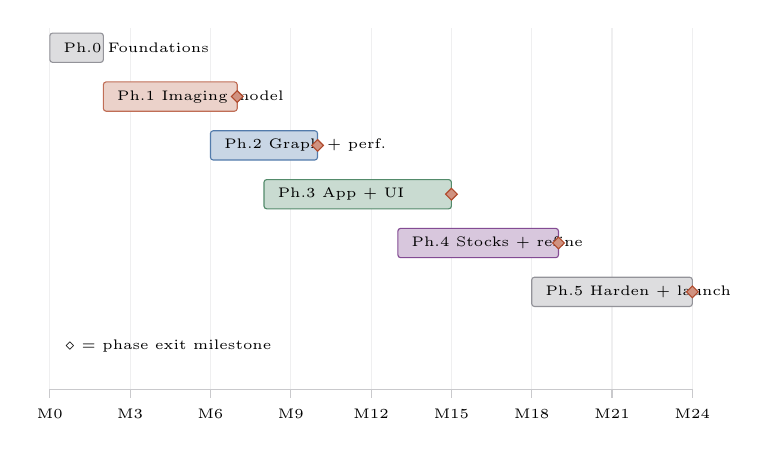
\begin{tikzpicture}[font=\scriptsize, xscale=0.34, yscale=0.62]
% axis
\draw[emLine!40] (0,0) -- (24,0);
\foreach \m in {0,3,...,24} {
  \draw[emLine!40] (\m,0) -- (\m,-0.18);
  \node[below, font=\tiny] at (\m,-0.2) {M\m};
}
\foreach \m in {0,3,...,24} \draw[emLine!12] (\m,0) -- (\m,7.4);

% bars: name / start / end / row / color
\foreach \n/\s/\e/\r/\c in {
  {Ph.0 Foundations}/0/2/6.7/emLine,
  {Ph.1 Imaging model}/2/7/5.7/emAcc,
  {Ph.2 Graph + perf.}/6/10/4.7/emBlue,
  {Ph.3 App + UI}/8/15/3.7/emGreen,
  {Ph.4 Stocks + refine}/13/19/2.7/emKey,
  {Ph.5 Harden + launch}/18/24/1.7/emLine}
{
  \draw[fill=\c!25, draw=\c!80, rounded corners=1pt] (\s,\r) rectangle (\e,\r+0.6);
  \node[right, font=\tiny, text=black] at (\s+0.15,\r+0.3) {\n};
}

% milestones
\foreach \m/\lbl/\y in {7/{AC-1..6 pass}/5.7, 10/{NFR-01..03 met}/4.7,
                        15/{feature complete}/3.7, 19/{content complete}/2.7,
                        24/{1.0 ship}/1.7}
{
  \node[diamond, draw=emAcc, fill=emAcc!60, inner sep=1.1pt] at (\m,\y+0.3) {};
}
\node[font=\tiny, anchor=west] at (0.2,0.9) {$\diamond$ = phase exit milestone};
\end{tikzpicture}
\caption{Phase schedule. Overlaps are intentional: Phase 2 begins while the imaging model is still being fitted, because graph work depends on the pipeline's \emph{shape}, which stabilizes early, not on its parameters.}
\label{fig:gantt}
\end{figure}

\subsection{Milestones and Exit Criteria}

\begin{table}[htbp]
\caption{Milestones}
\label{tab:milestones}
\begin{center}
\renewcommand{\arraystretch}{1.15}
\begin{tabularx}{\columnwidth}{@{}ll>{\raggedright\arraybackslash}X@{}}
\toprule
\textbf{M} & \textbf{Milestone} & \textbf{Exit criterion} \\
\midrule
2  & Foundations & AC-7 null test passes; CI green; device farm operational. \\
7  & Model proven & AC-1--AC-6 pass on 3 stocks; perceptual round 1 complete; discrimination rate recorded. \\
10 & Interactive & NFR-01, 02, 03 met on A15 and A17 Pro with all stages enabled. \\
15 & Feature complete & All MUST requirements implemented; accessibility audit passed. \\
19 & Content complete & 10 negative + 4 print stocks validated; all explanation content written. \\
21 & Beta & 500 testers; crash-free $\geq 99.0\%$; perceptual round 3 discrimination $< 70\%$. \\
24 & Launch & NFR-10 met; App Store review passed; day-one support ready. \\
\bottomrule
\end{tabularx}
\end{center}
\end{table}

\subsection{Team Composition}

\begin{table}[htbp]
\caption{Staffing Plan (headcount by phase)}
\label{tab:staffing}
\begin{center}
\renewcommand{\arraystretch}{1.15}
\begin{tabular}{@{}lcccccc@{}}
\toprule
\textbf{Role} & \textbf{P0} & \textbf{P1} & \textbf{P2} & \textbf{P3} & \textbf{P4} & \textbf{P5} \\
\midrule
Imaging scientist        & 1 & 2 & 1 & 1 & 2 & 1 \\
GPU / graphics engineer  & 1 & 1 & 2 & 1 & 1 & 1 \\
iOS application engineer & 1 & 1 & 1 & 3 & 3 & 3 \\
Product designer         & --- & 1 & 1 & 1 & 1 & 1 \\
QA / test engineer       & --- & --- & 1 & 1 & 1 & 2 \\
Colorist consultant (PT) & --- & 0.5 & 0.5 & 0.5 & 1 & 0.5 \\
Product lead             & 1 & 1 & 1 & 1 & 1 & 1 \\
\midrule
\textbf{Total FTE} & \textbf{4} & \textbf{6.5} & \textbf{7.5} & \textbf{8.5} & \textbf{10} & \textbf{9.5} \\
\bottomrule
\end{tabular}
\end{center}
\end{table}

The imaging scientist role is the hard hire and the schedule's critical
dependency. The required profile --- comfort with sensitometry and color science
\emph{and} the ability to implement and validate numerically --- is rare, and
the recruiting process should begin before Phase 0. The colorist consultant is
part-time throughout and is the product's connection to professional practice;
this role is what keeps the vocabulary honest.

\subsection{Cost Model}

\begin{table}[htbp]
\caption{Cost Estimate (USD, fully loaded)}
\label{tab:cost}
\begin{center}
\renewcommand{\arraystretch}{1.15}
\begin{tabular}{@{}lrr@{}}
\toprule
\textbf{Category} & \textbf{Year 1} & \textbf{Year 2} \\
\midrule
Engineering and design salaries & 1{,}420{,}000 & 1{,}760{,}000 \\
Colorist and expert consulting & 60{,}000 & 75{,}000 \\
Reference material (film, processing, scanning) & 45{,}000 & 30{,}000 \\
Densitometry and measurement equipment & 38{,}000 & 6{,}000 \\
Device farm and CI infrastructure & 34{,}000 & 22{,}000 \\
Software, tooling, developer programme & 18{,}000 & 18{,}000 \\
Legal (trademark review, privacy) & 35{,}000 & 25{,}000 \\
Beta programme and user research & 15{,}000 & 55{,}000 \\
Marketing and launch & --- & 240{,}000 \\
Contingency (12\%) & 200{,}000 & 267{,}000 \\
\midrule
\textbf{Total} & \textbf{1{,}865{,}000} & \textbf{2{,}498{,}000} \\
\bottomrule
\end{tabular}
\end{center}
\end{table}

The reference material line funds the acquisition, exposure, processing, and
drum-scanning of physical film across the shipping stock list, plus the
densitometry to measure it. It is small in absolute terms and it is the line item
that most directly determines whether AC-1 through AC-4 can be met against real
data rather than against digitized datasheet curves. It should not be cut.

\subsection{Critical Path}

The critical path runs: imaging scientist hire $\to$ characteristic curve and
print transfer $\to$ profile fitting tooling $\to$ stock library $\to$
perceptual validation $\to$ launch. Every item on it is in the imaging domain.

Three float-heavy activities can absorb schedule pressure without moving launch:
optical simulation (FR-10, SHOULD), aging module (FR-11, SHOULD), and the
pipeline inspector (FR-20, SHOULD). These are the designated cut candidates and
are marked as such in the requirements table, so that a Phase 4 slip has a
prepared response rather than an improvised one.

\subsection{Post-Launch Sequence}

\begin{table}[htbp]
\caption{Post-1.0 Release Sequence}
\label{tab:postlaunch}
\begin{center}
\renewcommand{\arraystretch}{1.15}
\begin{tabularx}{\columnwidth}{@{}ll>{\raggedright\arraybackslash}X@{}}
\toprule
\textbf{Rel.} & \textbf{Target} & \textbf{Content} \\
\midrule
1.1 & +3 mo & Stability, stock additions, user-requested workflow fixes. \\
1.2 & +6 mo & Batch processing, tethered export presets, expanded sidecar interop (CDL, CUBE export of the baked pointwise chain). \\
2.0 & +12 mo & macOS companion sharing \texttt{EmulsionCore}; iCloud recipe sync. \\
2.5 & +18 mo & Video capture with real-time emulation; Apple Log input; gate weave and breathing. \\
3.0 & +24 mo & Node-based pipeline editing; user-authored stock profiles; profile marketplace. \\
\bottomrule
\end{tabularx}
\end{center}
\end{table}

The ordering is deliberate. macOS precedes video because it reuses existing code
and reaches the P2 persona, whereas video is a substantial new engineering
programme (temporal grain coherence, real-time constraint, codec integration).
Node-based editing comes last because it is the feature that most benefits from
an established user base to design against, and because the graph infrastructure
it requires is already built (Section~\ref{sec:rendergraph}).

\section{Product Strategy and Commercial Model}
\label{sec:business}

\noindent\emph{Note on figures.} The quantities in this section are modelling
assumptions with stated bases, not measured market research. They are included
because a design document without a commercial frame cannot be evaluated for
proportionality --- an engineering programme costing \$4.4\,M must be justified
against a plausible return. Every assumption is labelled and each should be
replaced with measured data before it is used for a funding decision.

\subsection{Positioning}

\EM{} occupies a position that is currently empty: professional-grade imaging
science delivered through a consumer mobile interface. The two adjacent
positions are both crowded.

\begin{itemize}
\item \textbf{Below}: consumer film-look camera applications. Large audience,
low price, minimal technical differentiation, high churn, competition on
aesthetics and marketing rather than capability.
\item \textbf{Above}: desktop film emulation plugins. Small audience, high
price, deep technical differentiation, low churn, competition on fidelity.
\end{itemize}

The wager is that a meaningful population sits between them: people who care
enough about image quality to notice the difference and who do not have, or do
not want to use, a desktop workflow for phone captures. This population is the
P1 and P3 personas of Section~\ref{sec:requirements}.

The defensibility argument is that the gap has persisted not because it is
uninteresting but because closing it requires a combination of skills ---
sensitometry, GPU engineering, and consumer product design --- that rarely
co-occurs, and because the work does not decompose into a weekend project. That
same difficulty is the moat.

\subsection{Differentiation That Survives Copying}

Features can be copied; the following cannot easily be:

\begin{enumerate}
\item \textbf{The fitted profile library.} A stock profile is the output of
acquiring physical film, exposing calibrated wedges, processing, measuring, and
fitting. That pipeline is a capital and time investment, and it compounds: each
additional stock is cheaper than the last because the tooling amortizes.
\item \textbf{The validation apparatus.} The test suite of
Section~\ref{sec:validation} is what allows the model to be changed safely. A
competitor who copies the equations without the validation cannot iterate on
them.
\item \textbf{Architectural performance.} The $1.9\times$ from LUT baking and
tile fusion (Table~\ref{tab:optlog}) is architectural. A competitor building on
a filter-chain framework cannot reach it without rewriting.
\item \textbf{Vocabulary credibility.} If the printer lights behave like printer
lights, professionals notice and say so. That credibility is earned slowly and
is difficult to fake, because the people who would be fooled are not the people
whose opinion moves the market.
\end{enumerate}

\subsection{Commercial Model}

A hybrid model is proposed:

\begin{table}[htbp]
\caption{Proposed Pricing Structure}
\label{tab:pricing}
\begin{center}
\renewcommand{\arraystretch}{1.15}
\begin{tabularx}{\columnwidth}{@{}l l >{\raggedright\arraybackslash}X@{}}
\toprule
\textbf{Tier} & \textbf{Price} & \textbf{Contents} \\
\midrule
Free & --- & Capture, develop, export at reduced resolution. Three negative stocks, one print stock. Full pipeline, not a crippled one. \\
Pro & \$5.99/mo or \$39.99/yr & Full stock library, full resolution export, recipes, batch, sidecar interchange, all future stocks. \\
Lifetime & \$129.99 & Pro, permanently. Offered for the first twelve months only. \\
\bottomrule
\end{tabularx}
\end{center}
\end{table}

The free tier deliberately includes the \emph{complete} pipeline rather than a
reduced one. The product's argument is that physical simulation is
perceptibly better; a free tier that removes halation or grain removes the
argument. What the free tier limits is breadth (stocks) and output (resolution),
which are the dimensions a serious user needs and a casual user does not.

The lifetime option exists because a meaningful fraction of the P1/P2 population
actively resents subscriptions for creative tools, and because early lifetime
revenue funds the expensive Phase 4 profile work. Its twelve-month window
prevents it from becoming a permanent drag on recurring revenue.

\subsection{Unit Economics Model}

\begin{table}[htbp]
\caption{Illustrative Year-2 Model}
\label{tab:unitecon}
\begin{center}
\renewcommand{\arraystretch}{1.15}
\begin{tabularx}{\columnwidth}{@{}>{\raggedright\arraybackslash}X r l@{}}
\toprule
\textbf{Quantity} & \textbf{Value} & \textbf{Basis} \\
\midrule
Downloads, year 2 & 850{,}000 & Assumption \\
Free-to-paid conversion & 3.2\% & Assumption; category range 1--6\% \\
Paying users acquired & 27{,}200 & Derived \\
Annual-plan share & 62\% & Assumption \\
Blended first-year ARPU & \$34.10 & Derived \\
Gross revenue, year 2 & \$927{,}000 & Derived \\
App Store commission & 15\% & Small business programme \\
Net revenue, year 2 & \$788{,}000 & Derived \\
Year-2 cost & \$2{,}498{,}000 & Table~\ref{tab:cost} \\
\midrule
Year-2 net & $-$\$1{,}710{,}000 & Derived \\
\bottomrule
\end{tabularx}
\end{center}
\end{table}

The model does not reach breakeven in year two, and presenting it otherwise
would be dishonest. Breakeven under these assumptions occurs in year four at
approximately 78{,}000 paying users with retention above 65\%. The sensitivity
is dominated by conversion rate: a move from 3.2\% to 4.5\% pulls breakeven
forward by roughly fourteen months, while a move to 2.0\% pushes it beyond the
model's horizon.

Consequently the highest-leverage commercial activity is not acquisition volume
but conversion, and the highest-leverage conversion mechanism is the live stock
dial of Section~\ref{sec:ui} --- the moment a user sees their own image
transform under a stock they cannot access. This is a case where a product
decision and a business decision coincide exactly, and it should be instrumented
and optimized accordingly.

\subsection{Go-To-Market}

Three sequenced motions:

\paragraph{Credibility first (pre-launch, months 19--24)} Seed the product with
the professional community: colorists, cinematographers, film photographers with
audiences. The objective is not reach but verdict. If people who know what
printer lights are say the printer lights are right, that assessment propagates
through the enthusiast tier with far more force than advertising.

\paragraph{Education as marketing (launch onward)} The explanation content built
for FR-20 and the long-press affordances is genuinely useful standalone material.
Published as short articles and videos --- what a characteristic curve is, why
pushing film does not recover shadows, what halation actually is --- it
functions simultaneously as marketing, as onboarding, and as a demonstration
that the team knows the subject. This is a durable channel that does not decay
like paid acquisition.

\paragraph{Comparison content (post-launch)} Side-by-side renders against real
film scans, published with the source files. This is only available to a product
confident in its fidelity, which is precisely why it is persuasive.

\subsection{Risks to the Commercial Thesis}

The commercial risks are distinct from the engineering risks of
Section~\ref{sec:risks} and are enumerated there alongside them. The dominant
one is stated here because it shapes strategy: \textbf{the population that can
perceive the difference may be smaller than assumed}. If most users cannot
distinguish a physically simulated render from a good LUT at phone viewing size,
the product's entire investment thesis is mispriced.

The mitigation is measurement, early. The perceptual evaluation of
Section~\ref{sec:validation} should be extended during Phase 1 to include a
non-expert cohort, testing not whether they can identify real film but whether
they \emph{prefer} the physically simulated render to a strong LUT baseline. A
preference rate near chance among non-experts would be a signal to reposition
toward the professional tier and price accordingly, and it is far better to
learn that in month seven than in month twenty-four.

\section{Risk Register}
\label{sec:risks}

\subsection{Method}

Each risk is scored on likelihood $L$ and impact $I$, both $1$--$5$, with
exposure $E = L \times I$. Risks with $E \geq 12$ require an owner, a named
mitigation, and a trigger condition that converts the mitigation into action.
Risks are reviewed at every phase boundary.

\subsection{Technical Risks}

\begin{table}[htbp]
\caption{Technical Risk Register}
\label{tab:techrisk}
\begin{center}
\renewcommand{\arraystretch}{1.15}
\begin{tabularx}{\columnwidth}{@{}l>{\raggedright\arraybackslash}Xccc@{}}
\toprule
\textbf{ID} & \textbf{Risk} & $L$ & $I$ & $E$ \\
\midrule
T-01 & Reference sensitometric data is unavailable or inconsistent for target stocks, preventing AC-1 validation. & 4 & 5 & 20 \\
T-02 & Model is numerically correct but perceptually unconvincing; discrimination rate stays high. & 3 & 5 & 15 \\
T-03 & Apple changes \texttt{CIRAWFilter} behavior so that scene-referred decode is no longer achievable. & 2 & 5 & 10 \\
T-04 & Performance targets unreachable on A14/A15, forcing a raised minimum device. & 2 & 4 & 8 \\
T-05 & Memory budget exceeded on 6\,GB devices during export, causing jetsam. & 3 & 4 & 12 \\
T-06 & Grain lattice produces visible aliasing at some format/resolution combinations. & 3 & 3 & 9 \\
T-07 & Profile version migration silently changes users' existing edits. & 2 & 5 & 10 \\
T-08 & Device calibration constant $g_{\mathrm{cal}}$ varies within a device model, breaking the exposure anchor. & 2 & 4 & 8 \\
T-09 & Halation pyramid produces visible seams at ROI tile boundaries under extreme radii. & 3 & 3 & 9 \\
T-10 & Thermal throttling makes sustained editing unpleasant on older devices. & 3 & 3 & 9 \\
\bottomrule
\end{tabularx}
\end{center}
\end{table}

\paragraph{T-01 (E = 20), owner: imaging scientist}
The highest-exposure technical risk. Published sensitometric data varies in
completeness; some stocks publish full $D$--$\logE$ families, others publish
only a summary. Digitizing a printed curve introduces its own error.

\emph{Mitigation.} Budget for physical measurement (Table~\ref{tab:cost}):
acquire film, expose calibrated step wedges under controlled conditions, process
at a professional laboratory with documented chemistry, and measure with a
transmission densitometer. This produces primary data. \emph{Trigger:} if by
month 4 fewer than six of the ten target stocks have data adequate for AC-1
validation, reduce the launch stock list to those that do and reallocate. A
smaller library of stocks that are demonstrably correct is a better product than
a larger library of guesses, and it is a better story.

\paragraph{T-02 (E = 15), owner: product lead}
It is entirely possible to build a model that matches every measurement and
still produces images that do not read as film, because the cues the eye uses may
not be the ones measured. This is the risk that the whole enterprise is
subtly aimed at the wrong target.

\emph{Mitigation.} The cue-elicitation protocol in
Section~\ref{sec:validation}: the panel names what tipped them off, and that list
drives development priority. \emph{Trigger:} if round-2 discrimination exceeds
80\% and the cue list is dominated by a phenomenon not in the model, escalate to
a model extension decision at the phase boundary rather than continuing to
refine existing stages.

\paragraph{T-05 (E = 12), owner: GPU engineer}
Table~\ref{tab:memory} shows an 878\,MB peak against a 900\,MB budget. That is
not enough margin.

\emph{Mitigation.} Export tiling is implemented in v1.0 rather than deferred,
and the tiling threshold is set conservatively --- tiling engages whenever the
projected live set exceeds 600\,MB, not 900\,MB. Additionally, the decoded
source is released before the encode staging buffer is allocated, which the
naive ordering does not do. \emph{Trigger:} any jetsam observed during Phase 2
device testing forces the tiling threshold down a further 100\,MB.

\subsection{Product and Market Risks}

\begin{table}[htbp]
\caption{Product Risk Register}
\label{tab:prodrisk}
\begin{center}
\renewcommand{\arraystretch}{1.15}
\begin{tabularx}{\columnwidth}{@{}l>{\raggedright\arraybackslash}Xccc@{}}
\toprule
\textbf{ID} & \textbf{Risk} & $L$ & $I$ & $E$ \\
\midrule
P-01 & The addressable audience for physical accuracy is smaller than modelled; conversion falls below 2\%. & 3 & 5 & 15 \\
P-02 & The laboratory vocabulary is a barrier rather than a differentiator for the P3 persona. & 3 & 4 & 12 \\
P-03 & A well-resourced competitor ships an adequate approximation first and defines the category. & 3 & 4 & 12 \\
P-04 & Apple ships comparable film simulation as a system feature. & 2 & 5 & 10 \\
P-05 & Trademark or brand objection to descriptive use of stock names. & 3 & 3 & 9 \\
P-06 & Subscription fatigue suppresses conversion regardless of quality. & 3 & 3 & 9 \\
\bottomrule
\end{tabularx}
\end{center}
\end{table}

\paragraph{P-01 (E = 15)}
Addressed in Section~\ref{sec:business}. The mitigation is early measurement
with a non-expert cohort during Phase 1, and the prepared response is
repositioning toward the professional tier with adjusted pricing, which the
architecture supports without rework.

\paragraph{P-02 (E = 12), owner: product designer}
The vocabulary is a core commitment, and abandoning it would hollow out the
product. But if a user cannot find the brightness control because it is called
print density, the commitment has failed in execution rather than in principle.

\emph{Mitigation.} The explanation affordance (long-press) is not optional
polish; it is the mechanism that makes the vocabulary teachable, and it is
scheduled in Phase 4 with dedicated content authoring. Additionally, search
within the develop workspace accepts colloquial terms and navigates to the
corresponding laboratory control, showing both names --- this teaches rather
than aliases. \emph{Trigger:} if beta task-completion testing shows more than
25\% of P3-persona users failing to locate a lightness control within 60
seconds, add a first-run guided tour before ship.

\paragraph{P-05 (E = 9), owner: product lead}
Film stock names are used descriptively to identify a modelled response, which
is a recognized nominative use, and no proprietary profile data is
redistributed (CR-04). Nonetheless the risk is nonzero.

\emph{Mitigation.} Legal review before launch (budgeted). A prepared fallback
naming scheme exists in which each profile carries a descriptive name
("Daylight Portrait 400") with the reference stock identified only in the
profile's technical notes. The fallback is designed now, so that adopting it
later is a data change and not an engineering change.

\subsection{Programme Risks}

\begin{table}[htbp]
\caption{Programme Risk Register}
\label{tab:progrisk}
\begin{center}
\renewcommand{\arraystretch}{1.15}
\begin{tabularx}{\columnwidth}{@{}l>{\raggedright\arraybackslash}Xccc@{}}
\toprule
\textbf{ID} & \textbf{Risk} & $L$ & $I$ & $E$ \\
\midrule
G-01 & Imaging scientist role cannot be filled, or is filled late. & 4 & 5 & 20 \\
G-02 & Phase 1 overruns, compressing everything downstream. & 4 & 4 & 16 \\
G-03 & Scope expansion into video before v1.0 ships. & 3 & 4 & 12 \\
G-04 & Key-person dependency on the GPU architecture. & 3 & 4 & 12 \\
\bottomrule
\end{tabularx}
\end{center}
\end{table}

\paragraph{G-01 (E = 20), owner: product lead}
The single highest-exposure risk in the programme. The required skill
combination is scarce.

\emph{Mitigation.} Begin recruiting before Phase 0. Structure the role to be
fillable by two adjacent profiles working together --- a color scientist without
strong implementation skills paired with an engineer without domain background
--- since that pair is far easier to hire than the unicorn. Engage the colorist
consultant early to provide domain review in the interim. \emph{Trigger:} if the
role is unfilled at month 2, activate the pair structure and extend Phase 1 by
six weeks in the plan of record rather than absorbing the slip silently.

\paragraph{G-02 (E = 16)}
Phase 1 is already given twice an optimistic estimate, which is the primary
mitigation. The secondary mitigation is the designated cut list in
Section~\ref{sec:roadmap} (optical, aging, inspector), which provides
approximately ten weeks of recoverable schedule in later phases without touching
any MUST requirement.

\paragraph{G-04 (E = 12)}
The render graph is subtle and, written by one person, becomes a bus factor of
one.

\emph{Mitigation.} The graph's design is documented in
Section~\ref{sec:rendergraph} at implementation detail, its properties are
enforced by the property-based tests of V-18 through V-20, and a second engineer
is assigned to Phase 2 explicitly for knowledge distribution rather than
throughput.

\subsection{Risk Summary}

\begin{table}[htbp]
\caption{Top Risks by Exposure}
\label{tab:toprisk}
\begin{center}
\renewcommand{\arraystretch}{1.15}
\begin{tabular}{@{}llc@{}}
\toprule
\textbf{ID} & \textbf{Risk} & $E$ \\
\midrule
T-01 & Reference data unavailable & 20 \\
G-01 & Imaging scientist hire & 20 \\
G-02 & Phase 1 overrun & 16 \\
T-02 & Perceptually unconvincing & 15 \\
P-01 & Audience smaller than modelled & 15 \\
\bottomrule
\end{tabular}
\end{center}
\end{table}

Four of the top five risks concern the imaging model or the people who build it.
That concentration is not a defect of the analysis; it is the accurate shape of
this programme, and it is the reason the schedule, the budget, and the staffing
plan all front-load the same area.

\section{Future Directions}
\label{sec:future}

This section specifies deferred capabilities at architectural depth --- enough
to confirm that the v1.0 design does not foreclose them, and to identify the
specific v1.0 decisions that were made to keep them open.

\subsection{Video and Real-Time Emulation}

\paragraph{What changes} The pipeline becomes a per-frame operation at 24, 25,
or 30\,fps, with a hard budget of 33\,ms shared with capture, encode, and audio.
The pointwise chain is already a single LUT fetch and is essentially free. The
binding costs are halation (0.44\,ms at preview resolution on A17, but video is
captured at higher resolution) and grain.

\paragraph{The hard problem} Temporal grain coherence. Grain must be
\emph{uncorrelated} between frames --- real grain is a new realization each
frame --- but the underlying image is correlated, so naive per-frame
regeneration produces the correct result. The genuine difficulty is that video
codecs allocate bits to changing regions, and uncorrelated full-frame noise
consumes the entire bitrate. Professional practice is to grade with grain and
deliver at a bitrate sufficient to carry it; on a phone this is a real
constraint.

The specified approach is to record the grain \emph{parameters} in the container
alongside a clean encode, and synthesize grain at playback within the
application, with a baked-in option for export. This is architecturally
identical to the film grain synthesis facility standardized in AV1, and the v1.0
decision that makes it possible is that grain is fully determined by
(seed, parameters, film coordinate) --- Section~\ref{sec:grain} --- so it can be
regenerated exactly from a handful of bytes.

\paragraph{v1.0 decisions that preserve this} Resolution-independent,
seed-deterministic grain; physical-unit specification of all spatial phenomena;
the render graph's resolution-relative descriptors.

\subsection{Log Input and Professional Interchange}

Apple Log and Blackmagic Log inputs require only an additional input transform:
a log-to-linear decode followed by the existing $\mathbf{M}_{\mathrm{in}}$. The
pipeline is already scene-referred, which is the property that makes this a
small change rather than a redesign.

Export of the baked pointwise chain as a \texttt{.cube} 3D LUT is likewise
nearly free --- the LUT already exists (Section~\ref{sec:lutbake}) and needs
only serialization plus a documented shaper. This is a high-value, low-cost
feature for the P2 persona: it lets a colorist take an \EM{} grade into
Resolve directly. It is scheduled for 1.2.

The honest caveat, which must be surfaced in the UI when exporting a LUT: the
spatial and stochastic stages cannot be baked. A \texttt{.cube} export carries
the color science and none of the halation, grain, or interlayer effects, and
telling the user so is more valuable than a silently incomplete export.

\subsection{ACES Integration}

The working space is already ACEScg. Full ACES integration adds: IDT selection
for non-Apple sources, an ACES container output (OpenEXR with the appropriate
metadata), and --- the substantive part --- a decision about where the film
model sits relative to the ACES viewing transform.

The correct answer is that \EM{}'s negative-plus-print chain \emph{is} an
output transform: it takes scene-referred data to display-referred, which is
exactly the RRT+ODT's role. \EM{} therefore replaces the ACES output transform
rather than composing with it, and an ACES-integrated build must expose that
choice explicitly rather than silently double-transforming. This is stated here
because it is the mistake that ACES integrations most commonly make.

\subsection{Node-Based Pipeline Editing}

The render graph is already a DAG with declared reads, writes, and parameter
dependencies (Section~\ref{sec:rendergraph}). Node-based editing requires: a
serialized graph topology in the recipe rather than a fixed chain; a UI for
constructing it; validation that user-constructed graphs are acyclic and
domain-consistent (a pass consuming density must not be fed linear exposure);
and a defined behavior for graphs whose stages appear in a physically impossible
order.

That last item is the interesting design problem, and it is a direct conflict
with the parameter-honesty principle. The proposed resolution is that arbitrary
ordering is permitted but non-physical orderings are marked in the interface,
with an explanation of what the physical ordering would be. Freedom with
labelling, rather than prohibition or silence.

\subsection{User-Authored and Community Profiles}

The stock profile format is already a versioned JSON parameter block
(Section~\ref{sec:schema}). Opening it requires: a profile editor exposing the
parameters that are currently profile-only ($\mathbf{A}$, $\mathbf{C}$, grain
$\sigma_1$/$\chi$, halation $\ell$ and $\boldsymbol{\beta}$); a validator
enforcing the well-formedness condition \eqref{eq:wellformed} and the
monotonicity requirement AC-6; and a distribution mechanism.

The genuinely valuable version of this feature is not authoring by eye but
\emph{fitting from measurement}: a user photographs a step wedge on their own
film, scans it, and the application fits $\theta$. That is a substantially more
defensible feature and it aligns with the product's identity. It requires a
guided capture flow and a robust fitter, and it is the correct 3.0 headline
feature.

\subsection{Machine Learning: Where It Helps and Where It Does Not}

The original proposal contemplates machine learning for exposure recommendation
and for estimating spectral film responses from scanned negatives. These are
very different propositions and should be evaluated separately.

\paragraph{Estimating model parameters from scans --- promising} Fitting
$\theta$, $\mathbf{A}$, $\mathbf{C}$, and the grain parameters from a set of
scanned reference images is a well-posed inverse problem. Because the forward
model of Sections~\ref{sec:negative}--\ref{sec:grain} is differentiable by
construction (this is why the softplus formulation was chosen over a spline),
gradient-based optimization applies directly, and the "learning" is parameter
estimation within a physical model rather than a black box. The result remains
interpretable, editable, and validatable against AC-1. This is the right use.

\paragraph{End-to-end learned film emulation --- rejected} A network mapping
RAW to film-look output would discard every property the product is built on:
interpretability, parameter honesty, controllability, and the ability to
validate. It would also be immediately commoditized. This direction is
explicitly not pursued.

\paragraph{Exposure and stock recommendation --- modest} A small on-device
model suggesting exposure compensation and stock from scene content is a
convenience feature with real but bounded value. It should be additive and
always overridable, and it should present its reasoning in the product's own
vocabulary ("this scene has a 9-stop range; a stock with a longer straight line
will hold both ends").

\subsection{Full Spectral Rendering}

The reduced spectral strategy of Section~\ref{sec:colorspace} bakes crosstalk at
profile time against a reference illuminant. A full spectral path would carry
$N \approx 31$ wavelength samples through the exposure and density stages,
integrating against measured layer sensitivities and dye transmittances.

The cost is roughly $10\times$ in the density stage --- which, per
Table~\ref{tab:previewperf}, is a small fraction of the total, so the cost is
more tolerable than it first appears. The real obstacle is data: measured
spectral sensitivities and dye densities are not published for most stocks and
would require spectrophotometric measurement of physical samples.

The value would be correct rendering under unusual illuminants and correct
prediction of crosstalk from first principles rather than by fitted matrix.
This is a research direction rather than a product feature, appropriate for a
later phase once the profile measurement apparatus already exists for other
reasons.

\subsection{Cross-Device Continuity}

The macOS companion shares \texttt{EmulsionCore} and \texttt{EmulsionRender}
unchanged; only \texttt{EmulsionCapture} and the UI layer differ. This is the
direct payoff of the module layering in Table~\ref{tab:layers} and the reason
that layering was specified as strictly as it was.

Synchronization carries recipes and library metadata, not images. A recipe is
under a kilobyte; syncing recipes is trivial and syncing 48\,MP originals is a
different product with different economics. The sync model is therefore:
recipes and metadata via CloudKit, images by user action only. This keeps the
privacy commitment of CR-02 substantially intact --- the default remains that
no image leaves the device.

\section{Conclusion}

\subsection{What This Document Specifies}

\EM{} is specified here as a mobile application that treats a photograph as a
latent image awaiting development rather than as a finished picture awaiting a
filter. The specification is complete enough to build from: the imaging model is
given in closed form with numerical defaults and validation tolerances; the GPU
architecture is given with the fusion strategy, precision policy, and memory
budget that make it meet its latency targets; the application architecture,
interface, and persistence schema are given at implementation detail; and the
programme is given with phases, staffing, cost, and a risk register that names
owners and triggers.

The technical argument reduces to a single structural claim. A lookup table is a
pointwise function, and the phenomena that identify photographic film ---
halation, grain, interlayer inhibition, shoulder compression of scene highlights
--- are not pointwise. They are spatial, stochastic, or dependent on radiometric
information that a display-referred image no longer contains. No amount of
refinement to a pointwise operator on a rendered image closes that gap, because
the gap is one of representational class rather than of quality.

Carrying scene-referred data through a chain of physically motivated transforms
does close it, and the performance analysis in
Section~\ref{sec:performance} shows that doing so costs 2\,ms of GPU time per
preview frame on current mobile silicon. The obstacle was never computational.

\subsection{What Would Falsify It}

A design document that cannot be wrong is not a design document. Three concrete
outcomes would invalidate the approach as specified:

\begin{enumerate}
\item \textbf{The measurements do not close.} If AC-1 through AC-4 cannot be
met for a majority of target stocks with available or obtainable reference data,
then the model is being fitted to guesses and its claim to physical grounding is
rhetorical. Risk T-01, checked at month 4.
\item \textbf{Correctness does not produce conviction.} If the perceptual panel
continues to identify the renders reliably while every numerical acceptance
criterion passes, the model is measuring the wrong things. Risk T-02, checked at
month 7 and again at month 15.
\item \textbf{The distinction does not matter commercially.} If non-expert users
show no preference between a physically simulated render and a strong LUT
baseline, the product is correctly built and incorrectly aimed. Risk P-01,
checked during Phase 1.
\end{enumerate}

Each has a defined trigger and a prepared response. That is the difference
between a plan and an intention.

\subsection{The Argument in One Sentence}

Every quantity in this document that a user can adjust corresponds to something
that exists in a photographic laboratory, and every equation that consumes those
quantities can be checked against a densitometer. If both remain true through
implementation, the product's claim is not a marketing position but a
verifiable property --- and a photograph made with it will not have been
filtered. It will have been developed.


\appendices
\section{Stock Profile Parameter Reference}
\label{app:stockparams}

This appendix is the normative parameter reference for the shipping profile
bundle. Every number here is consumed by an equation in the body, and every
equation in the body that requires a stock-specific constant draws it from
here. The tables are the authoritative source; the profile JSON files in the
application bundle are generated from them by the profile-fitting tool, never
hand-edited.

\subsection{Status of These Values}

The values are \emph{provisional fits}. Those marked \textbf{M} in
Table~\ref{tab:provenance} are least-squares fits to published sensitometric
data and are expected to satisfy AC-1 without further work; those marked
\textbf{P} are partial fits in which some parameters are inherited from a
family default because published data is incomplete; those marked \textbf{E}
are engineering estimates awaiting the measurement campaign of
Section~\ref{sec:roadmap}. A stock does not ship until it reaches \textbf{M}
and passes AC-1 (Section~\ref{sec:validation}); this is the mitigation for
risk T-01.

\subsection{Units and Conventions}

\begin{itemize}
\item Densities are Status M diffuse densities for negative stocks and
Status A for print stocks, per ISO 5-3 geometry.
\item Log exposures $x = \logE$ are in $\log_{10}$ lux-seconds at the film
plane, so ISO speed follows from \eqref{eq:speedpoint} rather than being
carried separately. The scene-to-film mapping is \eqref{eq:isoshift}.
\item All spatial parameters are micrometres at the film plane and are
converted to pixels by \eqref{eq:formatscale} at render time.
\item Reversal stocks carry $\gamma < 0$. The characteristic curve
\eqref{eq:charcurve} is unchanged --- $\softp{a}{\cdot}$ is monotone in $u$, and
$u = \gamma(x - x_0)$ is decreasing when $\gamma < 0$, so density decreases with
exposure as a positive image requires. The well-formedness test
\eqref{eq:wellformed} is applied to $|\gamma|$, and the sign of the speed-point
offset in \eqref{eq:speedpoint} inverts accordingly. Reversal stocks default to
the bypass print profile, because a transparency is viewed directly.
\end{itemize}

\subsection{Parameter Inventory}

Table~\ref{tab:paraminventory} lists every stock-carried parameter, the
equation that consumes it, and whether it is per-record or scalar. A profile
that omits a parameter inherits its family default; a profile that carries a
parameter not in this table fails validation at load.

\begin{table}[htbp]
\caption{Stock Profile Parameter Inventory}
\label{tab:paraminventory}
\begin{center}
\renewcommand{\arraystretch}{1.12}
\footnotesize
\begin{tabularx}{\columnwidth}{@{}llc>{\raggedright\arraybackslash}X@{}}
\toprule
\textbf{Symbol} & \textbf{Eq.} & \textbf{Rec.} & \textbf{Quantity} \\
\midrule
$\Dmin$        & \eqref{eq:charcurve}   & \checkmark & Base + fog density \\
$\Delta D$     & \eqref{eq:charcurve}   & \checkmark & Density range \\
$\gamma$       & \eqref{eq:ucoord}      & \checkmark & Straight-line gamma \\
$x_0$          & \eqref{eq:ucoord}      & \checkmark & Extrapolated speed point \\
$\kappa_t$     & \eqref{eq:charcurve}   & \checkmark & Toe softness \\
$\kappa_s$     & \eqref{eq:charcurve}   & \checkmark & Shoulder softness \\
$m$            & \eqref{eq:maskdepletion} & \checkmark & Mask depletion \\
$\Delta x^{\mathrm{(bal)}}$ & \eqref{eq:tungsten} & \checkmark & Layer speed balance \\
$\mathbf{w}_{\mathrm{spectral}}$ & \eqref{eq:pan} & --- & Panchromatic weights \\
$\gamma_\infty/\gamma^{(0)}$ & \eqref{eq:gammatime} & --- & Development ceiling \\
$\phi_0, \beta_f$ & \eqref{eq:fog}      & \checkmark & Fog growth \\
$\alpha_s$     & \eqref{eq:speedshift}  & --- & Speed recovery \\
$\tau_t, \tau_D$ & Sec.~\ref{sec:development} & --- & Toe / range drift \\
$\mathbf{A}$   & \eqref{eq:dirmatrix}   & $3{\times}3$ & DIR coupling \\
$\sigma_1^{\mathrm{DIR}}, \sigma_2^{\mathrm{DIR}}, w_2$ & \eqref{eq:twoscale} & --- & Diffusion scales \\
$\mu$          & \eqref{eq:activityweight} & --- & Activity exponent \\
$G_S$          & \eqref{eq:selwyn}      & \checkmark & Selwyn granularity \\
$\sigma_1^{g}, \chi, \zeta$ & \eqref{eq:grainkernel} & --- & Grain kernel \\
$\nu_1, \nu_2$ & \eqref{eq:grainvar}    & --- & Granularity shape \\
$\varphi$      & \eqref{eq:graincorr}   & --- & Grain chroma correlation \\
$\alpha_h, \ell_R, \omega$ & \eqref{eq:halpsf} & --- & Halation \\
$\boldsymbol{\beta}$ & Tab.~\ref{tab:halparams} & \checkmark & Halation bias \\
$\mathbf{C}$   & \eqref{eq:cmatrix}     & $3{\times}3$ & Printing density \\
$\mathbf{D}'_{\mathrm{aim}}$ & \eqref{eq:aimbalance} & \checkmark & Print aim density \\
\bottomrule
\end{tabularx}
\end{center}
\end{table}

\subsection{Negative Characteristic Curve Parameters}

Table~\ref{tab:negparams} gives the green-record parameters of
\eqref{eq:charcurve} for the ten launch stocks at the manufacturer's normal
process ($A = 1$). The red and blue records are obtained by applying the
per-record offsets of Table~\ref{tab:recordoffsets}; this factoring is used
rather than thirty independent numbers because the offsets are structurally
similar across a stock family and because crossover --- non-parallelism of the
three records --- is then an explicit, reviewable quantity rather than an
accident of three separate fits.

\begin{table*}[htbp]
\caption{Green-Record Characteristic Curve Parameters at Normal Process}
\label{tab:negparams}
\begin{center}
\renewcommand{\arraystretch}{1.15}
\footnotesize
\begin{tabular}{@{}llrrrrrrrl@{}}
\toprule
\textbf{Profile ID} & \textbf{Display name} & \textbf{ISO} & $\gamma_G$ & $\Delta D_G$ & $x_{0,G}$ & $\kappa_{t,G}$ & $\kappa_{s,G}$ & $\Dmin{}_{,G}$ & \textbf{Process} \\
\midrule
\texttt{neg.portra160}  & Portra 160-type       & 160 & $\phantom{-}0.58$ & $1.86$ & $-2.31$ & $0.155$ & $0.115$ & $0.90$ & C-41 \\
\texttt{neg.portra400}  & Portra 400-type       & 400 & $\phantom{-}0.63$ & $1.90$ & $-2.71$ & $0.140$ & $0.110$ & $0.92$ & C-41 \\
\texttt{neg.gold200}    & Gold 200-type         & 200 & $\phantom{-}0.68$ & $1.78$ & $-2.41$ & $0.150$ & $0.098$ & $0.88$ & C-41 \\
\texttt{neg.ektar100}   & Ektar 100-type        & 100 & $\phantom{-}0.72$ & $2.02$ & $-2.11$ & $0.128$ & $0.092$ & $0.86$ & C-41 \\
\texttt{neg.superia400} & Superia 400-type      & 400 & $\phantom{-}0.65$ & $1.84$ & $-2.71$ & $0.145$ & $0.104$ & $0.94$ & C-41 \\
\texttt{neg.v3\_500t}   & Vision3 500T-type     & 500 & $\phantom{-}0.55$ & $2.06$ & $-2.81$ & $0.168$ & $0.130$ & $0.96$ & ECN-2 \\
\texttt{rev.velvia50}   & Velvia 50-type        & 50  & $-1.95$           & $3.10$ & $-1.80$ & $0.090$ & $0.140$ & $0.10$ & E-6 \\
\texttt{rev.provia100}  & Provia 100F-type      & 100 & $-1.72$           & $2.95$ & $-2.10$ & $0.105$ & $0.150$ & $0.09$ & E-6 \\
\texttt{mono.trix400}   & Tri-X 400-type        & 400 & $\phantom{-}0.62$ & $1.92$ & $-2.71$ & $0.160$ & $0.200$ & $0.22$ & B\&W \\
\texttt{mono.hp5}       & HP5 Plus-type         & 400 & $\phantom{-}0.58$ & $1.88$ & $-2.71$ & $0.170$ & $0.215$ & $0.20$ & B\&W \\
\bottomrule
\multicolumn{10}{@{}p{\textwidth}@{}}{\footnotesize Every row satisfies the well-formedness constraint \eqref{eq:wellformed}, $\Delta D \geq 4(\kappa_t + \kappa_s)$, with the smallest margin at \texttt{mono.hp5} ($1.88$ against a required $1.54$) --- monochrome stocks sit closest to the bound because their long shoulders demand a large $\kappa_s$, which is also why the constraint binds first there when a user pushes development. Monochrome stocks carry a single record and the $G$ column is the whole profile; the panchromatic weights of \eqref{eq:pan} are $(0.30, 0.59, 0.11)$ for both, with the orthochromatic variant $(0.02, 0.68, 0.30)$ available as a process option.}
\end{tabular}
\end{center}
\end{table*}

\begin{table}[htbp]
\caption{Per-Record Offsets Relative to the Green Record}
\label{tab:recordoffsets}
\begin{center}
\renewcommand{\arraystretch}{1.15}
\footnotesize
\begin{tabular}{@{}lrrrrrr@{}}
\toprule
& \multicolumn{2}{c}{\textbf{Color negative}} & \multicolumn{2}{c}{\textbf{Transparency}} & \multicolumn{2}{c}{\textbf{Mono}} \\
\cmidrule(lr){2-3}\cmidrule(lr){4-5}\cmidrule(lr){6-7}
\textbf{Offset} & $R$ & $B$ & $R$ & $B$ & $R$ & $B$ \\
\midrule
$\Delta\gamma$      & $-0.02$ & $+0.03$ & $-0.06$ & $+0.08$ & --- & --- \\
$\Delta(\Delta D)$  & $+0.05$ & $-0.05$ & $+0.04$ & $-0.07$ & --- & --- \\
$\Delta x_0$        & $-0.05$ & $+0.05$ & $-0.03$ & $+0.04$ & --- & --- \\
$\Delta\kappa_t$    & $+0.010$ & $-0.010$ & $+0.008$ & $-0.006$ & --- & --- \\
$\Delta\kappa_s$    & $+0.010$ & $\phantom{+}0.000$ & $+0.006$ & $-0.004$ & --- & --- \\
$\Dmin$ (absolute)  & $0.58$ & $1.28$ & $0.11$ & $0.12$ & --- & --- \\
$m$ (mask depl.)    & $0.00$ & $0.10$ & $0.00$ & $0.00$ & --- & --- \\
\bottomrule
\multicolumn{7}{@{}p{0.95\columnwidth}@{}}{\footnotesize The $\Dmin$ row is absolute, not an offset, because it is the orange mask and is the one quantity that must be read directly. The green-record value is in Table~\ref{tab:negparams}; $m_G = 0.06$. Transparency stocks have no mask, so their $\Dmin$ spread is only base tint.}
\end{tabular}
\end{center}
\end{table}

The small $\Delta\gamma$ values are deliberate: three records with identical
gamma have no crossover at all, which is unrealistically clean, while the
$\pm 0.03$ spread here reproduces the mild crossover that makes a real negative
resist a single global balance correction in deep shadow. Transparency stocks
carry roughly three times the spread, which is why slide film is unforgiving of
mixed lighting.

\subsection{Tungsten Balance}

\texttt{neg.v3\_500t} is the only launch stock with a non-zero layer speed
balance in \eqref{eq:tungsten}:

\begin{equation}
\Delta x^{\mathrm{(bal)}}_{\mathrm{v3\_500t}} = (-0.29,\; 0.00,\; +0.42)^\top ,
\end{equation}

derived from the ratio of layer sensitivities integrated against a 3200\,K
Planckian SPD versus D55. Shot under daylight without an 85B correction, this
places the blue record $0.42$ in log exposure higher and the red record $0.29$
lower, which drives blue toward its shoulder in bright areas while red sits in
its toe --- producing a cast that changes character with luminance rather than
a uniform tint. Shipping values for the remaining balance and white-balance
constants are in Table~\ref{tab:balance}.

\subsection{Chemistry and Development}

The chemistry profiles of Table~\ref{tab:chemistry} supply $(\gamma_\infty /
\gamma^{(0)}, \phi_0, \beta_f, \alpha_s, \rho)$. Stocks override only where
their measured push response departs from the family, and carry a per-record
fog coefficient vector because the blue-sensitive layer fogs fastest:

\begin{equation}
\boldsymbol{\phi}_0 / \phi_0 = (0.82,\; 1.00,\; 1.34)
\end{equation}

for all C-41 and ECN-2 stocks, $(0.90, 1.00, 1.15)$ for E-6, and unity for
monochrome. The remaining development constants are family-wide: $\tau_t =
0.30$, $\tau_D = 0.12$, $E_a/R = 8.4\times10^{3}$\,K, $t_0 = 195$\,s at $T_0 =
311.15$\,K (38\,\textdegree C) for C-41, $t_0 = 180$\,s at $314.65$\,K
(41.5\,\textdegree C) for E-6 first development, and $t_0 = 180$\,s at
$314.75$\,K (41.6\,\textdegree C) for ECN-2. Agitation efficiency uses
$\eta_\infty = 1.22$, $\eta_0 = 0.61$, $a_c = 0.85$.

\subsection{Interlayer Inhibition}

The color negative coupling matrix is \eqref{eq:dirmatrix}. Per-stock variation
is carried as a scalar multiplier on $\mathbf{A}$ rather than as ten
independent matrices, because the published data does not support
distinguishing the individual entries and pretending otherwise would be
dishonest about the fit quality:

\begin{center}
\renewcommand{\arraystretch}{1.1}
\footnotesize
\begin{tabular}{@{}lrrr@{}}
\toprule
\textbf{Family} & \textbf{$\mathbf{A}$ scale} & $\sigma_1$ ($\mu$m) & $\sigma_2$ ($\mu$m) \\
\midrule
Portra-type (low contrast, high DIR) & $1.15$ & $1.2$ & $6.0$ \\
Consumer color negative              & $0.85$ & $1.3$ & $6.5$ \\
Saturated color negative             & $1.30$ & $1.1$ & $5.5$ \\
Motion picture negative              & $1.20$ & $1.2$ & $6.2$ \\
Transparency                         & $0.40$ & $1.0$ & $4.5$ \\
Monochrome (scalar $a = 0.34$)       & $1.00$ & $1.4$ & $7.0$ \\
\bottomrule
\end{tabular}
\end{center}

\noindent with $w_2 = 0.38$ and $\mu = 1.0$ throughout. Agitation modulates
$\sigma_2$ and $w_2$ inversely per Section~\ref{sec:interlayer}; at the minimum
agitation setting $\sigma_2$ reaches $1.9\times$ its nominal value and $w_2$
reaches $0.55$, which is the stand-development limit.

\subsection{Grain Parameters}

\begin{table*}[htbp]
\caption{Grain Synthesis Parameters}
\label{tab:grainparams}
\begin{center}
\renewcommand{\arraystretch}{1.15}
\footnotesize
\begin{tabular}{@{}lrrrrrrl@{}}
\toprule
\textbf{Profile ID} & $G_S \times 10^{3}$ & $\sigma_1^{g}$ ($\mu$m) & $\chi$ & $\zeta$ & $\varphi$ & $(\nu_1, \nu_2)$ & \textbf{Mode at 1:1} \\
\midrule
\texttt{neg.portra160}  & $3.0$  & $0.85$ & $0.12$ & $3.0$ & $0.15$ & $(1.00, 1.00)$ & Gaussian \\
\texttt{neg.portra400}  & $4.0$  & $1.05$ & $0.16$ & $3.0$ & $0.15$ & $(1.00, 1.00)$ & Gaussian \\
\texttt{neg.gold200}    & $5.5$  & $1.10$ & $0.20$ & $3.2$ & $0.18$ & $(1.00, 0.92)$ & Gaussian \\
\texttt{neg.ektar100}   & $3.4$  & $0.80$ & $0.10$ & $2.8$ & $0.12$ & $(1.00, 1.00)$ & Gaussian \\
\texttt{neg.superia400} & $4.2$  & $1.02$ & $0.18$ & $3.0$ & $0.16$ & $(1.00, 0.96)$ & Gaussian \\
\texttt{neg.v3\_500t}   & $5.0$  & $1.15$ & $0.17$ & $3.1$ & $0.14$ & $(1.00, 1.00)$ & Gaussian \\
\texttt{rev.velvia50}   & $9.0$  & $0.95$ & $0.14$ & $2.9$ & $0.35$ & $(1.00, 0.80)$ & Gaussian \\
\texttt{rev.provia100}  & $8.0$  & $0.98$ & $0.15$ & $2.9$ & $0.35$ & $(1.00, 0.84)$ & Gaussian \\
\texttt{mono.trix400}   & $17.0$ & $1.55$ & $0.28$ & $3.4$ & $1.00$ & $(1.00, 0.45)$ & Gaussian \\
\texttt{mono.hp5}       & $15.0$ & $1.48$ & $0.26$ & $3.3$ & $1.00$ & $(1.00, 0.48)$ & Gaussian \\
\bottomrule
\multicolumn{8}{@{}p{\textwidth}@{}}{\footnotesize $G_S$ is RMS granularity through a $48\,\mu$m aperture, scaled by $1000$, as published; it pins $\lambda\mathbb{E}[a^2]$ through \eqref{eq:selwyn}, leaving $(\sigma_1^{g}, \chi)$ as the only free parameters, fitted to the published Wiener spectrum by \eqref{eq:wienerclosed}. The mode column is the synthesis mode selected by $\Lambda = \lambda\Delta A_{\mathrm{px}}$ at 135 format and 48\,MP; Poisson mode engages for all stocks at 4$\times$5 format below about 6\,MP, and for the monochrome stocks at Super\,8.}
\end{tabular}
\end{center}
\end{table*}

\subsection{Halation Parameters}

Table~\ref{tab:halparams} gives the family defaults. Per-stock overrides are
confined to three quantities, because the remainder are properties of the base
and antihalation layer rather than of the emulsion:

\begin{center}
\renewcommand{\arraystretch}{1.1}
\footnotesize
\begin{tabular}{@{}lrrrl@{}}
\toprule
\textbf{Profile} & $\alpha_h$ & $\ell_R$ ($\mu$m) & $\omega$ & \textbf{Antihalation} \\
\midrule
\texttt{neg.portra160}  & $0.16$ & $92$  & $0.04$ & Dyed base \\
\texttt{neg.portra400}  & $0.18$ & $95$  & $0.05$ & Dyed base \\
\texttt{neg.gold200}    & $0.21$ & $101$ & $0.07$ & Dyed base \\
\texttt{neg.ektar100}   & $0.14$ & $88$  & $0.04$ & Dyed base \\
\texttt{neg.superia400} & $0.19$ & $97$  & $0.06$ & Dyed base \\
\texttt{neg.v3\_500t}   & $0.05$ & $86$  & $0.01$ & Remjet \\
\texttt{neg.v3\_500t.xr}& $0.55$ & $118$ & $0.22$ & Remjet removed \\
\texttt{rev.velvia50}   & $0.10$ & $80$  & $0.03$ & Dyed base \\
\texttt{rev.provia100}  & $0.11$ & $82$  & $0.03$ & Dyed base \\
\texttt{mono.trix400}   & $0.12$ & $90$  & $0.05$ & Dyed base \\
\texttt{mono.hp5}       & $0.13$ & $93$  & $0.06$ & Dyed base \\
\bottomrule
\end{tabular}
\end{center}

\noindent The \texttt{.xr} variant is the motion picture stock with its remjet
backing removed for still-camera use, which is the reason that particular look
--- a broad red halo around every specular highlight --- became recognizable.
It is a separate profile rather than a slider, because it is a separate
physical product. Monochrome stocks use $\boldsymbol{\beta} = (1,1,1)$; all
others use the values in Table~\ref{tab:halparams}.

\subsection{Print Stock Parameters}

\begin{table}[htbp]
\caption{Print Stock Curve Parameters}
\label{tab:printparams}
\begin{center}
\renewcommand{\arraystretch}{1.15}
\footnotesize
\begin{tabular}{@{}lrrrrr@{}}
\toprule
\textbf{Profile ID} & $\gamma'$ & $\Delta D'$ & $\kappa'_t$ & $\kappa'_s$ & $\Dmin'$ \\
\midrule
\texttt{prt.2383}   & $2.80$ & $2.42$ & $0.220$ & $0.060$ & $0.06$ \\
\texttt{prt.2393}   & $3.05$ & $2.58$ & $0.185$ & $0.052$ & $0.05$ \\
\texttt{prt.3513}   & $2.72$ & $2.35$ & $0.245$ & $0.068$ & $0.07$ \\
\texttt{prt.3521}   & $2.90$ & $2.48$ & $0.205$ & $0.058$ & $0.06$ \\
\texttt{prt.bypass} & \multicolumn{5}{l}{No transfer; \eqref{eq:printcurve} skipped, normalize only} \\
\bottomrule
\end{tabular}
\end{center}
\end{table}

The aim density triple of \eqref{eq:aimbalance} is
$\mathbf{D}'_{\mathrm{aim}} = (1.09,\; 1.06,\; 1.03)^\top$ for all four print
stocks, following laboratory aim density practice; the small red-to-blue
gradient is the standard allowance for projector lamp color temperature and is
what makes the neutral axis of a printed frame lean very slightly warm.

Printing density matrices are the base $\mathbf{C}$ of \eqref{eq:cmatrix} with
the off-diagonal terms scaled per stock: $\times 1.00$ for \texttt{prt.2383},
$\times 1.18$ for \texttt{prt.2393}, $\times 0.92$ for \texttt{prt.3513}, and
$\times 1.09$ for \texttt{prt.3521}, with the Fuji-type stocks additionally
carrying a $+0.014$ adjustment on $C_{GB}$ that is the numerical form of their
distinct green rendering. Silver retention uses $\Delta D'_{\mathrm{Ag}} =
0.90$ with $\varrho$ defaulting to $0$; the ENR preset is $\varrho = 0.45$ and
full bleach bypass is $\varrho = 1.0$.

\subsection{Profile File Format}

Profiles are versioned JSON, one file per stock, loaded into
\texttt{stock\_profile.params\_json} (Appendix~\ref{app:ddl}) at first launch
and thereafter from the database. Unspecified fields inherit the family
default named by \texttt{inherits}.

\begin{lstlisting}[language=Swift, caption={Stock profile file (abridged).}, label={lst:profilejson}]
{
  "id": "neg.portra400",
  "profileVersion": 3,
  "kind": "negative",
  "displayName": "Portra 400-type",
  "inherits": "family.colorneg.portra",
  "fitStatus": "M",
  "iso": 400,
  "curve": {
    "green": { "gamma": 0.63, "deltaD": 1.90, "x0": -2.71,
               "kappaT": 0.140, "kappaS": 0.110, "dMin": 0.92 },
    "offsets": {
      "red":  { "gamma": -0.02, "deltaD":  0.05, "x0": -0.05,
                "kappaT": 0.010, "kappaS": 0.010, "dMin": 0.58 },
      "blue": { "gamma":  0.03, "deltaD": -0.05, "x0":  0.05,
                "kappaT": -0.010, "kappaS": 0.000, "dMin": 1.28 }
    },
    "maskDepletion": [0.00, 0.06, 0.10],
    "balanceShift":  [0.00, 0.00, 0.00]
  },
  "chemistry": { "default": "chem.c41", "fogPerRecord": [0.82, 1.00, 1.34] },
  "interlayer": { "matrixScale": 1.15, "sigma1um": 1.2, "sigma2um": 6.0,
                  "w2": 0.38, "mu": 1.0 },
  "grain": { "selwyn": 4.0, "sigma1um": 1.05, "chi": 0.16, "zeta": 3.0,
             "phi": 0.15, "nu": [1.00, 1.00] },
  "halation": { "alpha": 0.18, "lengthRedUm": 95.0, "omega": 0.05,
                "bias": [1.00, 0.42, 0.22], "antihalation": "dyedBase" },
  "defaultPrint": "prt.2383",
  "provenance": {
    "source": "manufacturer datasheet, D-log E family + Wiener spectrum",
    "fittedAt": "2026-02-11", "rmsDensityError": 0.021
  }
}
\end{lstlisting}

\subsection{Fit Provenance}

\begin{table}[htbp]
\caption{Fit Status and Data Provenance}
\label{tab:provenance}
\begin{center}
\renewcommand{\arraystretch}{1.15}
\footnotesize
\begin{tabularx}{\columnwidth}{@{}llc>{\raggedright\arraybackslash}X@{}}
\toprule
\textbf{Profile} & \textbf{Fit} & \textbf{RMS $D$} & \textbf{Basis} \\
\midrule
\texttt{neg.portra400}  & M & $0.021$ & Full $D$--$\logE$ family, Wiener spectrum, MTF \\
\texttt{neg.portra160}  & M & $0.019$ & Full family, Wiener spectrum \\
\texttt{neg.ektar100}   & M & $0.024$ & Full family, Wiener spectrum \\
\texttt{neg.v3\_500t}   & M & $0.023$ & Full family, spectral sensitivities \\
\texttt{neg.superia400} & P & $0.038$ & Curves at normal process only \\
\texttt{neg.gold200}    & P & $0.041$ & Curves only; grain estimated \\
\texttt{rev.velvia50}   & M & $0.028$ & Full family \\
\texttt{rev.provia100}  & P & $0.035$ & Curves only \\
\texttt{mono.trix400}   & M & $0.017$ & Full family, published CI vs.\ time \\
\texttt{mono.hp5}       & M & $0.018$ & Full family, published CI vs.\ time \\
\bottomrule
\multicolumn{4}{@{}p{0.95\columnwidth}@{}}{\footnotesize AC-1 requires RMS density error $\leq 0.03$ and maximum error $\leq 0.06$. The three \textbf{P} profiles are the ones that must reach \textbf{M} through the measurement campaign before launch; they are the concrete content of risk T-01, and the fallback is to ship eight validated stocks rather than ten unvalidated ones.}
\end{tabularx}
\end{center}
\end{table}

\section{Reference Shader Implementations}
\label{app:shaders}

The body gives the kernels whose \emph{form} carries an argument: the stable
characteristic curve (Listing~\ref{lst:charcurve}), the interlayer combine, the
grain field generator (Listing~\ref{lst:grain}), the fused pointwise chain, and
tetrahedral interpolation (Listing~\ref{lst:tetra}). This appendix supplies the
remainder needed to reproduce the pipeline, in the order they execute.

All listings are Metal Shading Language 3.1 unless noted, compile with
\texttt{-ffast-math} disabled (Section~\ref{sec:precision}), and assume the
threadgroup sizing and bounds convention established in
Section~\ref{sec:metal}: every kernel begins with a grid guard, because
dispatch sizes are rounded up to threadgroup multiples and a missing guard
corrupts the row below the image in a way that is invisible until export.

\subsection{Host--Shader Parameter ABI}

One header is shared between Swift and Metal, so a parameter added on one side
fails to compile on the other rather than silently misaligning. Alignment is
explicit: Metal's \texttt{float3} is 16-byte aligned, and a Swift
\texttt{SIMD3<Float>} matches it, but a Swift tuple does not.

\begin{lstlisting}[language=Metal, caption={Shared parameter block (\texttt{EmulsionABI.h}).}, label={lst:abi}]
#ifndef EMULSION_ABI_H
#define EMULSION_ABI_H
#include <simd/simd.h>

// Per-record characteristic curve parameters (softplus density model).
typedef struct {
    simd_float3 dMin;      // base + fog, per record
    simd_float3 deltaD;    // density range
    simd_float3 gamma;     // straight-line gamma (negative for reversal)
    simd_float3 x0;        // extrapolated speed point, log10 lx-s
    simd_float3 kappaT;    // toe softness
    simd_float3 kappaS;    // shoulder softness
    simd_float3 maskDepl;  // m, mask depletion
} EMCurveParams;

typedef struct {
    simd_float3x3 dirMatrix;   // A, DIR coupling matrix
    simd_float2   dirSigmaPx;  // (sigma1, sigma2) in render pixels
    float         dirW2;       // long-scale weight
    float         dirMu;       // activity exponent
} EMInterlayerParams;

typedef struct {
    simd_float3   sigmaPx;     // grain kernel sigma per record, pixels
    simd_float3x3 cholesky;    // L, chroma correlation factor
    simd_float2   nu;          // granularity shape exponents
    float         amount;      // user grain amount g
    float         chi;         // clustering fraction
    float         lambdaPx;    // expected grains per pixel
    uint          seed;        // frame seed
} EMGrainParams;

typedef struct {
    simd_float3 aimLogL;       // log10 L_aim, computed aim balance
    simd_int3   points;        // printer lights p_c, integer
    int         masterPoints;  // print density
    simd_float3x3 C;           // printing density matrix
    EMCurveParams print;       // print stock curve
    float       silverRho;     // silver retention fraction
    float       surroundGamma; // viewing condition exponent
} EMPrintParams;

typedef struct {
    EMCurveParams      negative;
    EMInterlayerParams interlayer;
    EMGrainParams      grain;
    EMPrintParams      print;
    simd_float3x3      mIn;        // P3 -> ACEScg input transform
    simd_float3x3      mWhite;     // collapsed von Kries adaptation
    float              anchorGain; // exposure anchoring gain
    uint               qualityTier;
} EMFrameParams;
#endif
\end{lstlisting}

\texttt{EMFrameParams} is a single 3-buffer upload of under 700 bytes, written
once per frame into a triple-buffered ring. Nothing in the pipeline reads a
parameter from any other source, which is what makes the render a pure function
of \texttt{(source texture, EMFrameParams)} and therefore makes the golden-image
tests of Section~\ref{sec:validation} meaningful.

\subsection{Input Transform, Anchoring, and White Balance}

The three host-computed matrices collapse into one, so the entire color
management front end costs a single multiply. This is worth stating explicitly
because it is easy to implement as three passes and never notice the cost.

\begin{lstlisting}[language=Metal, caption={Fused input transform.}]
kernel void em_input_transform(
    texture2d<float, access::read>  src  [[texture(0)]],
    texture2d<float, access::write> dst  [[texture(1)]],
    constant EMFrameParams&         P    [[buffer(0)]],
    uint2 gid [[thread_position_in_grid]])
{
    if (gid.x >= dst.get_width() || gid.y >= dst.get_height()) return;

    float3 e = src.read(gid).rgb;          // extended linear Display P3

    // Host has premultiplied M_in * M_white; one matrix, not two.
    e = P.mWhite * (P.mIn * e);

    // Exposure anchoring: anchorGain folds 2^eps * 0.18 / g_cal.
    e *= P.anchorGain;

    // The pipeline takes log10 next; a non-positive channel is not an error
    // to clamp away silently, it is a signal that the working space is too
    // small. AP1 makes this rare; we floor at a value below any real signal
    // and count occurrences in the debug build.
    e = max(e, float3(1e-7));

    dst.write(float4(e, 1.0), gid);
}
\end{lstlisting}

\subsection{Separable Recursive Gaussian}
\label{app:recursive}

The interlayer diffusion blurs and the grain kernel convolution use a separable
recursive filter \cite{deriche1993,young1995}, whose cost is independent of
$\sigma$. This is what makes the interlayer long scale --- $6\,\mu$m at the film
plane, tens of pixels at export resolution --- affordable at all. The
implementation is a third-order forward/backward pass per axis; coefficients are
computed on the host from $\sigma$ and uploaded.

Halation does \emph{not} use this filter. As established in
Section~\ref{sec:recursive-blur}, a separable IIR realization of the exponential
PSF is anisotropic in a way that is plainly visible on point highlights, so
halation is evaluated instead as the fitted Gaussian mixture over mip levels,
each term of which is small enough for direct separable convolution. The
distinction matters: the recursive filter is correct where the target kernel is
Gaussian and the radius is large, and wrong where the target kernel is an
isotropic exponential.

\begin{lstlisting}[language=Metal, caption={Recursive Gaussian, one axis, one row per thread.}, label={lst:recursive}]
struct EMRecursiveCoeffs { float b0, b1, b2, b3, B; };

kernel void em_recursive_blur_h(
    texture2d<float, access::read>  src [[texture(0)]],
    texture2d<float, access::write> dst [[texture(1)]],
    constant EMRecursiveCoeffs&     k   [[buffer(0)]],
    uint gy [[thread_position_in_grid]])
{
    const uint W = src.get_width();
    if (gy >= src.get_height()) return;

    // Forward pass. Boundary is initialized to the edge value rather than
    // zero: a zero boundary produces a dark rim that survives into the
    // print and reads as a vignette the user did not ask for.
    float3 p1, p2, p3;
    p1 = p2 = p3 = src.read(uint2(0, gy)).rgb;

    for (uint x = 0; x < W; ++x) {
        float3 s = src.read(uint2(x, gy)).rgb;
        float3 o = k.B * s + k.b1 * p1 + k.b2 * p2 + k.b3 * p3;
        p3 = p2; p2 = p1; p1 = o;
        dst.write(float4(o, 1.0), uint2(x, gy));
    }

    // Backward pass, in place.
    p1 = p2 = p3 = dst.read(uint2(W - 1, gy)).rgb;
    for (int x = int(W) - 1; x >= 0; --x) {
        float3 s = dst.read(uint2(uint(x), gy)).rgb;
        float3 o = k.B * s + k.b1 * p1 + k.b2 * p2 + k.b3 * p3;
        p3 = p2; p2 = p1; p1 = o;
        dst.write(float4(o, 1.0), uint2(uint(x), gy));
    }
}
\end{lstlisting}

The vertical pass is the transpose of this kernel. Because a row-per-thread
dispatch has poor occupancy at small image heights, the graph substitutes the
threadgroup-staged two-pass separable convolution of Section~\ref{sec:metal}
below $\sigma = 2.5$ pixels, where the direct filter is cheaper anyway; the
crossover was measured, not assumed (Section~\ref{sec:performance}).

\subsection{Halation Composite}

The four-term Gaussian mixture of Table~\ref{tab:gaussmix} is evaluated by
blurring a thresholded source at four mip levels and accumulating. The
threshold is soft, because a hard threshold produces a visible contour in a
sky at the point where the source crosses it.

\begin{lstlisting}[language=Metal, caption={Halation source extraction and composite.}]
kernel void em_halation_source(
    texture2d<float, access::read>  lin [[texture(0)]],
    texture2d<float, access::write> out [[texture(1)]],
    constant EMHalationParams&      H   [[buffer(0)]],
    uint2 gid [[thread_position_in_grid]])
{
    if (gid.x >= out.get_width() || gid.y >= out.get_height()) return;
    float3 e = lin.read(gid).rgb;

    // Soft threshold: smoothstep over a knee of width kappa_h around tau.
    float3 t = smoothstep(float3(H.tau - H.kappaH),
                          float3(H.tau + H.kappaH), e);
    float3 s = pow(max(e - H.tau, float3(0.0)), H.q) * t;

    // Channel bias beta applies at the source, not at the composite, so
    // that a red-biased halo also scatters over the red channel's longer
    // length -- the two are the same physical fact.
    out.write(float4(s * H.beta, 1.0), gid);
}

kernel void em_halation_composite(
    texture2d<float, access::read>       base [[texture(0)]],
    array<texture2d<float, access::sample>, 4> mips [[texture(1)]],
    texture2d<float, access::write>      dst  [[texture(5)]],
    constant EMHalationParams&           H    [[buffer(0)]],
    sampler                              samp [[sampler(0)]],
    uint2 gid [[thread_position_in_grid]])
{
    if (gid.x >= dst.get_width() || gid.y >= dst.get_height()) return;
    float2 uv = (float2(gid) + 0.5) / float2(dst.get_width(), dst.get_height());

    float3 halo = float3(0.0);
    for (uint j = 0; j < 4; ++j) {
        halo += H.w[j] * mips[j].sample(samp, uv).rgb;
    }
    // Base-reflection ring: a second, wider term weighted by omega, offset
    // to the minimum radius set by base thickness. Near zero for modern
    // stocks; the .xr profiles are where it earns its place.
    halo += H.omega * mips[3].sample(samp, uv).rgb;

    float3 e = base.read(gid).rgb + H.alpha * halo;
    dst.write(float4(e, 1.0), gid);
}
\end{lstlisting}

Halation is added in \emph{linear exposure}, before the characteristic curve,
because that is where the scattered light physically lands. Adding it to
density, or to the print, produces a glow that does not compress in the
negative's shoulder --- which is the tell that separates a simulated halo from
a bloom filter.

\subsection{Poisson-Mode Grain}

Listing~\ref{lst:grain} gives the Gaussian mode used at full resolution.
Below $\Lambda = 10$ expected grains per pixel the central limit theorem fails
and individual grains must be realized.

\begin{lstlisting}[language=Metal, caption={Poisson-mode grain realization.}]
inline uint em_hash(uint3 v) {        // shared with the Gaussian-mode kernel
    uint h = v.x * 0x9E3779B9u ^ v.y * 0x85EBCA6Bu ^ v.z * 0xC2B2AE35u;
    h ^= h >> 15; h *= 0x2545F491u; h ^= h >> 13;
    return h;
}
inline float em_unit(uint h) { return float(h & 0x00FFFFFFu) / 16777216.0f; }

kernel void em_grain_poisson(
    texture2d<float, access::read>  dens [[texture(0)]],
    texture2d<float, access::write> fld  [[texture(1)]],
    constant EMGrainParams&         G    [[buffer(0)]],
    uint2 gid [[thread_position_in_grid]])
{
    if (gid.x >= fld.get_width() || gid.y >= fld.get_height()) return;

    // Lattice cell in FILM coordinates, not pixel coordinates: this is what
    // makes preview and export the same field at two sampling rates.
    uint3 cell = uint3(gid.x, gid.y, G.seed);

    float3 acc = float3(0.0);
    // 3x3 neighbourhood covers the kernel support at Poisson-mode sigmas.
    for (int dy = -1; dy <= 1; ++dy) {
        for (int dx = -1; dx <= 1; ++dx) {
            uint  h  = em_hash(cell + uint3(uint(dx + 1), uint(dy + 1), 0u));
            // Knuth's method; valid because lambda < 10 by construction.
            float L  = exp(-G.lambdaPx);
            float p  = 1.0; uint n = 0u;
            do { p *= em_unit(em_hash(uint3(h, n, 0u))); ++n; } while (p > L);
            n -= 1u;

            for (uint i = 0; i < n; ++i) {
                uint  hi = em_hash(uint3(h, i, 1u));
                float ox = em_unit(hi)            + float(dx);
                float oy = em_unit(hi * 747796405u) + float(dy);
                float r2 = ox * ox + oy * oy;
                acc += exp(-r2 / (2.0 * G.sigmaPx * G.sigmaPx));
            }
        }
    }
    // Normalize to zero mean, unit variance; the density-dependent
    // scaling sigma_D(D) is applied in the combine pass.
    float3 mean = G.lambdaPx * 2.0 * M_PI_F * G.sigmaPx * G.sigmaPx;
    fld.write(float4((acc - mean) * rsqrt(mean), 1.0), gid);
}
\end{lstlisting}

\subsection{Print Transfer, Silver Retention, and Display}

The print stage is a single fused kernel: crosstalk, exposure, curve,
retention, and display normalization touch each pixel once. It is the last
place in the pipeline where a texture round trip would be pure waste, since
every operation is pointwise given the negative density.

\begin{lstlisting}[language=Metal, caption={Fused print transfer and display conversion.}, label={lst:print}]
inline float3 em_softplus(float3 u, float3 a) {   // numerically stable form
    return max(u, 0.0) + a * log1p(exp(-abs(u) / a));
}

kernel void em_print_transfer(
    texture2d<float, access::read>  negD [[texture(0)]],
    texture2d<float, access::write> dst  [[texture(1)]],
    constant EMFrameParams&         P    [[buffer(0)]],
    uint2 gid [[thread_position_in_grid]])
{
    if (gid.x >= dst.get_width() || gid.y >= dst.get_height()) return;
    float3 D = negD.read(gid).rgb;

    // Printing density: unwanted absorptions of the negative's dyes.
    float3 Deff = P.print.C * D;

    // Printer lights as a 0.025-per-point offset from the computed aim.
    float3 pts = float3(P.print.points) * 0.025
               + float(P.print.masterPoints) * 0.025;
    float3 logE = P.print.aimLogL + pts - Deff;

    // Print characteristic curve: identical form to the negative.
    const EMCurveParams k = P.print.print;
    float3 u  = k.gamma * (logE - k.x0);
    float3 Dp = k.dMin + em_softplus(u, k.kappaT)
                       - em_softplus(u - k.deltaD, k.kappaS);

    // Silver retention: a neutral density proportional to total
    // development, added to all three records.
    if (P.print.silverRho > 0.0) {
        float bar = dot((Dp - k.dMin) / k.deltaD, float3(1.0 / 3.0)) * 0.90;
        Dp += P.print.silverRho * bar;
    }

    // Print density to relative luminance. The Dmax subtraction
    // is not cosmetic: without it the print's finite black compounds with
    // the panel's and the image looks washed out on OLED.
    float3 dMax = k.dMin + k.deltaD;
    float3 num  = exp10(-Dp)     - exp10(-dMax);
    float3 den  = exp10(-k.dMin) - exp10(-dMax);
    float3 Y    = clamp(num / den, 0.0, 1.0);

    if (P.print.surroundGamma != 1.0) Y = pow(Y, P.print.surroundGamma);

    dst.write(float4(Y, 1.0), gid);   // linear, print primaries
}
\end{lstlisting}

\subsection{Aging Artifacts}

Dust and scratches are generated procedurally in the density domain with the
polarity of Table~\ref{tab:aging}, from the same hash as the grain field but a
different salt, so a frame's blemishes are as reproducible as its grain.

\begin{lstlisting}[language=Metal, caption={Dust and scratch overlay in negative density.}]
kernel void em_aging(
    texture2d<float, access::read_write> D [[texture(0)]],
    constant EMAgingParams&              A [[buffer(0)]],
    uint2 gid [[thread_position_in_grid]])
{
    if (gid.x >= D.get_width() || gid.y >= D.get_height()) return;
    float3 d = D.read(gid).rgb;

    // Dust: sparse opaque particles. Positive density in the negative,
    // therefore WHITE in the print -- the opposite of what an overlay
    // texture applied to the final image would give, and the reason those
    // always look wrong.
    uint  h = em_hash(uint3(gid, A.seed ^ 0x5BD1u));
    float u = em_unit(h);
    if (u < A.dustDensity) {
        float r = em_unit(h * 2654435761u);
        d += A.dustOpacity * (0.4 + 0.6 * r);
    }

    // Emulsion scratch: a vertical run of removed emulsion, negative
    // density, printing dark. Column-coherent by hashing x only.
    uint  hc = em_hash(uint3(gid.x, 0u, A.seed ^ 0x1D3Bu));
    if (em_unit(hc) < A.scratchDensity) {
        float depth = 0.3 + 0.7 * em_unit(hc * 40503u);
        d -= A.scratchStrength * depth;
    }

    D.write(float4(max(d, 0.0), 1.0), gid);
}
\end{lstlisting}

\subsection{Pointwise Chain Bake}

The LUT bake of Section~\ref{sec:lutbake} runs the entire pointwise chain ---
layer balance, characteristic curve, mask depletion, printing density, print
curve, silver retention, neutral axis, output transform --- over the $45^3$
lattice in a single dispatch of 91\,125 threads. It is the same code path as
the per-pixel chain, invoked with lattice coordinates instead of texture reads,
which is the only way to guarantee that the baked LUT and the direct evaluation
agree; a separately written bake kernel drifts from the real chain within two
releases, and the drift shows up as a preview that does not match the export.

\begin{lstlisting}[language=Metal, caption={LUT bake driver.}, label={lst:bake}]
kernel void em_bake_lut(
    texture3d<half, access::write> lut [[texture(0)]],
    constant EMFrameParams&        P   [[buffer(0)]],
    uint3 gid [[thread_position_in_grid]])
{
    const uint N = 45;
    if (gid.x >= N || gid.y >= N || gid.z >= N) return;

    // Inverse shaper: the lattice is uniform in log exposure over [-4, +2].
    // A lattice uniform in linear exposure would spend almost all of its
    // nodes above middle gray and band the shadows.
    float3 t    = float3(gid) / float(N - 1);
    float3 logE = t * 6.0 - 4.0;

    float3 Y = em_pointwise_chain(logE, P);   // shared with the direct path
    lut.write(half4(half3(Y), 1.0h), gid);
}
\end{lstlisting}

The equality of the two paths is asserted by a test rather than by inspection:
the bake is run, the direct chain is evaluated at 20\,000 random points, and the
maximum density difference must remain below $7\times10^{-3}$ --- the
tetrahedral interpolation bound derived in Section~\ref{sec:lutbake}.

\section{Complete Database Schema}
\label{app:ddl}

This appendix gives the version-1 DDL in full. Listings~\ref{lst:ddl-asset}
through \ref{lst:ddl-rend} in Section~\ref{sec:schema} reproduce the four
central tables with their design rationale; they are repeated here only where
necessary for the schema to be complete and executable as written. The text
below is the literal content of \texttt{ddlV1} referenced by the migration
registration in Section~\ref{sec:schema}.

\subsection{Connection Configuration}

\begin{lstlisting}[language=SQL, caption={Pragmas applied on every connection.}, label={lst:ddl-pragma}]
PRAGMA journal_mode  = WAL;         -- concurrent reads during autosave
PRAGMA synchronous   = NORMAL;      -- WAL makes FULL unnecessary
PRAGMA foreign_keys  = ON;          -- off by default in SQLite; must be set
PRAGMA cache_size    = -20000;      -- 20 MB, negative unit is kibibytes
PRAGMA busy_timeout  = 5000;
PRAGMA temp_store    = MEMORY;
PRAGMA mmap_size     = 268435456;   -- 256 MB
PRAGMA auto_vacuum   = INCREMENTAL; -- rendition churn would otherwise bloat
\end{lstlisting}

\texttt{foreign\_keys} deserves emphasis: SQLite disables foreign key
enforcement by default, per connection, and a schema full of \texttt{REFERENCES}
clauses that are never enforced is a schema that lies. GRDB applies this in the
connection preparation block so that no code path can open an unconfigured
connection.

\subsection{Metadata and Settings}

\begin{lstlisting}[language=SQL, caption={Schema metadata and key/value settings.}, label={lst:ddl-meta}]
-- Written by the migrator; read by diagnostics and by the crash reporter so
-- that a bug report identifies the exact schema and recipe versions.
CREATE TABLE schema_meta (
    key             TEXT PRIMARY KEY,
    value           TEXT NOT NULL
) STRICT;

INSERT INTO schema_meta(key, value) VALUES
    ('schema_version', '1'),
    ('recipe_version', '4'),
    ('created_by',     '1.0.0');

-- Application settings that are not user documents. Deliberately not in
-- UserDefaults: these participate in the same backup and migration story
-- as the library, and a setting that survives a restore while its library
-- does not is a support incident.
CREATE TABLE setting (
    key             TEXT PRIMARY KEY,
    value           TEXT NOT NULL,
    updated_at      REAL NOT NULL
) STRICT;

-- Per-device calibration constant g_cal relating the decoded middle-gray
-- value to the working-space unit. Device-specific, so it is keyed by
-- model identifier and never synchronized between devices.
CREATE TABLE device_calibration (
    model_id        TEXT NOT NULL,        -- e.g. "iPhone17,2"
    lens_id         TEXT NOT NULL,        -- wide | ultrawide | tele
    g_cal           REAL NOT NULL,
    method          TEXT NOT NULL,        -- 'shipped' | 'measured'
    measured_at     REAL,
    PRIMARY KEY (model_id, lens_id)
) STRICT;
\end{lstlisting}

\subsection{Library Tables}

\begin{lstlisting}[language=SQL, caption={Roll, asset, and tagging.}, label={lst:ddl-library}]
CREATE TABLE roll (
    id                TEXT PRIMARY KEY,
    name              TEXT NOT NULL,
    created_at        REAL NOT NULL,
    default_recipe_id TEXT REFERENCES recipe(id) ON DELETE SET NULL,
    notes             TEXT
) STRICT;

CREATE TABLE asset (
    id              TEXT PRIMARY KEY,
    roll_id         TEXT REFERENCES roll(id) ON DELETE SET NULL,
    file_relpath    TEXT,
    ph_local_id     TEXT,
    content_hash    TEXT NOT NULL,
    original_uti    TEXT NOT NULL,
    pixel_width     INTEGER NOT NULL,
    pixel_height    INTEGER NOT NULL,
    captured_at     REAL,
    imported_at     REAL NOT NULL,
    camera_model    TEXT,
    lens_model      TEXT,
    iso             INTEGER,
    exposure_time   REAL,
    f_number        REAL,
    focal_length    REAL,
    gps_lat         REAL,
    gps_lon         REAL,
    is_favorite     INTEGER NOT NULL DEFAULT 0,
    deleted_at      REAL,
    CHECK ((file_relpath IS NULL) <> (ph_local_id IS NULL))
) STRICT;

CREATE INDEX idx_asset_roll        ON asset(roll_id, captured_at DESC);
CREATE INDEX idx_asset_captured    ON asset(captured_at DESC)
                                   WHERE deleted_at IS NULL;
CREATE UNIQUE INDEX idx_asset_hash ON asset(content_hash)
                                   WHERE deleted_at IS NULL;
CREATE INDEX idx_asset_deleted     ON asset(deleted_at)
                                   WHERE deleted_at IS NOT NULL;

CREATE TABLE tag (
    id              TEXT PRIMARY KEY,
    name            TEXT NOT NULL,
    kind            TEXT NOT NULL DEFAULT 'user',
    CHECK (kind IN ('user','system')),
    UNIQUE (name, kind)
) STRICT;

CREATE TABLE asset_tag (
    asset_id        TEXT NOT NULL REFERENCES asset(id)  ON DELETE CASCADE,
    tag_id          TEXT NOT NULL REFERENCES tag(id)    ON DELETE CASCADE,
    PRIMARY KEY (asset_id, tag_id)
) STRICT, WITHOUT ROWID;

CREATE INDEX idx_asset_tag_tag ON asset_tag(tag_id, asset_id);
\end{lstlisting}

\subsection{Edit State}

\begin{lstlisting}[language=SQL, caption={Edit, history, and profile binding.}, label={lst:ddl-editfull}]
CREATE TABLE edit (
    asset_id         TEXT PRIMARY KEY REFERENCES asset(id) ON DELETE CASCADE,
    recipe_json      TEXT NOT NULL,
    recipe_version   INTEGER NOT NULL,
    recipe_hash      TEXT NOT NULL,
    source_recipe_id TEXT REFERENCES recipe(id) ON DELETE SET NULL,
    updated_at       REAL NOT NULL
) STRICT;

CREATE INDEX idx_edit_hash   ON edit(recipe_hash);
CREATE INDEX idx_edit_source ON edit(source_recipe_id)
                             WHERE source_recipe_id IS NOT NULL;

CREATE TABLE edit_history (
    id              INTEGER PRIMARY KEY AUTOINCREMENT,
    asset_id        TEXT NOT NULL REFERENCES asset(id) ON DELETE CASCADE,
    seq             INTEGER NOT NULL,
    recipe_json     TEXT NOT NULL,
    changed_key     TEXT,
    created_at      REAL NOT NULL
) STRICT;

CREATE UNIQUE INDEX idx_hist_asset_seq ON edit_history(asset_id, seq);

-- The (edit, profile version) binding. An edit references
-- every profile it was authored against, so a corrected profile can be
-- offered as an explicit opt-in rather than silently changing the image.
CREATE TABLE edit_profile_binding (
    asset_id        TEXT NOT NULL REFERENCES asset(id) ON DELETE CASCADE,
    profile_id      TEXT NOT NULL,
    profile_version INTEGER NOT NULL,
    role            TEXT NOT NULL,     -- 'negative'|'print'|'chemistry'
    PRIMARY KEY (asset_id, role),
    CHECK (role IN ('negative','print','chemistry')),
    FOREIGN KEY (profile_id, profile_version)
        REFERENCES stock_profile(id, profile_version) ON DELETE RESTRICT
) STRICT, WITHOUT ROWID;
\end{lstlisting}

The \texttt{ON DELETE RESTRICT} on the profile binding is deliberate and is the
enforcement point for the non-destructive promise of FR-12: a superseded
profile version cannot be deleted while any edit still references it, so
"clean up old profiles" cannot become "silently change the user's photographs."

\subsection{Recipes and Profiles}

\begin{lstlisting}[language=SQL, caption={Recipe and versioned stock profile.}, label={lst:ddl-recipefull}]
CREATE TABLE recipe (
    id              TEXT PRIMARY KEY,
    name            TEXT NOT NULL,
    recipe_json     TEXT NOT NULL,
    recipe_version  INTEGER NOT NULL,
    is_builtin      INTEGER NOT NULL DEFAULT 0,
    swatch_blob     BLOB,
    use_count       INTEGER NOT NULL DEFAULT 0,
    last_used_at    REAL,
    created_at      REAL NOT NULL,
    sort_order      INTEGER NOT NULL DEFAULT 0
) STRICT;

CREATE INDEX idx_recipe_used ON recipe(last_used_at DESC);

-- Primary key is (id, profile_version): superseded versions are retained,
-- not overwritten. Bundled profiles are re-inserted on launch only when the
-- (id, version) pair is absent.
CREATE TABLE stock_profile (
    id              TEXT NOT NULL,
    profile_version INTEGER NOT NULL,
    kind            TEXT NOT NULL,
    display_name    TEXT NOT NULL,
    params_json     TEXT NOT NULL,
    fit_status      TEXT NOT NULL DEFAULT 'E',
    is_builtin      INTEGER NOT NULL DEFAULT 1,
    superseded_by   INTEGER,
    installed_at    REAL NOT NULL,
    PRIMARY KEY (id, profile_version),
    CHECK (kind IN ('negative','print','mono','chemistry')),
    CHECK (fit_status IN ('M','P','E'))
) STRICT, WITHOUT ROWID;

CREATE INDEX idx_profile_current ON stock_profile(kind, id)
                                 WHERE superseded_by IS NULL;
\end{lstlisting}

\subsection{Rendition Cache and Export}

\begin{lstlisting}[language=SQL, caption={Rendition cache and export jobs.}, label={lst:ddl-rendfull}]
CREATE TABLE rendition (
    id              INTEGER PRIMARY KEY AUTOINCREMENT,
    asset_id        TEXT NOT NULL REFERENCES asset(id) ON DELETE CASCADE,
    cache_key       TEXT NOT NULL,
    size_class      TEXT NOT NULL,
    pixel_width     INTEGER NOT NULL,
    pixel_height    INTEGER NOT NULL,
    color_space     TEXT NOT NULL,
    file_relpath    TEXT NOT NULL,
    byte_size       INTEGER NOT NULL,
    created_at      REAL NOT NULL,
    last_access_at  REAL NOT NULL,
    CHECK (size_class IN ('thumb','grid','screen','full'))
) STRICT;

CREATE UNIQUE INDEX idx_rend_key ON rendition(cache_key);
CREATE INDEX idx_rend_lru        ON rendition(last_access_at);
CREATE INDEX idx_rend_asset      ON rendition(asset_id, size_class);

CREATE TABLE export_job (
    id              TEXT PRIMARY KEY,
    asset_id        TEXT NOT NULL REFERENCES asset(id) ON DELETE CASCADE,
    state           TEXT NOT NULL,
    long_edge       INTEGER,              -- NULL means native resolution
    format          TEXT NOT NULL,        -- 'heif'|'jpeg'|'tiff16'|'png'
    color_space     TEXT NOT NULL,        -- 'displayP3'|'srgb'|'rec2020pq'
    quality         REAL,
    include_sidecar INTEGER NOT NULL DEFAULT 0,
    destination     TEXT NOT NULL,        -- 'photos'|'files'|'share'
    error_domain    TEXT,
    error_code      INTEGER,
    enqueued_at     REAL NOT NULL,
    started_at      REAL,
    finished_at     REAL,
    CHECK (state IN ('queued','running','done','failed','cancelled')),
    CHECK (format  IN ('heif','jpeg','tiff16','png'))
) STRICT;

CREATE INDEX idx_export_queue ON export_job(state, enqueued_at)
                              WHERE state IN ('queued','running');
\end{lstlisting}

\subsection{Search}

Library search is full-text over the fields a photographer actually recalls:
roll name, note, tag, camera, and lens. It is an external-content FTS5 table so
the text is not duplicated, kept current by triggers rather than by application
code --- a search index maintained in application code is an index that goes
stale the first time a write path is added without remembering it.

\begin{lstlisting}[language=SQL, caption={FTS5 index and synchronization triggers.}, label={lst:ddl-fts}]
CREATE VIRTUAL TABLE asset_fts USING fts5(
    haystack,
    content = '',                 -- contentless; we store only the index
    tokenize = 'unicode61 remove_diacritics 2'
);

-- Rowid of asset_fts is the asset's integer surrogate, materialized here
-- because FTS5 requires an integer key and asset.id is a UUID string.
CREATE TABLE asset_fts_map (
    rowid           INTEGER PRIMARY KEY AUTOINCREMENT,
    asset_id        TEXT NOT NULL UNIQUE REFERENCES asset(id) ON DELETE CASCADE
) STRICT;

CREATE TRIGGER trg_asset_fts_ins AFTER INSERT ON asset BEGIN
    INSERT INTO asset_fts_map(asset_id) VALUES (new.id);
    INSERT INTO asset_fts(rowid, haystack)
    SELECT m.rowid,
           COALESCE(new.camera_model,'') || ' ' ||
           COALESCE(new.lens_model,'')   || ' ' ||
           COALESCE((SELECT name  FROM roll WHERE id = new.roll_id), '') || ' ' ||
           COALESCE((SELECT notes FROM roll WHERE id = new.roll_id), '')
    FROM asset_fts_map m WHERE m.asset_id = new.id;
END;

CREATE TRIGGER trg_asset_fts_del AFTER DELETE ON asset BEGIN
    INSERT INTO asset_fts(asset_fts, rowid, haystack)
    SELECT 'delete', m.rowid, '' FROM asset_fts_map m WHERE m.asset_id = old.id;
    DELETE FROM asset_fts_map WHERE asset_id = old.id;
END;
\end{lstlisting}

\subsection{Views}

Two views exist because the same three-way join appears in the library grid,
the filmstrip, and the export queue, and because a view is the cheapest place
to enforce that soft-deleted assets never appear in a list by accident.

\begin{lstlisting}[language=SQL, caption={Library views.}, label={lst:ddl-views}]
CREATE VIEW v_library AS
SELECT a.id, a.roll_id, r.name AS roll_name, a.captured_at, a.is_favorite,
       a.pixel_width, a.pixel_height, a.camera_model, a.lens_model,
       e.recipe_hash, e.recipe_version,
       (SELECT file_relpath FROM rendition
         WHERE asset_id = a.id AND size_class = 'grid'
         ORDER BY created_at DESC LIMIT 1) AS grid_relpath
FROM asset a
LEFT JOIN roll r ON r.id = a.roll_id
LEFT JOIN edit e ON e.asset_id = a.id
WHERE a.deleted_at IS NULL;

-- Cache pressure, read by the eviction task. Evicting thumb and grid last
-- is the stated policy, expressed where the query can see it rather than
-- in the application code that calls it.
CREATE VIEW v_evictable AS
SELECT rn.id, rn.file_relpath, rn.byte_size, rn.last_access_at,
       CASE rn.size_class WHEN 'full'   THEN 0
                          WHEN 'screen' THEN 1
                          WHEN 'grid'   THEN 2
                          ELSE 3 END AS evict_rank
FROM rendition rn
JOIN asset a ON a.id = rn.asset_id
ORDER BY evict_rank, rn.last_access_at;
\end{lstlisting}

\subsection{Integrity Constraints Not Expressible in DDL}

Three invariants are enforced in the repository layer because SQLite cannot
express them, and each is covered by a test that asserts the violation is
rejected:

\begin{enumerate}
\item \texttt{edit.recipe\_hash} must equal the canonical hash of
\texttt{edit.recipe\_json}. A trigger could recompute it only if SQLite could
canonicalize JSON, which it cannot; the repository computes it on write and a
consistency check verifies it during the periodic maintenance task.
\item \texttt{rendition.cache\_key} must incorporate the profile versions
bound in \texttt{edit\_profile\_binding}. Omitting them is the obvious
implementation and the wrong one: a corrected profile then serves stale
renditions from cache, and the user sees the old rendering until something
unrelated evicts it. The key is built in one function, and a test asserts that
bumping a profile version changes it.
\item \texttt{edit\_history.seq} must be contiguous from zero for each asset.
The unique index prevents duplicates but not gaps, which arise if a truncation
is interrupted; the maintenance task renumbers.
\end{enumerate}

\subsection{Expected Size}

For a library of 5\,000 assets with an average of 40 history entries each, the
database is approximately 95\,MB, of which 78\,MB is
\texttt{edit\_history.recipe\_json}. History is therefore the only table with a
retention policy: entries older than 90 days are pruned to the ten most recent
per asset by the maintenance task, which reduces the same library to about
22\,MB. Renditions are not counted here; they are files on disk, tracked by
\texttt{rendition.byte\_size} and capped at 3.5\,GB per Section~\ref{sec:schema}.

\section{Module Interfaces}
\label{app:api}

This appendix specifies the public surface of each module of
Table~\ref{tab:layers}. It is the contract that makes the layering of
Section~\ref{sec:apparch} enforceable: a symbol not listed here is
\texttt{internal}, and the dependency rules below are checked in CI by a script
that parses the module manifests, because a layering violation costs nothing to
introduce and is expensive to unwind two releases later.

\begin{center}
\renewcommand{\arraystretch}{1.1}
\footnotesize
\begin{tabular}{@{}ll@{}}
\toprule
\textbf{Module} & \textbf{May import} \\
\midrule
\texttt{EmulsionCore}    & Foundation only \\
\texttt{EmulsionRender}  & \texttt{EmulsionCore}, Metal, MetalKit \\
\texttt{EmulsionStore}   & \texttt{EmulsionCore}, GRDB \\
\texttt{EmulsionCapture} & \texttt{EmulsionCore}, AVFoundation, CoreImage \\
\texttt{EmulsionUI}      & \texttt{EmulsionCore}, \texttt{EmulsionRender}, SwiftUI \\
\texttt{EmulsionApp}     & all of the above \\
\bottomrule
\end{tabular}
\end{center}

\noindent \texttt{EmulsionCore} importing Foundation only is the load-bearing
constraint. It means the imaging model can be exercised by a command-line test
harness on any platform, which is what makes the validation suite of
Section~\ref{sec:validation} runnable in CI without a device.

\subsection{EmulsionCore}

\begin{lstlisting}[language=Swift, caption={\texttt{EmulsionCore} public interface.}, label={lst:api-core}]
// MARK: - Identity

public struct StockRef: Codable, Hashable, Sendable {
    public let id: String            // e.g. "neg.portra400"
    public let version: Int          // profile version bound to this edit
}
public typealias PrintStockRef = StockRef
public typealias ChemistryRef  = StockRef

public enum FilmFormat: String, Codable, CaseIterable, Sendable {
    case format135, format645, format66, format45
    case super35, super16, standard8
    /// Simulated frame width in millimetres; drives all physical scaling.
    public var frameWidthMM: Double { get }
}

// MARK: - Recipe

public struct Recipe: Codable, Hashable, Sendable {
    public var negativeStock: StockRef
    public var printStock:    PrintStockRef
    public var chemistry:     ChemistryRef
    public var capture:    CaptureStage
    public var develop:    DevelopStage
    public var interlayer: InterlayerStage
    public var printing:   PrintStage
    public var grain:      GrainStage
    public var halation:   HalationStage
    public var optical:    OpticalStage
    public var aging:      AgingStage
    public var output:     OutputStage
    public var format:     FilmFormat
    public var seed:       UInt32

    public init(negativeStock: StockRef, printStock: PrintStockRef,
                chemistry: ChemistryRef)      // all stages default-valued

    /// Canonical JSON: sorted keys, fixed number formatting, defaults
    /// omitted. Two recipes that render identically hash identically.
    public func canonicalJSON() throws -> Data
    public var contentHash: String { get }

    public subscript(key: ParameterKey) -> ParameterValue? { get set }
}

public enum ParameterValue: Codable, Hashable, Sendable {
    case scalar(Double)
    case integer(Int)
    case boolean(Bool)
    case vector3(SIMD3<Double>)
}

// MARK: - Profiles

public struct StockProfile: Codable, Hashable, Sendable {
    public let id: String
    public let profileVersion: Int
    public let kind: StockKind          // .negative | .print | .mono | .chemistry
    public let displayName: String
    public let fitStatus: FitStatus     // .measured | .partial | .estimated
    public let curve: CurveParameters
    public let interlayer: InterlayerParameters
    public let grain: GrainParameters
    public let halation: HalationParameters
    public let defaultPrint: String?

    /// Rejects a profile violating the well-formedness condition
    /// deltaD >= 4(kappaT + kappaS) on any record, among other checks.
    public func validate() throws
}

public protocol StockProfileProviding: Sendable {
    func profile(id: String, version: Int?) throws -> StockProfile
    func currentProfiles(kind: StockKind) throws -> [StockProfile]
}

// MARK: - Resolution

/// Layers profile defaults, chemistry modulation, recipe, and transient
/// overrides into the dense value the renderer consumes.
public struct ParameterResolver: Sendable {
    public init(profiles: any StockProfileProviding)
    public func resolve(_ recipe: Recipe,
                        overrides: TransientOverrides = .none)
        throws -> ResolvedParameters
}

/// Flat, contiguous, no optionals. Layout-compatible with EMFrameParams.
public struct ResolvedParameters: Hashable, Sendable {
    public var negative:   CurveParameters
    public var interlayer: InterlayerParameters
    public var grain:      GrainParameters
    public var halation:   HalationParameters
    public var print:      PrintParameters
    public var optical:    OpticalParameters
    public var aging:      AgingParameters
    public var colour:     ColourParameters
    public var scale:      PhysicalScale     // um -> px, from format + extent
}

// MARK: - Sensitometry (host-side diagnostics)

public enum Sensitometry {
    public static func density(logE: Double, _ p: CurveParameters,
                               record: Record) -> Double
    public static func pointGamma(logE: Double, _ p: CurveParameters,
                                  record: Record) -> Double
    public static func speedPoint(_ p: CurveParameters, record: Record) -> Double
    public static func isoSpeed(_ p: CurveParameters) -> Double
    public static func contrastIndex(_ p: CurveParameters,
                                     record: Record) -> Double
    public static func latitude(_ p: CurveParameters, record: Record,
                                fraction: Double = 0.5) -> Double
}

// MARK: - Development

public enum Development {
    /// Collapses time, temperature, agitation, and concentration into A.
    public static func activity(_ d: DevelopStage,
                                _ chem: ChemistryProfile) -> Double
    /// Applies the parameter modulation; pure, host-side, no GPU cost.
    public static func modulate(_ curve: CurveParameters,
                                activity: Double,
                                chemistry: ChemistryProfile) -> CurveParameters
}

// MARK: - History

public struct History: Sendable {
    public private(set) var canUndo: Bool
    public private(set) var canRedo: Bool
    public mutating func record(_ r: Recipe, key: ParameterKey?,
                                now: ContinuousClock.Instant)
    public mutating func undo() -> Recipe?
    public mutating func redo() -> Recipe?
}
\end{lstlisting}

\subsection{EmulsionRender}

\begin{lstlisting}[language=Swift, caption={\texttt{EmulsionRender} public interface.}, label={lst:api-render}]
public struct RenderRequest: Sendable {
    public let source: SourceImage        // decoded, scene-referred
    public let parameters: ResolvedParameters
    public let extent: SIMD2<Int>
    public let quality: QualityTier
    public let colorSpace: OutputColorSpace
    public let purpose: Purpose           // .preview | .export | .thumbnail
}

public enum QualityTier: Int, Sendable, Comparable {
    case draft = 0     // half extent, 2-level halation, grain off
    case interactive   // full preview extent, reduced pyramid
    case refined       // everything on, preview extent
    case full          // export path; tiled if memory requires
}

public actor RenderCoordinator {
    public init(device: MTLDevice) throws

    /// Latest-wins. Never blocks; intermediate values during a drag are
    /// dropped, the final value is always rendered.
    public func submit(_ request: RenderRequest,
                       completion: @Sendable @escaping (RenderResult) -> Void)

    /// Export path: tiled, deterministic, cancellable, progress-reporting.
    public func render(_ request: RenderRequest,
                       progress: @Sendable (Double) -> Void) async throws
        -> RenderedImage

    public func invalidateCaches()          // device loss recovery
    public var statistics: RenderStatistics { get }
}

public struct RenderStatistics: Sendable {
    public let lastGPUTime: Duration
    public let passesExecuted: Int
    public let passesSkipped: Int          // dead-pass elimination
    public let lutRebuilt: Bool
    public let heapBytesLive: Int
}

/// Exposed for testing and for the diagnostics screen: a graph can be
/// compiled and inspected without a command buffer ever being encoded.
public struct RenderGraph: Sendable {
    public init(passes: [any RenderPass])
    public func compile(extent: SIMD2<Int>,
                        enabled: Set<PassID>) throws -> CompiledGraph
}
public struct CompiledGraph: Sendable {
    public let order: [PassID]
    public let fusedGroups: [[PassID]]
    public let peakHeapBytes: Int
    public let barriers: [BarrierDescription]
}
\end{lstlisting}

The presence of \texttt{CompiledGraph} in the public surface is deliberate. It
is what allows the graph tests of Section~\ref{sec:rendergraph} to assert
topological order, dead-pass elimination, fusion grouping, and peak memory
without a GPU --- which means those properties are covered on every CI run
rather than only when someone remembers to profile on a device.

\subsection{EmulsionStore}

\begin{lstlisting}[language=Swift, caption={\texttt{EmulsionStore} public interface.}, label={lst:api-store}]
public protocol AssetRepository: Sendable {
    func insert(_ asset: Asset) async throws
    func asset(id: String) async throws -> Asset?
    func assets(in roll: String?, matching: LibraryQuery)
        async throws -> [LibraryRow]
    func softDelete(id: String) async throws
    func purgeDeleted(olderThan: Duration) async throws -> Int
}

public protocol EditRepository: Sendable {
    func edit(for assetID: String) async throws -> Edit?
    /// Writes the edit, its profile bindings, and one history entry in a
    /// single transaction. Partial writes here are how libraries corrupt.
    func save(_ recipe: Recipe, for assetID: String,
              changedKey: ParameterKey?) async throws
    func history(for assetID: String, limit: Int) async throws -> [HistoryEntry]
}

public protocol RenditionCache: Sendable {
    func url(for key: RenditionKey) async throws -> URL?
    func store(_ data: Data, for key: RenditionKey) async throws
    func evict(targetBytes: Int) async throws -> Int
}

/// The cache key. Constructed only here, so it cannot be built with a
/// missing component; profile versions are included by construction.
public struct RenditionKey: Hashable, Sendable {
    public init(recipeHash: String, sizeClass: SizeClass,
                colorSpace: OutputColorSpace, profileVersions: [String: Int])
}

public enum Sidecar {
    public static func encode(_ recipe: Recipe, name: String,
                              provenance: Provenance) throws -> Data
    /// Unknown keys are preserved and round-tripped, so a sidecar written
    /// by a newer version is not silently degraded by an older one.
    public static func decode(_ data: Data) throws -> (Recipe, Provenance)
}

public struct StoreMigrator: Sendable {
    public static var schemaVersion: Int { get }
    public static var recipeVersion: Int { get }
    public func migrate(_ db: DatabaseWriter) throws
}
\end{lstlisting}

\subsection{EmulsionCapture}

\begin{lstlisting}[language=Swift, caption={\texttt{EmulsionCapture} public interface.}, label={lst:api-capture}]
public actor CaptureSession {
    public init() async throws
    public var capabilities: CaptureCapabilities { get }   // ProRAW, lenses

    public func start() async throws
    public func stop() async

    public func setExposure(_ mode: ExposureMode) async throws
    public func setFocus(_ mode: FocusMode) async throws
    public func setWhiteBalance(temperature: Double, tint: Double) async throws

    /// Delivers a scene-referred decode plus the metadata needed to
    /// anchor exposure; never a display-referred image.
    public func capture(recipe: Recipe) async throws -> CapturedFrame

    /// Preview frames for the live approximation path.
    public var previewFrames: AsyncStream<PreviewFrame> { get }
}

public struct CapturedFrame: Sendable {
    public let rawURL: URL
    public let decoded: SourceImage
    public let metadata: CaptureMetadata
    public let calibration: DeviceCalibration   // g_cal for this lens
}

public enum RawDecoder {
    /// The scene-referred decode configuration: no tone curve, no
    /// sharpening, no extra noise reduction, linear extended-range output.
    public static func decodeSceneReferred(url: URL,
                                           extent: SIMD2<Int>?) throws
        -> SourceImage
}
\end{lstlisting}

\subsection{Error Domain}

Every module surfaces errors through one enumeration, classified by the policy
of Table~\ref{tab:errors}. The classification is a property of the error, not
of the call site, so a new error cannot be introduced without deciding how it is
handled.

\begin{lstlisting}[language=Swift, caption={Unified error type.}, label={lst:api-error}]
public enum EmulsionError: Error, Sendable {
    case programmer(String)                    // trap in debug
    case resourceExhausted(needed: Int, available: Int)
    case deviceLost(underlying: Error?)
    case unsupportedSource(uti: String)
    case corruptSource(url: URL, detail: String)
    case profileInvalid(id: String, reason: String)
    case migrationFailed(from: Int, to: Int, detail: String)
    case permissionDenied(Permission)
    case cancelled
    case transient(underlying: Error)

    public var classification: ErrorClass { get }
    /// Present only for .userData-class errors; nil means "do not show a
    /// dialog", which is enforced by the presentation layer.
    public var userMessage: String? { get }
}
\end{lstlisting}

\subsection{Stability Commitment}

The interfaces above are stable within a major version. Two deliberate
exceptions are recorded here so that they are not discovered later as
surprises:

\begin{itemize}
\item \texttt{ParameterKey} is additive-only. Cases are never removed or
renamed, because a case's raw value appears in persisted recipes and in
sidecars; a removed case would silently drop a user's setting. Deprecated
parameters are migrated by the recipe version chain and their keys retained.
\item \texttt{ResolvedParameters} is explicitly \emph{not} stable and is not
persisted anywhere. It is layout-coupled to the shader ABI of
Listing~\ref{lst:abi} and changes whenever the imaging model does. Anything
that needs durability stores a \texttt{Recipe}.
\end{itemize}

\section{Notation and Glossary}
\label{app:glossary}

\subsection{Symbols}

Where a symbol is primed it refers to the print stock; unprimed symbols refer
to the negative. A subscript $c$ or $k$ indexes a color record in
$\{R, G, B\}$; a subscript $j$ indexes a term of the halation Gaussian mixture.

\begin{table}[htbp]
\caption{Symbol Table}
\label{tab:symbols}
\begin{center}
\renewcommand{\arraystretch}{1.18}
\footnotesize
\begin{tabularx}{\columnwidth}{@{}ll>{\raggedright\arraybackslash}X@{}}
\toprule
\textbf{Sym.} & \textbf{Defined} & \textbf{Meaning} \\
\midrule
$x, \logE$ & \eqref{eq:ucoord} & Log$_{10}$ exposure, lux-seconds at the film plane \\
$D$ & \eqref{eq:charcurve} & Optical density (Status M negative, Status A print) \\
$\Dmin$ & \eqref{eq:charcurve} & Base plus fog density; for color negative, the orange mask \\
$\Dmax$ & \eqref{eq:charcurve} & Maximum attainable density, $\Dmin + \Delta D$ \\
$\Delta D$ & \eqref{eq:charcurve} & Density range \\
$\gamma$ & \eqref{eq:ucoord} & Straight-line gamma; negative for reversal stocks \\
$\gamma(x)$ & \eqref{eq:pointgamma} & Point gamma, the local slope $dD/dx$ \\
$x_0$ & \eqref{eq:ucoord} & Extrapolated speed point \\
$x_{\mathrm{sp}}$ & \eqref{eq:speedpoint} & Speed point, $\logE$ at $\Dmin + 0.10$ \\
$\kappa_t, \kappa_s$ & \eqref{eq:charcurve} & Toe and shoulder softness \\
$\softp{a}{u}$ & \eqref{eq:softplus} & Softplus with sharpness $a$ \\
$\sigma(t)$ & \eqref{eq:softplus} & Logistic function, derivative of softplus \\
$m_c$ & \eqref{eq:maskdepletion} & Mask depletion coefficient \\
$\mathrm{CI}$ & \eqref{eq:ci} & Contrast index \\
$S$ & Sec.~\ref{sec:negative} & Arithmetic ISO speed \\
$\varepsilon$ & \eqref{eq:anchor} & Exposure compensation, stops \\
$g_{\mathrm{cal}}$ & \eqref{eq:anchor} & Per-device middle-gray calibration \\
$\mathbf{M}_{\mathrm{in}}$ & \eqref{eq:min} & Display P3 to ACEScg transform \\
$\boldsymbol{\rho}$ & \eqref{eq:vonkries} & Cone responses, von Kries adaptation \\
$\Delta x^{\mathrm{(bal)}}$ & \eqref{eq:tungsten} & Per-layer speed balance \\
$A$ & \eqref{eq:activity} & Development activity; $A = 1$ is normal process \\
$E_a/R$ & \eqref{eq:activity} & Apparent activation energy over gas constant \\
$\eta(a_g)$ & \eqref{eq:activity} & Agitation efficiency \\
$\gamma_\infty$ & \eqref{eq:gammatime} & Asymptotic gamma of emulsion + developer \\
$\phi_0, \beta_f$ & \eqref{eq:fog} & Fog growth magnitude and exponent \\
$\alpha_s$ & \eqref{eq:speedshift} & Speed recovery coefficient \\
$\rho$ & Sec.~\ref{sec:development} & Activity multiplier per stop of push \\
$I_k$ & \eqref{eq:inhibitor} & Diffused development inhibitor concentration \\
$H_\sigma$ & Sec.~\ref{sec:interlayer} & Highpass operator, $D - G_\sigma * D$ \\
$\mathbf{A} = [a_{ck}]$ & \eqref{eq:dirmatrix} & DIR coupling matrix \\
$\Lambda_c$ & \eqref{eq:activityweight} & Activity weight, normalized point gamma \\
$\lambda$ & \eqref{eq:shotnoise} & Grain intensity, grains per unit area \\
$g(\mathbf{p})$ & \eqref{eq:grainkernel} & Dye cloud profile \\
$W(\mathbf{f})$ & \eqref{eq:wiener} & Wiener (noise power) spectrum \\
$G_S$ & \eqref{eq:selwyn} & Selwyn granularity \\
$p$ & \eqref{eq:grainvar} & Fractional density $(D - \Dmin)/\Delta D$ \\
$\nu_1, \nu_2$ & Sec.~\ref{sec:grain} & Granularity shape exponents \\
$\chi, \zeta$ & \eqref{eq:grainkernel} & Grain clustering fraction and scale ratio \\
$\varphi$ & \eqref{eq:graincorr} & Inter-record grain correlation \\
$g$ & \eqref{eq:grainapply} & User grain amount; $1$ is physically correct \\
$W_{\mathrm{mm}}$ & \eqref{eq:formatscale} & Simulated frame width, millimetres \\
$\tau, \kappa_h$ & Tab.~\ref{tab:halparams} & Halation threshold and knee \\
$\ell_c$ & Tab.~\ref{tab:halparams} & Per-record scattering length \\
$\alpha_h, \omega$ & Tab.~\ref{tab:halparams} & Halation intensity, base-reflection weight \\
$\mathbf{C}$ & \eqref{eq:cmatrix} & Printing density (crosstalk) matrix \\
$L_c$ & \eqref{eq:printexposure} & Enlarger channel intensity \\
$p_c$ & \eqref{eq:printerlights} & Printer light offset, integer points \\
$t_{\mathrm{print}}$ & \eqref{eq:printexposure} & Print exposure time \\
$\varsigma$ & \eqref{eq:satdensity} & Saturation density control \\
$\delta_{RG}, \delta_{BG}$ & \eqref{eq:neutralaxis} & Neutral axis tilt \\
$\varrho$ & \eqref{eq:silverretention} & Silver retention fraction \\
\bottomrule
\end{tabularx}
\end{center}
\end{table}

\subsection{Glossary}

\begin{description}[leftmargin=0pt,labelindent=0pt,style=nextline,itemsep=2pt]

\item[ACEScg] The linear working space adopted internally: ACES AP1 primaries,
D60 white point. Chosen for gamut headroom, not for interchange.

\item[Acutance] Apparent edge sharpness, distinct from resolution. In film it
arises largely from interlayer inhibition rather than from the MTF.

\item[Aim density] The print density a correctly balanced neutral is required
to reproduce. Fixing it is what determines the neutral printer lights and
therefore removes the orange mask.

\item[Characteristic curve] The transfer from log exposure to density; the
$D$--$\logE$ curve. The mathematical core of the pipeline.

\item[Contrast index] The slope of the chord from the speed point to a point
two log-exposure units higher; the practical measure of development contrast.

\item[Crossover] Non-parallelism of the three records' characteristic curves,
producing a color cast that varies with luminance and cannot be corrected by a
global balance change.

\item[DIR coupler] Development Inhibitor Releasing coupler. Releases a
diffusing inhibitor in proportion to local development, producing both acutance
and the inter-image effect.

\item[Eberhard effect] The light rim appearing on the low-density side of a
dense region, caused by inhibitor diffusion; the intra-layer adjacency effect.

\item[ECN-2, C-41, E-6] Motion picture negative, still color negative, and
color reversal processes respectively. Modelled as chemistry profiles that
supply the development modulation constants.

\item[Halation] Light that passes through the emulsion, reflects at the
film base or its backing, and re-exposes the emulsion from below, producing a
red-biased glow around bright sources.

\item[Inter-image effect] Cross-layer inhibition: strong development in one
layer suppresses development in the others, locally increasing saturation in a
way no global saturation control reproduces.

\item[LAD] Laboratory Aim Density. The reference print density triple used to
establish printer lights.

\item[Latent image] The invisible, developable change produced in silver halide
crystals by exposure. The conceptual object the application treats a capture as
being.

\item[Orange mask] The colored-coupler layer of color negative film that
corrects unwanted dye absorptions. It is calibrated to be removed by printing,
and modelling it without modelling its removal is a recognizable failure mode.

\item[Point gamma] The derivative of the characteristic curve at a given
exposure; the local contrast. Consumed by the grain, interlayer, and printer
light models.

\item[Printer point] The industry unit of printing light adjustment: $0.025$ in
log exposure, twelve points to the stop.

\item[ProRAW] Apple's linear DNG format carrying the computational
photography stack applied to the mosaic while remaining scene-referred.

\item[Push / pull processing] Deliberate over- or under-development,
conventionally quoted in stops. Modelled through development activity, which is
why the simulated result has empty contrasty shadows rather than brighter ones.

\item[Recipe] The complete, self-contained value describing how to develop one
image. The unit of persistence, undo, sharing, and cache identity.

\item[Remjet] The carbon backing on motion picture negative stock, which
suppresses halation. Its removal for still-camera use is what produces the
familiar strong red halo of repurposed cine film.

\item[Rendition] A cached derived image at a given size class, color space, and
recipe hash. Never a source of truth.

\item[Scene-referred] Image data proportional to scene radiance, with no
rendering intent applied. The required input state for every model in this
document.

\item[Selwyn granularity] $\sigma_A\sqrt{2A}$, a constant of the emulsion
independent of measuring aperture; the published RMS granularity figure.

\item[Silver retention] Bleach bypass, ENR, and related processes that leave
metallic silver in the print, adding a neutral density that raises contrast and
lowers saturation, most strongly in shadow.

\item[Softplus] The smooth relaxation of $\max(u,0)$ from which the
characteristic curve is built.

\item[Speed point] The log exposure producing $\Dmin + 0.10$; the anchor from
which ISO speed is computed.

\item[Status M / Status A] Standardized densitometric responses for measuring
camera negative and print materials respectively.

\item[Tile memory] On-chip storage on Apple GPUs that allows consecutive
passes to exchange data without a round trip to device memory. The mechanism
behind the pipeline's fusion strategy.

\item[Wiener spectrum] The power spectral density of granularity; the
quantity against which the grain model is validated.

\end{description}


\begin{thebibliography}{00}

%---------------------------------------------------------------
% Photographic science
%---------------------------------------------------------------
\bibitem{james1977}
T.~H. James, Ed., \emph{The Theory of the Photographic Process}, 4th ed.
New York, NY, USA: Macmillan, 1977.

\bibitem{hurter1890}
F.~Hurter and V.~C. Driffield, ``Photo-chemical investigations and a new method
of determination of the sensitiveness of photographic plates,'' \emph{J. Soc.
Chem. Ind.}, vol.~9, no.~5, pp.~455--469, 1890.

\bibitem{nutting1913}
P.~G. Nutting, ``On the absorption of light in heterogeneous media,''
\emph{Philosophical Magazine}, vol.~26, no.~153, pp.~423--426, 1913.

\bibitem{selwyn1935}
E.~W.~H. Selwyn, ``A theory of graininess,'' \emph{The Photographic Journal},
vol.~75, pp.~571--580, 1935.

\bibitem{campbell1909}
N.~R. Campbell, ``The study of discontinuous phenomena,'' \emph{Proc. Cambridge
Philosophical Society}, vol.~15, pp.~117--136, 1909.

\bibitem{kodakh740}
Eastman Kodak Company, \emph{Basic Photographic Sensitometry Workbook},
Publication H-740. Rochester, NY, USA: Eastman Kodak Co., 2006.

\bibitem{kodakh1}
Eastman Kodak Company, \emph{Kodak Filters for Scientific and Technical Uses},
Publication B-3. Rochester, NY, USA: Eastman Kodak Co., 1990.

%---------------------------------------------------------------
% Manufacturer sensitometric data (profile fitting sources)
%---------------------------------------------------------------
\bibitem{kodakportra}
Eastman Kodak Company, ``KODAK PROFESSIONAL PORTRA 160, 400, and 800 films,''
Technical Data / Color Negative Film, Publication E-4050, 2016.

\bibitem{kodakektar}
Eastman Kodak Company, ``KODAK PROFESSIONAL EKTAR 100 film,'' Technical Data /
Color Negative Film, Publication E-4038, 2015.

\bibitem{kodakvision3}
Eastman Kodak Company, ``KODAK VISION3 500T color negative film 5219/7219,''
Technical Data, Motion Picture Imaging, 2018.

\bibitem{kodak2383}
Eastman Kodak Company, ``KODAK VISION color print film 2383/3383,'' Technical
Data, Motion Picture Imaging, 2017.

\bibitem{kodaktrix}
Eastman Kodak Company, ``KODAK PROFESSIONAL TRI-X 400 film,'' Technical Data /
Black-and-White Negative Film, Publication F-4017, 2007.

\bibitem{fujidata}
Fujifilm Corporation, ``Fujichrome Velvia 50 and Provia 100F professional
films,'' Data Sheets AF3-960E and AF3-165E, 2007.

\bibitem{ilfordhp5}
Ilford Photo, ``ILFORD HP5 PLUS black and white film,'' Technical Information
Sheet, 2019.

%---------------------------------------------------------------
% Standards
%---------------------------------------------------------------
\bibitem{iso5}
\emph{Photography --- Density Measurements --- Part 3: Spectral Conditions},
ISO~5-3, International Organization for Standardization, 2009.

\bibitem{iso5800}
\emph{Photography --- Colour Negative Films for Still Photography ---
Determination of ISO Speed}, ISO~5800, International Organization for
Standardization, 1987.

\bibitem{iso6}
\emph{Photography --- Black-and-White Pictorial Still Camera Negative
Film/Process Systems --- Determination of ISO Speed}, ISO~6, International
Organization for Standardization, 1993.

\bibitem{iso15739}
\emph{Photography --- Electronic Still-Picture Imaging --- Noise Measurements},
ISO~15739, International Organization for Standardization, 2013.

\bibitem{st2065}
\emph{Academy Color Encoding Specification (ACES)}, SMPTE ST~2065-1, Society of
Motion Picture and Television Engineers, 2012.

\bibitem{acescg}
Academy of Motion Picture Arts and Sciences, ``ACEScg --- A working space for
CGI render and compositing,'' Academy Specification S-2014-004, 2015.

\bibitem{cie159}
\emph{A Colour Appearance Model for Colour Management Systems: CIECAM02},
CIE~159:2004, Commission Internationale de l'\'Eclairage, 2004.

%---------------------------------------------------------------
% Color science
%---------------------------------------------------------------
\bibitem{hunt2004}
R.~W.~G. Hunt, \emph{The Reproduction of Colour}, 6th ed. Chichester, U.K.:
Wiley, 2004.

\bibitem{hunt2011}
R.~W.~G. Hunt and M.~R. Pointer, \emph{Measuring Colour}, 4th ed. Chichester,
U.K.: Wiley, 2011.

\bibitem{fairchild2013}
M.~D. Fairchild, \emph{Color Appearance Models}, 3rd ed. Chichester, U.K.:
Wiley, 2013.

\bibitem{lam1985}
K.~M. Lam, ``Metamerism and colour constancy,'' Ph.D. dissertation, Univ. of
Bradford, Bradford, U.K., 1985.

\bibitem{sharma2005}
G.~Sharma, W.~Wu, and E.~N. Dalal, ``The CIEDE2000 color-difference formula:
Implementation notes, supplementary test data, and mathematical observations,''
\emph{Color Research \& Application}, vol.~30, no.~1, pp.~21--30, 2005.

\bibitem{kang2006}
H.~R. Kang, \emph{Computational Color Technology}. Bellingham, WA, USA: SPIE
Press, 2006.

%---------------------------------------------------------------
% Signal processing and rendering
%---------------------------------------------------------------
\bibitem{deriche1993}
R.~Deriche, ``Recursively implementing the Gaussian and its derivatives,''
INRIA, Sophia Antipolis, France, Res. Rep. RR-1893, 1993.

\bibitem{young1995}
I.~T. Young and L.~J. van Vliet, ``Recursive implementation of the Gaussian
filter,'' \emph{Signal Processing}, vol.~44, no.~2, pp.~139--151, 1995.

\bibitem{newson2017}
A.~Newson, J.~Delon, and B.~Galerne, ``A stochastic film grain model for
resolution-independent rendering,'' \emph{Computer Graphics Forum}, vol.~36,
no.~8, pp.~684--699, 2017.

\bibitem{knuth1997}
D.~E. Knuth, \emph{The Art of Computer Programming, Volume 2: Seminumerical
Algorithms}, 3rd ed. Reading, MA, USA: Addison-Wesley, 1997.

%---------------------------------------------------------------
% Platform documentation
%---------------------------------------------------------------
\bibitem{metalspec}
Apple Inc., \emph{Metal Shading Language Specification}, Version 3.1, 2024.

\bibitem{metalbest}
Apple Inc., \emph{Metal Best Practices Guide}, 2023.

\bibitem{coreimage}
Apple Inc., ``Core Image: Processing RAW images with \texttt{CIRAWFilter},''
Developer Documentation, 2024.

\bibitem{sqlitewal}
SQLite Consortium, ``Write-ahead logging,'' SQLite Documentation, 2024.
[Online]. Available: \url{https://sqlite.org/wal.html}

\end{thebibliography}


\end{document}
